\documentclass[twoside]{report}
\usepackage{url}

\usepackage[nottoc,numbib]{tocbibind}
%%%%%%%%%%%%%%%%%%%%%%%%%%%%%%%%%
% PACKAGE IMPORTS
%%%%%%%%%%%%%%%%%%%%%%%%%%%%%%%%%


\usepackage[tmargin=2cm,rmargin=1in,lmargin=1in,margin=0.85in,bmargin=2cm,footskip=.2in]{geometry} % I woulld suggest dont play with the margin. It kind of ruins the contents page.
\usepackage{amsmath,amsfonts,amsthm,amssymb,mathtools}
\usepackage{bookmark}
\usepackage[inline]{enumitem}
\usepackage{cancel}
\usepackage{hyperref,theoremref}
\hypersetup{
	colorlinks=true, linkcolor=doc!80, urlcolor=doc!80, citecolor=mydefinitfr!80!black,
	bookmarksnumbered=true,
	bookmarksopen=true
}
\usepackage[most,many,breakable]{tcolorbox}
\usepackage{xcolor}
\usepackage{graphicx}
\usepackage{changepage}
%\graphicspath{ {./images/} } %give your suitable image path
\usepackage{varwidth}
\usepackage{authblk}
\usepackage{marvosym}
\usepackage{nameref}
\usepackage{multicol,array,multirow}
\usepackage{tikz-cd}
\usepackage{cancel}
\usepackage{caption} 
\usepackage{pgfplots}
%\usepackage[Sonny]{fncychap}
\usepackage{mathrsfs} 
\usepackage{bbm}
\usepackage[ruled,vlined,linesnumbered]{algorithm2e}
\usepackage{fancyhdr}
\usepackage{optidef}
%\pagestyle{fancy}
\fancypagestyle{plain}{%
	\renewcommand{\headrulewidth}{0pt}%
	\fancyhf{}%
}
\fancypagestyle{fancy}{
\fancyhead{}
\renewcommand{\headrulewidth}{1pt}
\fancyhead[LE]{\itshape\textsc{\nouppercase\rightmark}}
\fancyhead[RO]{\itshape\textsc\leftmark} % CO Centered Odd
\fancyfoot{}
\fancyhead[RE,LO]{\itshape Page \thepage}
}
\makeatletter
\renewcommand{\chaptermark}[1]{%
  \markboth{%
    \ifnum\c@secnumdepth>\m@ne
      \@chapapp\ {\thechapter} \ %
    \fi
  #1%
  }{}%
}
\def\sectionmark#1{%
    \markright {\MakeUppercase{%
      \ifnum \c@secnumdepth >\z@
        \thesection \ %
      \fi
      #1}}}
\makeatother

\DeclareMathOperator{\supp}{supp}
\DeclareMathOperator{\rk}{Rank}
\DeclareMathOperator{\conv}{Conv}
\DeclareMathOperator{\pne}{\mathsf{PNE}}
\DeclareMathOperator{\mne}{\mathsf{MNE}}
\DeclareMathOperator{\cce}{\mathsf{CCE}}
\DeclareMathOperator{\ce}{\mathsf{CE}}
\DeclareMathOperator{\poa}{\mathsf{PoA}}
\DeclareMathOperator{\pls}{\mathsf{PLS}}
\DeclareMathOperator{\brd}{\mathsf{BRD}}


%%%%%%%%%%%%%%%%%%%%%%%%%%%%%%%%%%%%%
% FONT SETS
%%%%%%%%%%%%%%%%%%%%%%%%%%%%%%%%%%%%%

%%%%%%%%%%%%%%% SET 1 %%%%%%%%%%%%%%%

%\usepackage[T1]{fontenc}
%\usepackage{baskervald}  % Baskerville-like font
%\usepackage[scaled]{beramono}  % Optional: better monospaced font
%\usepackage[utopia]{newtxmath} % Match with Utopia-like math

%%%%%%%%%%%%%%% SET 2 %%%%%%%%%%%%%%%

%\usepackage[T1]{fontenc}  % Ensure proper font encoding
%\usepackage{erewhon}      % Use Erewhon (Utopia-based) for text
%\usepackage[utopia]{newtxmath} % Use Utopia-compatible math fonts

%%%%%%%%%%%%%%% SET 3 %%%%%%%%%%%%%%%

\usepackage[T1]{fontenc}   % Proper font encoding
\usepackage{XCharter}      % XCharter for the main text
\usepackage[varqu,varl]{inconsolata} % Optional: Better monospaced font
\usepackage[charter]{newtxmath} % Use newtxmath with Charter-compatible math

%%%%%%%%%%%%%%% SET 4 %%%%%%%%%%%%%%%

%\usepackage{mathpazo}
%\usepackage{libertine}
%\usepackage[libertine]{newtxmath}


%%%%%%%%%%%%%%%%%%%%%%%%%%%%%%
% SELF MADE COLORS
%%%%%%%%%%%%%%%%%%%%%%%%%%%%%%

\usetikzlibrary{ shapes.geometric }
\usetikzlibrary{calc}
\usepackage{anyfontsize}
\definecolor{doc}{RGB}{0,60,110}
\definecolor{myg}{RGB}{56, 140, 70}
\definecolor{myb}{RGB}{45, 111, 177}
\definecolor{myr}{RGB}{199, 68, 64}
\definecolor{mybg}{HTML}{F2F2F9}
\definecolor{mytheorembg}{HTML}{F2F2F9}
\definecolor{mytheoremfr}{HTML}{00007B}
\definecolor{myexamplebg}{HTML}{F2FBF8}
\definecolor{myexamplefr}{HTML}{88D6D1}
\definecolor{myexampleti}{HTML}{2A7F7F}
\definecolor{mydefinitbg}{HTML}{E5E5FF}
\definecolor{mydefinitfr}{HTML}{3F3FA3}
\definecolor{notesgreen}{RGB}{0,162,0}
\definecolor{myp}{RGB}{197, 92, 212}
\definecolor{mygr}{HTML}{2C3338}
\definecolor{myred}{RGB}{127,0,0}
\definecolor{myyellow}{RGB}{169,121,69}
\definecolor{OrangeRed}{HTML}{ED135A}
\definecolor{Dandelion}{HTML}{FDBC42}
\definecolor{light-gray}{gray}{0.95}
\definecolor{Emerald}{HTML}{00A99D}
\definecolor{RoyalBlue}{HTML}{0071BC}
\definecolor{mytoccolor}{HTML}{886830}

\renewcommand{\qed}{\ensuremath{\blacksquare}}

%\newcommand{\bfs}{basic feasible solution}
%\usepackage{fontspec}

% Load the custom font and create a command \useabcfont{}
%\newfontface\abcfont{Letter Gothic MT Std Regular.otf}

%\newcommand{\useabcfont}[1]{{\abcfont #1}}
%%%%%%%%%%%%%%%%%%%%%%%%%%%%
% TCOLORBOX SETUPS
%%%%%%%%%%%%%%%%%%%%%%%%%%%%

\setlength{\parindent}{1cm}
%================================
% THEOREM BOX
%================================

\tcbuselibrary{theorems,skins,hooks}
\newtcbtheorem[number within=section]{Theorem}{Theorem}
{%
	enhanced,
	breakable,
	colback = mytheorembg,
	frame hidden,
	boxrule = 0sp,
	borderline west = {2pt}{0pt}{mytheoremfr},
	sharp corners,
	detach title,
	before upper = \tcbtitle\par\smallskip,
	coltitle = mytheoremfr,
	fonttitle = \bfseries\sffamily,
	description font = \mdseries,
	separator sign none,
	segmentation style={solid, mytheoremfr},
}
{th}

\tcbuselibrary{theorems,skins,hooks}
\newtcbtheorem[number within=chapter]{theorem}{Theorem}
{%
	enhanced,
	breakable,
	colback = mytheorembg,
	frame hidden,
	boxrule = 0sp,
	borderline west = {2pt}{0pt}{mytheoremfr},
	sharp corners,
	detach title,
	before upper = \tcbtitle\par\smallskip,
	coltitle = mytheoremfr,
	fonttitle = \bfseries\sffamily,
	description font = \mdseries,
	separator sign none,
	segmentation style={solid, mytheoremfr},
}
{th}


\tcbuselibrary{theorems,skins,hooks}
\newtcolorbox{Theoremcon}
{%
	enhanced
	,breakable
	,colback = mytheorembg
	,frame hidden
	,boxrule = 0sp
	,borderline west = {2pt}{0pt}{mytheoremfr}
	,sharp corners
	,description font = \mdseries
	,separator sign none
}


%================================
% Corollery
%================================
\tcbuselibrary{theorems,skins,hooks}
\newtcbtheorem[use counter from=Theorem, number within=section]{corolary}{Corollary}
{%
	enhanced
	,breakable
	,colback = myp!10
	,frame hidden
	,boxrule = 0sp
	,borderline west = {2pt}{0pt}{myp!60!black}
	,sharp corners
	,detach title
	,before upper = \tcbtitle\par\smallskip
	,coltitle = myp!60!black
	,fonttitle = \bfseries\sffamily
	,description font = \mdseries
	,separator sign none
	,segmentation style={solid, myp!85!black}
%	enhanced
%	,breakable
%	,colback = mytheorembg
%	,frame hidden
%	,boxrule = 0sp
%	,borderline west = {2pt}{0pt}{mytheoremfr}
%	,sharp corners
%	,detach title
%	,before upper = \tcbtitle\par\smallskip
%	,coltitle = mytheoremfr
%	,fonttitle = \bfseries\sffamily
%	,description font = \mdseries
%	,separator sign none
%	,segmentation style={solid, mytheoremfr}
}
{th}
\tcbuselibrary{theorems,skins,hooks}
\newtcbtheorem[use counter from=theorem, number within=chapter]{corollary}{Corollary}
{%
	enhanced
	,breakable
	,colback = mytheorembg
	,frame hidden
	,boxrule = 0sp
	,borderline west = {2pt}{0pt}{myp!60!black}
	,sharp corners
	,detach title
	,before upper = \tcbtitle\par\smallskip
	,coltitle = myp!60!black
	,fonttitle = \bfseries\sffamily
	,description font = \mdseries
	,separator sign none
	,segmentation style={solid, myp!85!black}
}
{th}

%================================
% LEMMA
%================================

\tcbuselibrary{theorems,skins,hooks}
\newtcbtheorem[use counter from=Theorem, number within=section]{lemma}{Lemma}
{%
	enhanced
	,breakable
	,colback = myg!10
	,frame hidden
	,boxrule = 0sp
	,borderline west = {2pt}{0pt}{myg}
	,sharp corners
	,detach title
	,before upper = \tcbtitle\par\smallskip
	,coltitle = myg!85!black
	,fonttitle = \bfseries\sffamily
	,description font = \mdseries
	,separator sign none
	,segmentation style={solid, myg!85!black}
}
{th}


\newtcbtheorem[use counter from=theorem, number within=chapter]{Lemma}{Lemma}
{%
	enhanced
	,breakable
	,colback = myg!10
	,frame hidden
	,boxrule = 0sp
	,borderline west = {2pt}{0pt}{myg}
	,sharp corners
	,detach title
	,before upper = \tcbtitle\par\smallskip
	,coltitle = myg!85!black
	,fonttitle = \bfseries\sffamily
	,description font = \mdseries
	,separator sign none
	,segmentation style={solid, myg!85!black}
}
{th}

%================================
% CLAIM
%================================

\tcbuselibrary{theorems,skins,hooks}
\newtcbtheorem[use counter from=Theorem, number within=section]{claim}{Claim}
{%
	enhanced
	,breakable
	,colback = myg!10
	,frame hidden
	,boxrule = 0sp
	,borderline west = {2pt}{0pt}{myg}
	,sharp corners
	,detach title
	,before upper = \tcbtitle\par\smallskip
	,coltitle = myg!85!black
	,fonttitle = \bfseries\sffamily
	,description font = \mdseries
	,separator sign none
	,segmentation style={solid, myg!85!black}
}
{th}


\newtcbtheorem[use counter from=theorem, number within=chapter]{Claim}{Claim}
{%
	enhanced
	,breakable
	,colback = myg!10
	,frame hidden
	,boxrule = 0sp
	,borderline west = {2pt}{0pt}{myg}
	,sharp corners
	,detach title
	,before upper = \tcbtitle\par\smallskip
	,coltitle = myg!85!black
	,fonttitle = \bfseries\sffamily
	,description font = \mdseries
	,separator sign none
	,segmentation style={solid, myg!85!black}
}
{th}

%================================
% EXAMPLE BOX
%================================

\newtcbtheorem[number within=section]{Example}{Example}
{%
	colback = myexamplebg
	,breakable
	,colframe = myexamplefr
	,coltitle = myexampleti
	,boxrule = 1pt
	,sharp corners
	,detach title
	,before upper=\tcbtitle\par\smallskip
	,fonttitle = \bfseries
	,description font = \mdseries
	,separator sign none
	,description delimiters parenthesis
}
{ex}

\newtcbtheorem[number within=chapter]{example}{Example}
{%
	colback = myexamplebg
	,breakable
	,colframe = myexamplefr
	,coltitle = myexampleti
	,boxrule = 1pt
	,sharp corners
	,detach title
	,before upper=\tcbtitle\par\smallskip
	,fonttitle = \bfseries
	,description font = \mdseries
	,separator sign none
	,description delimiters parenthesis
}
{ex}

%================================
% DEFINITION BOX
%================================

\newtcbtheorem[number within=section]{Definition}{Definition}{enhanced,
	before skip=2mm,after skip=2mm, colback=red!5,colframe=red!80!black,boxrule=0.5mm,
	attach boxed title to top left={xshift=1cm,yshift*=1mm-\tcboxedtitleheight}, varwidth boxed title*=-3cm,colbacktitle=red!75!black,
	boxed title style={frame code={
			\path[fill=tcbcolback]
			([yshift=-1mm,xshift=-1mm]frame.north west)
			arc[start angle=0,end angle=180,radius=1mm]
			([yshift=-1mm,xshift=1mm]frame.north east)
			arc[start angle=180,end angle=0,radius=1mm];
			\path[left color=tcbcolback!60!black,right color=tcbcolback!60!black,
			middle color=tcbcolback!80!black]
			([xshift=-2mm]frame.north west) -- ([xshift=2mm]frame.north east)
			[rounded corners=1mm]-- ([xshift=1mm,yshift=-1mm]frame.north east)
			-- (frame.south east) -- (frame.south west)
			-- ([xshift=-1mm,yshift=-1mm]frame.north west)
			[sharp corners]-- cycle;
		},interior engine=empty,
	},
	fonttitle=\bfseries,
	title={#2},#1}{def}
\newtcbtheorem[number within=chapter]{definition}{Definition}{enhanced,
	before skip=2mm,after skip=2mm, colback=red!5,colframe=red!80!black,boxrule=0.5mm,
	attach boxed title to top left={xshift=1cm,yshift*=1mm-\tcboxedtitleheight}, varwidth boxed title*=-3cm, colbacktitle=red!75!black,
	boxed title style={frame code={
			\path[fill=red!75!black]
			([yshift=-1mm,xshift=-1mm]frame.north west)
			arc[start angle=0,end angle=180,radius=1mm]
			([yshift=-1mm,xshift=1mm]frame.north east)
			arc[start angle=180,end angle=0,radius=1mm];
			\path[left color=tcbcolback!60!black,right color=tcbcolback!60!black,
			middle color=tcbcolback!80!black]
			([xshift=-2mm]frame.north west) -- ([xshift=2mm]frame.north east)
			[rounded corners=1mm]-- ([xshift=1mm,yshift=-1mm]frame.north east)
			-- (frame.south east) -- (frame.south west)
			-- ([xshift=-1mm,yshift=-1mm]frame.north west)
			[sharp corners]-- cycle;
		},interior engine=empty,
	},
	fonttitle=\bfseries,
	title={#2},#1}{def}


%================================
% OPEN QUESTION BOX
%================================

\newtcbtheorem[number within=section]{open}{Open Question}{enhanced,
	before skip=2mm,after skip=2mm, colback=myp!5,colframe=myp!80!black,boxrule=0.5mm,
	attach boxed title to top left={xshift=1cm,yshift*=1mm-\tcboxedtitleheight}, varwidth boxed title*=-3cm, colbacktitle=myp!75!black,
	boxed title style={frame code={
			\path[fill=tcbcolback]
			([yshift=-1mm,xshift=-1mm]frame.north west)
			arc[start angle=0,end angle=180,radius=1mm]
			([yshift=-1mm,xshift=1mm]frame.north east)
			arc[start angle=180,end angle=0,radius=1mm];
			\path[left color=tcbcolback!60!black,right color=tcbcolback!60!black,
			middle color=tcbcolback!80!black]
			([xshift=-2mm]frame.north west) -- ([xshift=2mm]frame.north east)
			[rounded corners=1mm]-- ([xshift=1mm,yshift=-1mm]frame.north east)
			-- (frame.south east) -- (frame.south west)
			-- ([xshift=-1mm,yshift=-1mm]frame.north west)
			[sharp corners]-- cycle;
		},interior engine=empty,
	},
	fonttitle=\bfseries,
	title={#2},#1}{def}
\newtcbtheorem[number within=chapter]{Open}{Open Question}{enhanced,
	before skip=2mm,after skip=2mm, colback=myp!5,colframe=myp!80!black,boxrule=0.5mm,
	attach boxed title to top left={xshift=1cm,yshift*=1mm-\tcboxedtitleheight}, varwidth boxed title*=-3cm, colbacktitle=myp!75!black,
	boxed title style={frame code={
			\path[fill=tcbcolback]
			([yshift=-1mm,xshift=-1mm]frame.north west)
			arc[start angle=0,end angle=180,radius=1mm]
			([yshift=-1mm,xshift=1mm]frame.north east)
			arc[start angle=180,end angle=0,radius=1mm];
			\path[left color=tcbcolback!60!black,right color=tcbcolback!60!black,
			middle color=tcbcolback!80!black]
			([xshift=-2mm]frame.north west) -- ([xshift=2mm]frame.north east)
			[rounded corners=1mm]-- ([xshift=1mm,yshift=-1mm]frame.north east)
			-- (frame.south east) -- (frame.south west)
			-- ([xshift=-1mm,yshift=-1mm]frame.north west)
			[sharp corners]-- cycle;
		},interior engine=empty,
	},
	fonttitle=\bfseries,
	title={#2},#1}{def}



%================================
% EXERCISE BOX
%================================

\makeatletter
\newtcbtheorem[number within=chapter]{problem}{Problem}{enhanced,
	breakable,
	colback=white,
	colframe=myb!80!black,
	attach boxed title to top left={yshift*=-\tcboxedtitleheight},
	fonttitle=\bfseries,
	title={#2},
	boxed title size=title,
	boxed title style={%
		sharp corners,
		rounded corners=northwest,
		colback=tcbcolframe,
		boxrule=0pt,
	},
	underlay boxed title={%
		\path[fill=tcbcolframe] (title.south west)--(title.south east)
		to[out=0, in=180] ([xshift=5mm]title.east)--
		(title.center-|frame.east)
		[rounded corners=\kvtcb@arc] |-
		(frame.north) -| cycle;
	},
	#1
}{def}
\makeatother


%================================
% Question BOX
%================================


\makeatletter
\newtcbtheorem[number within=chapter]{question}{Question}{enhanced,
	breakable,
	colback=white,
	colframe=myb!80!black,
	attach boxed title to top left={yshift*=-\tcboxedtitleheight},
	fonttitle=\bfseries,
	title={#2},
	boxed title size=title,
	boxed title style={%
		sharp corners,
		rounded corners=northwest,
		colback=tcbcolframe,
		boxrule=0pt,
	},
	underlay boxed title={%
		\path[fill=tcbcolframe] (title.south west)--(title.south east)
		to[out=0, in=180] ([xshift=5mm]title.east)--
		(title.center-|frame.east)
		[rounded corners=\kvtcb@arc] |-
		(frame.north) -| cycle;
	},
	#1
}{qs}
\makeatother

\newtcbtheorem[number within=chapter]{wconc}{Wrong Concept}{
	breakable,
	enhanced,
	colback=white,
	colframe=myr,
	arc=0pt,
	outer arc=0pt,
	fonttitle=\bfseries\sffamily\large,
	colbacktitle=myr,
	attach boxed title to top left={},
	boxed title style={
		enhanced,
		skin=enhancedfirst jigsaw,
		arc=3pt,
		bottom=0pt,
		interior style={fill=myr}
	},
	#1
}{def}



%================================
% NOTE BOX
%================================

\usetikzlibrary{arrows,calc,shadows.blur}
\tcbuselibrary{skins}
\newtcolorbox{note}[1][]{%
	enhanced jigsaw,
	colback=gray!20!white,%
	colframe=gray!80!black,
	size=small,
	boxrule=1pt,
	title=\textbf{Note:-},
	halign title=flush center,
	coltitle=black,
	breakable,
	drop shadow=black!50!white,
	attach boxed title to top left={xshift=1cm,yshift=-\tcboxedtitleheight/2,yshifttext=-\tcboxedtitleheight/2},
	minipage boxed title=1.5cm,
	boxed title style={%
		colback=white,
		size=fbox,
		boxrule=1pt,
		boxsep=2pt,
		underlay={%
			\coordinate (dotA) at ($(interior.west) + (-0.5pt,0)$);
			\coordinate (dotB) at ($(interior.east) + (0.5pt,0)$);
			\begin{scope}
				\clip (interior.north west) rectangle ([xshift=3ex]interior.east);
				\filldraw [white, blur shadow={shadow opacity=60, shadow yshift=-.75ex}, rounded corners=2pt] (interior.north west) rectangle (interior.south east);
			\end{scope}
			\begin{scope}[gray!80!black]
				\fill (dotA) circle (2pt);
				\fill (dotB) circle (2pt);
			\end{scope}
		},
	},
	#1,
}

%================================
% Algorithm Problem Definition
%================================

\makeatletter
\usepackage{tabularx,environ}
\newcommand{\problemtitle}[1]{\gdef\@problemtitle{\scshape #1}}% Store problem title
\newcommand{\probleminput}[1]{\gdef\@probleminput{#1}}% Store problem input
\newcommand{\problemquestion}[1]{\gdef\@problemquestion{#1}}% Store problem question
\NewEnviron{algoprob}{
	\problemtitle{}\probleminput{}\problemquestion{}% Default input is empty
	\BODY% Parse input
	\par\addvspace{.5\baselineskip}
	\noindent
	\begin{tabularx}{\textwidth}{@{\hspace{\parindent}} l X c}
		\multicolumn{2}{@{\hspace{\parindent}}l}{\@problemtitle} \\% Title
		\textbf{Input:} & \@probleminput \\% Input
		\textbf{Question:} & \@problemquestion% Question
	\end{tabularx}
	\par\addvspace{.5\baselineskip}
}
\makeatother


%%%%%%%%%%%%%%%%%%%%%%%%%%%%%%
% SELF MADE COMMANDS
%%%%%%%%%%%%%%%%%%%%%%%%%%%%%%

%% The environments which are appears in pairs one of them is for the chapters which have sections whose environment name starts with small letter and the other is for chapters which do not have sections whose environment name starts with capital letter. In the short command for the latter I used the letter 'c' to represent it should be use if it is not under a section

%% Short commands for environments goes like this
%% \<command name>[<reference name>]{<heading>}{<description>}
%% For example in theorem for suppose Fundamental Theorem of Calculus i will write like this
%% \thm[ftc]{Fundamental Theorem of Calculus}{Theorem Statement}

\NewDocumentCommand{\EqM}{ m O{black} m}{%
	\tikz[remember picture, baseline, anchor=base] 
	\node[inner sep=0pt, outer sep=3pt, text=#2] (#1) {%
		\ensuremath{#3}%
	};    
}



\newcommand{\thm}[3][]{\begin{Theorem}{#2}{#1}#3\end{Theorem}}
\newcommand{\thmc}[3][]{\begin{theorem}{#2}{#1}#3\end{theorem}}
\newcommand{\cor}[3][]{\begin{corolary}{#2}{#1}#3\end{corolary}}
\newcommand{\corc}[3][]{\begin{corollary}{#2}{#1}#3\end{corollary}}
\newcommand{\lem}[3][]{\begin{lemma}{#2}{#1}#3\end{lemma}}
\newcommand{\clm}[3][]{\begin{claim}{#2}{#1}#3\end{claim}}
\newcommand{\wc}[3][]{\begin{wconc}{#2}{#1}\setlength{\parindent}{1cm}#3\end{wconc}}
\newcommand{\thmcon}[1]{\begin{Theoremcon}{#1}\end{Theoremcon}}
\newcommand{\ex}[3][]{\begin{Example}{#2}{#1}#3\end{Example}}
\newcommand{\exc}[3][]{\begin{example}{#2}{#1}#3\end{example}}
\newcommand{\dfn}[3][]{\begin{Definition}{#2}{#1}#3\end{Definition}}
\newcommand{\dfnc}[3][]{\begin{definition}{#2}{#1}#3\end{definition}}
\newcommand{\opn}[3][]{\begin{open}{#2}{#1}#3\end{open}}
\newcommand{\opnc}[3][]{\begin{Open}{#2}{#1}#3\end{Open}}
\newcommand{\pr}[3][]{\begin{problem}{#2}{#1}#3\end{problem}}





\newtheorem*{observation*}{Observation}
\newtheorem*{idea*}{Idea}
\newtheorem*{assumption*}{Assumption}
\newtheorem{observation}{Observation}[chapter]
\newtheorem{fact}[observation]{Fact}
\newtheorem{assumption}{Assumption}[chapter]


\renewenvironment{proof}{\noindent{\textit{\textbf{Proof:}}}\hspace*{1em}}{\hfill\qed\bigskip\\}
\newenvironment{combi-proof}{\noindent{\textbf{\textit{Combinatorial Proof:}}}\hspace*{1em}}{\hfill\qed\bigskip\\}
\newenvironment{alg-proof}{\noindent{\textbf{\textit{Algebraic Proof:}}}\hspace*{1em}}{\hfill\qed\bigskip\\}
\newenvironment{proof-sketch}{\noindent{\textbf{\textit{Sketch of Proof:}}}\hspace*{1em}}{\hfill\qed\bigskip\\}
\newenvironment{proof-idea}{\noindent{\textbf{\textit{Proof Idea:}}}\hspace*{1em}}{\hfill\qed\bigskip\\}
\newenvironment{proof-of-theorem}[1][]{\noindent{\textbf{\textit{Proof of \thmref{#1}:}}}\hspace*{1em}}{\hfill\qed\bigskip\\}
\newenvironment{proof-of-lemma}[1][]{\noindent{\textbf{\textit{Proof of  \lmref{#1}:}}}\hspace*{1em}}{\hfill\qed\bigskip\\}
\newenvironment{proof-of-corollary}[1][]{\noindent{\textbf{\textit{Proof of \corrref{#1}:}}}\hspace*{1em}}{\hfill\qed\bigskip\\}
\newenvironment{proof-attempt}{\noindent{\textbf{\textit{Proof Attempt:}}}\hspace*{1em}}{\hfill\qed\bigskip\\}
\newenvironment{alternate-proof}[1][]{\noindent{\textit{\textbf{Alternate Proof #1:}}}\hspace*{1em}}{\hfill\qed\bigskip\\}
\newenvironment{proofof}[1]{\noindent{\textbf{\textit{Proof:
	of #1:}}}\hspace*{1em}}{\hfill\qed\bigskip\\}
\newenvironment{remark}{\noindent{Remark:}\hspace*{1em}}{\bigskip\\}
\newenvironment{idea}{\noindent{Idea: }}{\bigskip\\}



%% The proof environment actually multipurpose. For a proof many things actually play. Proof idea. Proof overview. Main pproof. Proof prerequisites etc. Thats why the first option uses the actual name of what exactly we are writing for the proof. It will go like this
%% Proof idea: \pf{Proof Idea}{content..}
%% Proof Overview: \pf{Proof Overview}{content..}
%% Proof : \pf{Proof}{content..}


\newcommand{\nt}[1]{\begin{note}#1\end{note}}

\newcommand*\circled[1]{\tikz[baseline=(char.base)]{
		\node[shape=circle,draw,inner sep=1pt] (char) {#1};}}
\newcommand\getcurrentref[1]{%
	\ifnumequal{\value{#1}}{0}
	{??}
	{\the\value{#1}}%
}

\newcounter{mylabelcounter}



\makeatletter
\newcommand{\setword}[2]{%
	\phantomsection
	#1\def\@currentlabel{\unexpanded{#1}}\label{#2}%
}
\makeatother


\tikzset{
	symbol/.style={
		draw=none,
		every to/.append style={
			edge node={node [sloped, allow upside down, auto=false]{$#1$}}}
	}
}


%%%%%%%%%%%%%%%%%%%%%%%%%%%%%%%%%%%%%%%%%%%
% TABLE OF CONTENTS 1
%%%%%%%%%%%%%%%%%%%%%%%%%%%%%%%%%%%%%%%%%%%
%
%\usepackage{framed}
%\usepackage{titletoc}
%\usepackage{etoolbox}
%\usepackage{lmodern}
%
%
%\patchcmd{\tableofcontents}{\contentsname}{\sffamily\contentsname}{}{}
%
%\renewenvironment{leftbar}
%{\def\FrameCommand{\hspace{6em}%
%				{\color{myyellow}\vrule width 2pt depth 6pt}\hspace{1em}}%
%		\MakeFramed{\parshape 1 0cm \dimexpr\textwidth-6em\relax\FrameRestore}\vskip2pt%
%	}
%{\endMakeFramed}
%
%\titlecontents{chapter}
%[0em]{\vspace*{2\baselineskip}}
%{\parbox{4.5em}{%
%				\hfill\Huge\sffamily\bfseries\color{myred}\thecontentspage}%
%		\vspace*{-2.3\baselineskip}\leftbar\textsc{\small\chaptername~\thecontentslabel}\\\sffamily}
%{}{\endleftbar}
%\titlecontents{section}
%[8.4em]
%{\sffamily\contentslabel{3em}}{}{}
%{\hspace{0.5em}\nobreak\itshape\color{myred}\contentspage}
%\titlecontents{subsection}
%[8.4em]
%{\sffamily\contentslabel{3em}}{}{}  
%{\hspace{0.5em}\nobreak\itshape\color{myred}\contentspage}



%%%%%%%%%%%%%%%%%%%%%%%%%%%%%%%%%%%%%%%%%%%
% TABLE OF CONTENTS 2
%%%%%%%%%%%%%%%%%%%%%%%%%%%%%%%%%%%%%%%%%%%


\usepackage{tikz}
\usetikzlibrary{shapes, positioning}
\usepackage{titletoc,titlesec}
\contentsmargin{0cm}
\setcounter{tocdepth}{3}
\setcounter{secnumdepth}{3}
\titlecontents{chapter}[3.7pc]
{\addvspace{30pt}%
	\begin{tikzpicture}[remember picture, overlay]%
		\draw[fill=mytoccolor,draw=mytoccolor] (-7,-.1) rectangle (-0.6,.5);%
		\pgftext[left,x=-3.6cm,y=0.2cm]{\color{white}\Large\sc\bfseries Chapter\ \thecontentslabel};%
	\end{tikzpicture}\color{mytoccolor}\large\sc\bfseries}%
{}
{}
{\;\titlerule\;\large\sc\bfseries Page \thecontentspage
	\begin{tikzpicture}[remember picture, overlay]
		\draw[fill=mytoccolor,draw=mytoccolor] (2pt,0) rectangle (4,0.1pt);
\end{tikzpicture}}%
\titlecontents{section}[3.7pc]
{\addvspace{2pt}}
{\contentslabel[\textcolor{mytoccolor}{\thecontentslabel}]{2pc}}
{}
{\hfill\small \textcolor{mytoccolor}{\thecontentspage}}
[]
\titlecontents{subsection}[3.7pc]
{\addvspace{-1pt}\small}
{\hspace*{2pc}\contentslabel[\textcolor{mytoccolor}{\thecontentslabel}]{2pc}}
{}
{\hfill\small \textcolor{mytoccolor}{\thecontentspage}}
[]
\titlecontents{subsubsection}[3.7pc]
{\addvspace{-1pt}\small}
{\hspace*{4.5pc}\contentslabel[\textcolor{mytoccolor}{\thecontentslabel}]{2.5pc}}
{}
{\hfill\small \textcolor{mytoccolor}{\thecontentspage}}
[]
% Adjust horizontal shift for subsubsections
%\titlecontents{subsubsection}[3.7pc]
%{\addvspace{-1pt}\small}
%{\hspace*{4pc}\contentslabel[\thecontentslabel]{2pc}} % Increase the hspace for a bigger horizontal shift
%{}
%{\hfill\small \thecontentspage}
%[]



\makeatletter
\renewcommand{\tableofcontents}{%
	\chapter*{%
		\vspace*{-80\p@}%
		\begin{tikzpicture}[remember picture, overlay]%
			\pgftext[right,x=15cm,y=0.2cm]{\color{mytoccolor}\Huge\sc\bfseries \contentsname};%
			\draw[fill=mytoccolor,draw=mytoccolor] (13,-.75) rectangle (20,1);%
			\clip (13,-.75) rectangle (20,1);
			\pgftext[right,x=15cm,y=0.2cm]{\color{white}\Huge\sc\bfseries \contentsname};%
	\end{tikzpicture}}%
	\@starttoc{toc}}
\makeatother
%\titleformat{\chapter}[display]
%{\normalfont\Huge\bfseries}{\chaptertitlename\ \thechapter}{20pt}{\Huge}


\newcommand\colorlink[3]{\href{#2}{\color{#1}#3}}
\newcommand\colorurl[2]{{\color{#1}\url{#2}}}

%%%%%%%%%%%%%%%%%%%%%%%%%%%%%%%%%%%%%%%%%%%
% Title Page 1
%%%%%%%%%%%%%%%%%%%%%%%%%%%%%%%%%%%%%%%%%%%

\newcommand{\mytitlea}[4]{
	\begin{tikzpicture}[remember picture,overlay]
		%%%%%%%%%%%%%%%%%%%% Background %%%%%%%%%%%%%%%%%%%%%%%%
		\fill[orange] (current page.south west) rectangle (current page.north east);
		
		
		
		
		%%%%%%%%%%%%%%%%%%%% Background Polygon %%%%%%%%%%%%%%%%%%%%
		
		\foreach \i in {2.5,...,22}
		{
			\node[rounded corners,orange!60,draw,regular polygon,regular polygon sides=6, minimum size=\i cm,ultra thick] at ($(current page.west)+(2.5,-5)$) {} ;
		}
		
		\foreach \i in {0.5,...,22}
		{
			\node[rounded corners,orange!60,draw,regular polygon,regular polygon sides=6, minimum size=\i cm,ultra thick] at ($(current page.north west)+(2.5,0)$) {} ;
		}
		
		\foreach \i in {0.5,...,22}
		{
			\node[rounded corners,orange!90,draw,regular polygon,regular polygon sides=6, minimum size=\i cm,ultra thick] at ($(current page.north east)+(0,-9.5)$) {} ;
		}
		
		
		\foreach \i in {21,...,6}
		{
			\node[orange!85,rounded corners,draw,regular polygon,regular polygon sides=6, minimum size=\i cm,ultra thick] at ($(current page.south east)+(-0.2,-0.45)$) {} ;
		}
		
		
		%%%%%%%%%%%%%%%%%%%% Title of the Report %%%%%%%%%%%%%%%%%%%% 
		\node[left,black,minimum width=0.625*\paperwidth,minimum height=3cm, rounded corners] at ($(current page.north east)+(0,-9.5)$)
		{
			{\fontsize{25}{30} \selectfont \bfseries #1}
		};
		
		%%%%%%%%%%%%%%%%%%%% Subtitle %%%%%%%%%%%%%%%%%%%% 
		\node[left,black,minimum width=0.625*\paperwidth,minimum height=2cm, rounded corners] at ($(current page.north east)+(0,-11)$)
		{
			{\huge \textit{#2}}
		};
		
		%%%%%%%%%%%%%%%%%%%% Author Name %%%%%%%%%%%%%%%%%%%% 
		\node[left,black,minimum width=0.625*\paperwidth,minimum height=2cm, rounded corners] at ($(current page.north east)+(0,-13)$)
		{
			{\Large \textsc{#3}}
		};
		
		%%%%%%%%%%%%%%%%%%%% Year %%%%%%%%%%%%%%%%%%%% 
		\node[rounded corners,fill=orange!70,text =black,regular polygon,regular polygon sides=6, minimum size=2.5 cm,inner sep=0,ultra thick] at ($(current page.west)+(2.5,-5)$) {\LARGE \bfseries #4};
		
	\end{tikzpicture}
}

%%%%%%%%%%%%%%%%%%%%%%%%%%%%%%%%%%%%%%%%%%%
% Title Page 2
%%%%%%%%%%%%%%%%%%%%%%%%%%%%%%%%%%%%%%%%%%%

\newcommand{\mytitleb}[4]{\begin{tikzpicture}[overlay,remember picture]
		
		% Background color
		\fill[
		black!2]
		(current page.south west) rectangle (current page.north east);
		
		% Rectangles
		\shade[
		left color=Dandelion, 
		right color=Dandelion!40,
		transform canvas ={rotate around ={45:($(current page.north west)+(0,-6)$)}}] 
		($(current page.north west)+(0,-6)$) rectangle ++(9,1.5);
		
		\shade[
		left color=lightgray,
		right color=lightgray!50,
		rounded corners=0.75cm,
		transform canvas ={rotate around ={45:($(current page.north west)+(.5,-10)$)}}]
		($(current page.north west)+(0.5,-10)$) rectangle ++(15,1.5);
		
		\shade[
		left color=lightgray,
		rounded corners=0.3cm,
		transform canvas ={rotate around ={45:($(current page.north west)+(.5,-10)$)}}] ($(current page.north west)+(1.5,-9.55)$) rectangle ++(7,.6);
		
		\shade[
		left color=orange!80,
		right color=orange!60,
		rounded corners=0.4cm,
		transform canvas ={rotate around ={45:($(current page.north)+(-1.5,-3)$)}}]
		($(current page.north)+(-1.5,-3)$) rectangle ++(9,0.8);
		
		\shade[
		left color=red!80,
		right color=red!80,
		rounded corners=0.9cm,
		transform canvas ={rotate around ={45:($(current page.north)+(-3,-8)$)}}] ($(current page.north)+(-3,-8)$) rectangle ++(15,1.8);
		
		\shade[
		left color=orange,
		right color=Dandelion,
		rounded corners=0.9cm,
		transform canvas ={rotate around ={45:($(current page.north west)+(4,-15.5)$)}}]
		($(current page.north west)+(4,-15.5)$) rectangle ++(30,1.8);
		
		\shade[
		left color=RoyalBlue,
		right color=Emerald,
		rounded corners=0.75cm,
		transform canvas ={rotate around ={45:($(current page.north west)+(13,-10)$)}}]
		($(current page.north west)+(13,-10)$) rectangle ++(15,1.5);
		
		\shade[
		left color=lightgray,
		rounded corners=0.3cm,
		transform canvas ={rotate around ={45:($(current page.north west)+(18,-8)$)}}]
		($(current page.north west)+(18,-8)$) rectangle ++(15,0.6);
		
		\shade[
		left color=lightgray,
		rounded corners=0.4cm,
		transform canvas ={rotate around ={45:($(current page.north west)+(19,-5.65)$)}}]
		($(current page.north west)+(19,-5.65)$) rectangle ++(15,0.8);
		
		\shade[
		left color=OrangeRed,
		right color=red!80,
		rounded corners=0.6cm,
		transform canvas ={rotate around ={45:($(current page.north west)+(20,-9)$)}}] 
		($(current page.north west)+(20,-9)$) rectangle ++(14,1.2);
		
		% Year
		\draw[ultra thick,gray]
		($(current page.center)+(5,2)$) -- ++(0,-3cm) 
		node[
		midway,
		left=0.25cm,
		text width=5cm,
		align=right,
		black!75
		]
		{
			{\fontsize{25}{30} \selectfont \bf  Lecture\\[10pt] Notes}
		} 
		node[
		midway,
		right=0.25cm,
		text width=6cm,
		align=left,
		orange]
		{
			{\fontsize{72}{86.4} \selectfont #4}
		};
		
		% Title
		\node[align=center] at ($(current page.center)+(0,-5)$) 
		{
			{\fontsize{60}{72} \selectfont {{#1}}} \\[1cm]
			{\fontsize{16}{19.2} \selectfont \textcolor{orange}{ \bf #2}}\\[3pt]
			#3};
	\end{tikzpicture}
}
%---------------------------------------
% BlackBoard Math Fonts :-
%---------------------------------------

%Captital Letters
\newcommand{\bbA}{\mathbb{A}}	\newcommand{\bbB}{\mathbb{B}}
\newcommand{\bbC}{\mathbb{C}}	\newcommand{\bbD}{\mathbb{D}}
\newcommand{\bbE}{\mathbb{E}}	\newcommand{\bbF}{\mathbb{F}}
\newcommand{\bbG}{\mathbb{G}}	\newcommand{\bbH}{\mathbb{H}}
\newcommand{\bbI}{\mathbb{I}}	\newcommand{\bbJ}{\mathbb{J}}
\newcommand{\bbK}{\mathbb{K}}	\newcommand{\bbL}{\mathbb{L}}
\newcommand{\bbM}{\mathbb{M}}	\newcommand{\bbN}{\mathbb{N}}
\newcommand{\bbO}{\mathbb{O}}	\newcommand{\bbP}{\mathbb{P}}
\newcommand{\bbQ}{\mathbb{Q}}	\newcommand{\bbR}{\mathbb{R}}
\newcommand{\bbS}{\mathbb{S}}	\newcommand{\bbT}{\mathbb{T}}
\newcommand{\bbU}{\mathbb{U}}	\newcommand{\bbV}{\mathbb{V}}
\newcommand{\bbW}{\mathbb{W}}	\newcommand{\bbX}{\mathbb{X}}
\newcommand{\bbY}{\mathbb{Y}}	\newcommand{\bbZ}{\mathbb{Z}}

%---------------------------------------
% MathCal Fonts :-
%---------------------------------------

%Captital Letters
\newcommand{\mcA}{\mathcal{A}}	\newcommand{\mcB}{\mathcal{B}}
\newcommand{\mcC}{\mathcal{C}}	\newcommand{\mcD}{\mathcal{D}}
\newcommand{\mcE}{\mathcal{E}}	\newcommand{\mcF}{\mathcal{F}}
\newcommand{\mcG}{\mathcal{G}}	\newcommand{\mcH}{\mathcal{H}}
\newcommand{\mcI}{\mathcal{I}}	\newcommand{\mcJ}{\mathcal{J}}
\newcommand{\mcK}{\mathcal{K}}	\newcommand{\mcL}{\mathcal{L}}
\newcommand{\mcM}{\mathcal{M}}	\newcommand{\mcN}{\mathcal{N}}
\newcommand{\mcO}{\mathcal{O}}	\newcommand{\mcP}{\mathcal{P}}
\newcommand{\mcQ}{\mathcal{Q}}	\newcommand{\mcR}{\mathcal{R}}
\newcommand{\mcS}{\mathcal{S}}	\newcommand{\mcT}{\mathcal{T}}
\newcommand{\mcU}{\mathcal{U}}	\newcommand{\mcV}{\mathcal{V}}
\newcommand{\mcW}{\mathcal{W}}	\newcommand{\mcX}{\mathcal{X}}
\newcommand{\mcY}{\mathcal{Y}}	\newcommand{\mcZ}{\mathcal{Z}}



%---------------------------------------
% Bold Math Fonts :-
%---------------------------------------

%Captital Letters
\newcommand{\bmA}{\boldsymbol{A}}	\newcommand{\bmB}{\boldsymbol{B}}
\newcommand{\bmC}{\boldsymbol{C}}	\newcommand{\bmD}{\boldsymbol{D}}
\newcommand{\bmE}{\boldsymbol{E}}	\newcommand{\bmF}{\boldsymbol{F}}
\newcommand{\bmG}{\boldsymbol{G}}	\newcommand{\bmH}{\boldsymbol{H}}
\newcommand{\bmI}{\boldsymbol{I}}	\newcommand{\bmJ}{\boldsymbol{J}}
\newcommand{\bmK}{\boldsymbol{K}}	\newcommand{\bmL}{\boldsymbol{L}}
\newcommand{\bmM}{\boldsymbol{M}}	\newcommand{\bmN}{\boldsymbol{N}}
\newcommand{\bmO}{\boldsymbol{O}}	\newcommand{\bmP}{\boldsymbol{P}}
\newcommand{\bmQ}{\boldsymbol{Q}}	\newcommand{\bmR}{\boldsymbol{R}}
\newcommand{\bmS}{\boldsymbol{S}}	\newcommand{\bmT}{\boldsymbol{T}}
\newcommand{\bmU}{\boldsymbol{U}}	\newcommand{\bmV}{\boldsymbol{V}}
\newcommand{\bmW}{\boldsymbol{W}}	\newcommand{\bmX}{\boldsymbol{X}}
\newcommand{\bmY}{\boldsymbol{Y}}	\newcommand{\bmZ}{\boldsymbol{Z}}
%Small Letters
\newcommand{\bma}{\boldsymbol{a}}	\newcommand{\bmb}{\boldsymbol{b}}
\newcommand{\bmc}{\boldsymbol{c}}	\newcommand{\bmd}{\boldsymbol{d}}
\newcommand{\bme}{\boldsymbol{e}}	\newcommand{\bmf}{\boldsymbol{f}}
\newcommand{\bmg}{\boldsymbol{g}}	\newcommand{\bmh}{\boldsymbol{h}}
\newcommand{\bmi}{\boldsymbol{i}}	\newcommand{\bmj}{\boldsymbol{j}}
\newcommand{\bmk}{\boldsymbol{k}}	\newcommand{\bml}{\boldsymbol{l}}
\newcommand{\bmm}{\boldsymbol{m}}	\newcommand{\bmn}{\boldsymbol{n}}
\newcommand{\bmo}{\boldsymbol{o}}	\newcommand{\bmp}{\boldsymbol{p}}
\newcommand{\bmq}{\boldsymbol{q}}	\newcommand{\bmr}{\boldsymbol{r}}
\newcommand{\bms}{\boldsymbol{s}}	\newcommand{\bmt}{\boldsymbol{t}}
\newcommand{\bmu}{\boldsymbol{u}}	\newcommand{\bmv}{\boldsymbol{v}}
\newcommand{\bmw}{\boldsymbol{w}}	\newcommand{\bmx}{\boldsymbol{x}}
\newcommand{\bmy}{\boldsymbol{y}}	\newcommand{\bmz}{\boldsymbol{z}}


%---------------------------------------
% Scr Math Fonts :-
%---------------------------------------

\newcommand{\sA}{{\mathscr{A}}}   \newcommand{\sB}{{\mathscr{B}}}
\newcommand{\sC}{{\mathscr{C}}}   \newcommand{\sD}{{\mathscr{D}}}
\newcommand{\sE}{{\mathscr{E}}}   \newcommand{\sF}{{\mathscr{F}}}
\newcommand{\sG}{{\mathscr{G}}}   \newcommand{\sH}{{\mathscr{H}}}
\newcommand{\sI}{{\mathscr{I}}}   \newcommand{\sJ}{{\mathscr{J}}}
\newcommand{\sK}{{\mathscr{K}}}   \newcommand{\sL}{{\mathscr{L}}}
\newcommand{\sM}{{\mathscr{M}}}   \newcommand{\sN}{{\mathscr{N}}}
\newcommand{\sO}{{\mathscr{O}}}   \newcommand{\sP}{{\mathscr{P}}}
\newcommand{\sQ}{{\mathscr{Q}}}   \newcommand{\sR}{{\mathscr{R}}}
\newcommand{\sS}{{\mathscr{S}}}   \newcommand{\sT}{{\mathscr{T}}}
\newcommand{\sU}{{\mathscr{U}}}   \newcommand{\sV}{{\mathscr{V}}}
\newcommand{\sW}{{\mathscr{W}}}   \newcommand{\sX}{{\mathscr{X}}}
\newcommand{\sY}{{\mathscr{Y}}}   \newcommand{\sZ}{{\mathscr{Z}}}


%---------------------------------------
% Math Fraktur Font
%---------------------------------------

%Captital Letters
\newcommand{\mfA}{\mathfrak{A}}	\newcommand{\mfB}{\mathfrak{B}}
\newcommand{\mfC}{\mathfrak{C}}	\newcommand{\mfD}{\mathfrak{D}}
\newcommand{\mfE}{\mathfrak{E}}	\newcommand{\mfF}{\mathfrak{F}}
\newcommand{\mfG}{\mathfrak{G}}	\newcommand{\mfH}{\mathfrak{H}}
\newcommand{\mfI}{\mathfrak{I}}	\newcommand{\mfJ}{\mathfrak{J}}
\newcommand{\mfK}{\mathfrak{K}}	\newcommand{\mfL}{\mathfrak{L}}
\newcommand{\mfM}{\mathfrak{M}}	\newcommand{\mfN}{\mathfrak{N}}
\newcommand{\mfO}{\mathfrak{O}}	\newcommand{\mfP}{\mathfrak{P}}
\newcommand{\mfQ}{\mathfrak{Q}}	\newcommand{\mfR}{\mathfrak{R}}
\newcommand{\mfS}{\mathfrak{S}}	\newcommand{\mfT}{\mathfrak{T}}
\newcommand{\mfU}{\mathfrak{U}}	\newcommand{\mfV}{\mathfrak{V}}
\newcommand{\mfW}{\mathfrak{W}}	\newcommand{\mfX}{\mathfrak{X}}
\newcommand{\mfY}{\mathfrak{Y}}	\newcommand{\mfZ}{\mathfrak{Z}}
%Small Letters
\newcommand{\mfa}{\mathfrak{a}}	\newcommand{\mfb}{\mathfrak{b}}
\newcommand{\mfc}{\mathfrak{c}}	\newcommand{\mfd}{\mathfrak{d}}
\newcommand{\mfe}{\mathfrak{e}}	\newcommand{\mff}{\mathfrak{f}}
\newcommand{\mfg}{\mathfrak{g}}	\newcommand{\mfh}{\mathfrak{h}}
\newcommand{\mfi}{\mathfrak{i}}	\newcommand{\mfj}{\mathfrak{j}}
\newcommand{\mfk}{\mathfrak{k}}	\newcommand{\mfl}{\mathfrak{l}}
\newcommand{\mfm}{\mathfrak{m}}	\newcommand{\mfn}{\mathfrak{n}}
\newcommand{\mfo}{\mathfrak{o}}	\newcommand{\mfp}{\mathfrak{p}}
\newcommand{\mfq}{\mathfrak{q}}	\newcommand{\mfr}{\mathfrak{r}}
\newcommand{\mfs}{\mathfrak{s}}	\newcommand{\mft}{\mathfrak{t}}
\newcommand{\mfu}{\mathfrak{u}}	\newcommand{\mfv}{\mathfrak{v}}
\newcommand{\mfw}{\mathfrak{w}}	\newcommand{\mfx}{\mathfrak{x}}
\newcommand{\mfy}{\mathfrak{y}}	\newcommand{\mfz}{\mathfrak{z}}

%---------------------------------------
% Bar
%---------------------------------------

%Captital Letters
\newcommand{\ovA}{\overline{A}}	\newcommand{\ovB}{\overline{B}}
\newcommand{\ovC}{\overline{C}}	\newcommand{\ovD}{\overline{D}}
\newcommand{\ovE}{\overline{E}}	\newcommand{\ovF}{\overline{F}}
\newcommand{\ovG}{\overline{G}}	\newcommand{\ovH}{\overline{H}}
\newcommand{\ovI}{\overline{I}}	\newcommand{\ovJ}{\overline{J}}
\newcommand{\ovK}{\overline{K}}	\newcommand{\ovL}{\overline{L}}
\newcommand{\ovM}{\overline{M}}	\newcommand{\ovN}{\overline{N}}
\newcommand{\ovO}{\overline{O}}	\newcommand{\ovP}{\overline{P}}
\newcommand{\ovQ}{\overline{Q}}	\newcommand{\ovR}{\overline{R}}
\newcommand{\ovS}{\overline{S}}	\newcommand{\ovT}{\overline{T}}
\newcommand{\ovU}{\overline{U}}	\newcommand{\ovV}{\overline{V}}
\newcommand{\ovW}{\overline{W}}	\newcommand{\ovX}{\overline{X}}
\newcommand{\ovY}{\overline{Y}}	\newcommand{\ovZ}{\overline{Z}}
%Small Letters
\newcommand{\ova}{\overline{a}}	\newcommand{\ovb}{\overline{b}}
\newcommand{\ovc}{\overline{c}}	\newcommand{\ovd}{\overline{d}}
\newcommand{\ove}{\overline{e}}	\newcommand{\ovf}{\overline{f}}
\newcommand{\ovg}{\overline{g}}	\newcommand{\ovh}{\overline{h}}
\newcommand{\ovi}{\overline{i}}	\newcommand{\ovj}{\overline{j}}
\newcommand{\ovk}{\overline{k}}	\newcommand{\ovl}{\overline{l}}
\newcommand{\ovm}{\overline{m}}	\newcommand{\ovn}{\overline{n}}
\newcommand{\ovo}{\overline{o}}	\newcommand{\ovp}{\overline{p}}
\newcommand{\ovq}{\overline{q}}	\newcommand{\ovr}{\overline{r}}
\newcommand{\ovs}{\overline{s}}	\newcommand{\ovt}{\overline{t}}
\newcommand{\ovu}{\overline{u}}	\newcommand{\ovv}{\overline{v}}
\newcommand{\ovw}{\overline{w}}	\newcommand{\ovx}{\overline{x}}
\newcommand{\ovy}{\overline{y}}	\newcommand{\ovz}{\overline{z}}

%---------------------------------------
% Tilde
%---------------------------------------

%Captital Letters
\newcommand{\tdA}{\tilde{A}}	\newcommand{\tdB}{\tilde{B}}
\newcommand{\tdC}{\tilde{C}}	\newcommand{\tdD}{\tilde{D}}
\newcommand{\tdE}{\tilde{E}}	\newcommand{\tdF}{\tilde{F}}
\newcommand{\tdG}{\tilde{G}}	\newcommand{\tdH}{\tilde{H}}
\newcommand{\tdI}{\tilde{I}}	\newcommand{\tdJ}{\tilde{J}}
\newcommand{\tdK}{\tilde{K}}	\newcommand{\tdL}{\tilde{L}}
\newcommand{\tdM}{\tilde{M}}	\newcommand{\tdN}{\tilde{N}}
\newcommand{\tdO}{\tilde{O}}	\newcommand{\tdP}{\tilde{P}}
\newcommand{\tdQ}{\tilde{Q}}	\newcommand{\tdR}{\tilde{R}}
\newcommand{\tdS}{\tilde{S}}	\newcommand{\tdT}{\tilde{T}}
\newcommand{\tdU}{\tilde{U}}	\newcommand{\tdV}{\tilde{V}}
\newcommand{\tdW}{\tilde{W}}	\newcommand{\tdX}{\tilde{X}}
\newcommand{\tdY}{\tilde{Y}}	\newcommand{\tdZ}{\tilde{Z}}
%Small Letters
\newcommand{\tda}{\tilde{a}}	\newcommand{\tdb}{\tilde{b}}
\newcommand{\tdc}{\tilde{c}}	\newcommand{\tdd}{\tilde{d}}
\newcommand{\tde}{\tilde{e}}	\newcommand{\tdf}{\tilde{f}}
\newcommand{\tdg}{\tilde{g}}	\newcommand{\tdh}{\tilde{h}}
\newcommand{\tdi}{\tilde{i}}	\newcommand{\tdj}{\tilde{j}}
\newcommand{\tdk}{\tilde{k}}	\newcommand{\tdl}{\tilde{l}}
\newcommand{\tdm}{\tilde{m}}	\newcommand{\tdn}{\tilde{n}}
\newcommand{\tdo}{\tilde{o}}	\newcommand{\tdp}{\tilde{p}}
\newcommand{\tdq}{\tilde{q}}	\newcommand{\tdr}{\tilde{r}}
\newcommand{\tds}{\tilde{s}}	\newcommand{\tdt}{\tilde{t}}
\newcommand{\tdu}{\tilde{u}}	\newcommand{\tdv}{\tilde{v}}
\newcommand{\tdw}{\tilde{w}}	\newcommand{\tdx}{\tilde{x}}
\newcommand{\tdy}{\tilde{y}}	\newcommand{\tdz}{\tilde{z}}

%---------------------------------------
% Vec
%---------------------------------------

%Captital Letters
\newcommand{\vcA}{\vec{A}}	\newcommand{\vcB}{\vec{B}}
\newcommand{\vcC}{\vec{C}}	\newcommand{\vcD}{\vec{D}}
\newcommand{\vcE}{\vec{E}}	\newcommand{\vcF}{\vec{F}}
\newcommand{\vcG}{\vec{G}}	\newcommand{\vcH}{\vec{H}}
\newcommand{\vcI}{\vec{I}}	\newcommand{\vcJ}{\vec{J}}
\newcommand{\vcK}{\vec{K}}	\newcommand{\vcL}{\vec{L}}
\newcommand{\vcM}{\vec{M}}	\newcommand{\vcN}{\vec{N}}
\newcommand{\vcO}{\vec{O}}	\newcommand{\vcP}{\vec{P}}
\newcommand{\vcQ}{\vec{Q}}	\newcommand{\vcR}{\vec{R}}
\newcommand{\vcS}{\vec{S}}	\newcommand{\vcT}{\vec{T}}
\newcommand{\vcU}{\vec{U}}	\newcommand{\vcV}{\vec{V}}
\newcommand{\vcW}{\vec{W}}	\newcommand{\vcX}{\vec{X}}
\newcommand{\vcY}{\vec{Y}}	\newcommand{\vcZ}{\vec{Z}}
%Small Letters
\newcommand{\vca}{\vec{a}}	\newcommand{\vcb}{\vec{b}}
\newcommand{\vcc}{\vec{c}}	\newcommand{\vcd}{\vec{d}}
\newcommand{\vce}{\vec{e}}	\newcommand{\vcf}{\vec{f}}
\newcommand{\vcg}{\vec{g}}	\newcommand{\vch}{\vec{h}}
\newcommand{\vci}{\vec{i}}	\newcommand{\vcj}{\vec{j}}
\newcommand{\vck}{\vec{k}}	\newcommand{\vcl}{\vec{l}}
\newcommand{\vcm}{\vec{m}}	\newcommand{\vcn}{\vec{n}}
\newcommand{\vco}{\vec{o}}	\newcommand{\vcp}{\vec{p}}
\newcommand{\vcq}{\vec{q}}	\newcommand{\vcr}{\vec{r}}
\newcommand{\vcs}{\vec{s}}	\newcommand{\vct}{\vec{t}}
\newcommand{\vcu}{\vec{u}}	\newcommand{\vcv}{\vec{v}}
%\newcommand{\vcw}{\vec{w}}	\newcommand{\vcx}{\vec{x}}
\newcommand{\vcy}{\vec{y}}	\newcommand{\vcz}{\vec{z}}

%---------------------------------------
% Greek Letters:-
%---------------------------------------
\newcommand{\eps}{\epsilon}
\newcommand{\veps}{\varepsilon}
\newcommand{\lm}{\lambda}
\newcommand{\Lm}{\Lambda}
\newcommand{\gm}{\gamma}
\newcommand{\Gm}{\Gamma}
\newcommand{\vph}{\varphi}
\newcommand{\ph}{\phi}
\newcommand{\om}{\omega}
\newcommand{\Om}{\Omega}
\newcommand{\sg}{\sigma}
\newcommand{\Sg}{\Sigma}
\newcommand{\Qed}{\begin{flushright}\qed\end{flushright}}
\newcommand{\parinn}{\setlength{\parindent}{1cm}}
\newcommand{\parinf}{\setlength{\parindent}{0cm}}
\newcommand{\del}[2]{\frac{\partial #1}{\partial #2}}
\newcommand{\Del}[3]{\frac{\partial^{#1} #2}{\partial^{#1} #3}}
\newcommand{\deld}[2]{\dfrac{\partial #1}{\partial #2}}
\newcommand{\Deld}[3]{\dfrac{\partial^{#1} #2}{\partial^{#1} #3}}
\newcommand{\uin}{\mathbin{\rotatebox[origin=c]{90}{$\in$}}}
\newcommand{\usubset}{\mathbin{\rotatebox[origin=c]{90}{$\subset$}}}
\newcommand{\lt}{\left}
\newcommand{\rt}{\right}
\newcommand{\exs}{\exists}
\newcommand{\st}{\strut}
\newcommand{\dps}[1]{\displaystyle{#1}}
\newcommand{\la}{\langle}
\newcommand{\ra}{\rangle}
\newcommand{\cls}[1]{\textsc{#1}}
\newcommand{\prb}[1]{\textsc{#1}}
\newcommand{\comb}[2]{\left(\begin{matrix}
		#1\\ #2
\end{matrix}\right)}
%\newcommand[2]{\quotient}{\faktor{#1}{#2}}
\newcommand\quotient[2]{
	\mathchoice
	{% \displaystyle
		\text{\raise1ex\hbox{$#1$}\Big/\lower1ex\hbox{$#2$}}%
	}
	{% \textstyle
		#1\,/\,#2
	}
	{% \scriptstyle
		#1\,/\,#2
	}
	{% \scriptscriptstyle  
		#1\,/\,#2
	}
}

\newcommand{\tensor}{\otimes}
\newcommand{\xor}{\oplus}

\newcommand{\sol}[1]{\begin{solution}#1\end{solution}}
\newcommand{\solve}[1]{\setlength{\parindent}{0cm}\textbf{\textit{Solution: }}\setlength{\parindent}{1cm}#1 \hfill $\blacksquare$}
\newcommand{\mat}[1]{\left[\begin{matrix}#1\end{matrix}\right]}
\newcommand{\matr}[1]{\begin{matrix}#1\end{matrix}}
\newcommand{\matp}[1]{\lt(\begin{matrix}#1\end{matrix}\rt)}
\newcommand{\detmat}[1]{\lt|\begin{matrix}#1\end{matrix}\rt|}
\newcommand\numberthis{\addtocounter{equation}{1}\tag{\theequation}}
\newcommand{\handout}[3]{
	\noindent
	\begin{center}
		\framebox{
			\vbox{
				\hbox to 6.5in { {\bf Complexity Theory I } \hfill Jan -- May, 2023 }
				\vspace{4mm}
				\hbox to 6.5in { {\Large \hfill #1  \hfill} }
				\vspace{2mm}
				\hbox to 6.5in { {\em #2 \hfill #3} }
			}
		}
	\end{center}
	\vspace*{4mm}
}

\newcommand{\lecture}[3]{\handout{Lecture #1}{Lecturer: #2}{Scribe:	#3}}

\let\marvosymLightning\Lightning
\newcommand{\ctr}{\text{\marvosymLightning}\hspace{0.5ex}} % Requires marvosym package

\newcommand{\ov}[1]{\overline{#1}}
\newcommand{\thmref}[1]{\hyperref[th:#1]{Theorem \ref{th:#1}}}
\newcommand{\propref}[1]{\hyperref[th:#1]{Proposition \ref{th:#1}}}
\newcommand{\lmref}[1]{\hyperref[th:#1]{Lemma \ref{th:#1}}}
\newcommand{\corref}[1]{\hyperref[th:#1]{Corollary \ref{th:#1}}}

\newcommand{\thrmref}[1]{\hyperref[#1]{Theorem \ref{#1}}}
\newcommand{\propnref}[1]{\hyperref[#1]{Proposition \ref{#1}}}
\newcommand{\lemref}[1]{\hyperref[#1]{Lemma \ref{#1}}}
\newcommand{\corrref}[1]{\hyperref[#1]{Corollary \ref{#1}}}

\DeclareMathOperator{\enc}{Enc}
\DeclareMathOperator{\res}{Res}
\DeclareMathOperator{\spec}{Spec}
\DeclareMathOperator{\cov}{Cov}
\DeclareMathOperator{\Var}{Var}
\DeclareMathOperator{\Rank}{rank}
\newcommand{\Tfae}{The following are equivalent:}
\newcommand{\tfae}{the following are equivalent:}
\newcommand{\sparsity}{\textit{sparsity}}

\newcommand{\uddots}{\reflectbox{$\ddots$}} 

\newenvironment{claimwidth}{\begin{center}\begin{adjustwidth}{0.05\textwidth}{0.05\textwidth}}{\end{adjustwidth}\end{center}}

\definecolor{mycolor1}{HTML}{1becff}
\definecolor{mycolor2}{HTML}{2E3192}


\newcommand*{\titre}[2]{\begingroup
	\newlength{\drop}
	\setlength{\drop}{0.1\textheight}
	\centering
	\settowidth{\unitlength}{\Huge\scshape La matière et fsdfdsf\hspace{3pt}-temps}
	\vspace*{\baselineskip}
	\rule{\unitlength}{1.6pt}\vspace*{-\baselineskip}\vspace*{2pt}
	\rule{\unitlength}{0.4pt}\\[\baselineskip]
	{\Huge\scshape\color{white} #1}\\[\baselineskip]
	{\large\itshape Instructor: #2}\\[\baselineskip]
	{\large\itshape TIFR 2024, Aug-Dec}\\[0.2\baselineskip]
	\rule{\unitlength}{0.4pt}\vspace*{-\baselineskip}\vspace{3.2pt}
	\rule{\unitlength}{1.6pt}\\[4\baselineskip]
	{\Large\scshape Scribe: Soham Chatterjee\\[10mm] sohamchatterjee999@gmail.com \\[2mm] Website: \colorlink{black}{https://sohamch08.github.io/}{sohamch08.github.io} }\par
	\vfill
	% {\large\scshape\color{white} 2024}\par
	\endgroup}
	






\usepackage{xhfill}


\usetikzlibrary{calc} 

\titleformat{\chapter}[display]
{}
{\hfill \tikz[remember picture] \node[] (nr) {\fontsize{20}{70}\selectfont\color{black}\textsc{Chapter~~} \fontsize{60}{70}\selectfont\color{black}\thechapter};
	\begin{tikzpicture}[overlay,remember picture]
		\coordinate (rightborder) at ($(nr)+(100,0)$);
		\coordinate (right) at ($(nr.east) + (0.5,0)$);
		\draw[line width=4.5em] (right) -- (rightborder);
\end{tikzpicture}}
{-1ex}
{\filleft\fontsize{30}{50}\selectfont}
[\vspace{-1ex}]


\usetikzlibrary{arrows.meta, automata, calc,bending,positioning, quotes,
	overlay-beamer-styles}

\begin{document}


%----------------------------------------------------------------------------------------
%	TITLE PAGE
%----------------------------------------------------------------------------------------
\thispagestyle{empty}



\begin{titlepage}

	\begin{tikzpicture}[remember picture,overlay]
		\node [xshift=\paperwidth/2,yshift=\paperheight/2] at (current page.south west)[minimum width=\paperwidth,minimum height=\paperheight,top color=mycolor1,bottom color=mycolor2]{};
	\end{tikzpicture}\\[3\baselineskip]

	\titre{CSS.201.1 Algorithms}{Umang Bhaskar}
\end{titlepage}



\newpage

\titleformat{name=\chapter,numberless}[display]
{\normalfont\Huge\bfseries}{}{0pt}{\Huge}

\tableofcontents
\newpage

%%%%%%%%%%%%%%%%%%%%%%%%%%%%%%%%%%%%%%
%%%%%%% Body
%%%%%%%%%%%%%%%%%%%%%%%%%%%%%%%%%%%%%%
%\setcounter{page}{1}
\chapter{Finding Closest Pair of Points}
\begin{algoprob}
	\problemtitle{$\prb{Find-Closest}(S)$}
	\probleminput{Set $S=\{(x_i,y_i)\mid x_i,y_i\in\bbR, \ \forall\ i\in[n]\}$. We denote $P_i=(x_i,y_i)$.}
	\problemquestion{Given a set of points find the closest pair of points  in $\bbR^2$ find $P_i,P_j$ that are at minimum $l_2$ distance i.e. minimize $\sqrt{(x_i-x_j)^2+(y_i-y_j)^2}$.}
\end{algoprob}

\section{Naive Algorithm}

Now the naive algorithm for this will be checking all pairs of points and take their distance and output the minimum one. There are total $\binom{n }{2}$ possible choices of pairs of points. And calculating the distance of each pair takes $O(1)$ time. So it will take $O(n^2)$ times to find the closest pair of points. \parinf

\textbf{Idea:} $\forall\ P_i,P_j\in S$ find distance $d(P_i,P_j)$ and return the minimum. Time taken is $O(n^2)$. 

\section{Divide and Conquer Algorithm}
Below we will show a Divide and Conquer algorithm which gives a much faster algorithm. 
\dfn[divide-n-Conquer]{Divide and Conquer}{
\begin{itemize}
\item Divide: Divide the problem into two parts (roughly equal)
\item Conquer: Solve each part individually recursively.  If the subproblem sizes are small enough, however, just solve the subproblems in a straightforward manner.
\item Combine: Combine  the solutions to the subproblems into the solution.
\end{itemize}
    }

\subsection{Divide}  So to divide the problem into two roughly equal parts we need to divide the points into two equal sets. That we can do by sorting the points by their $x-$coordinate. Suppose $S^x$ denote we get the new sorted array or points. And similarly we obtain $S^y$ which denotes the array of points after sorting $S$ by their $y-$coordinate.
\begin{center}
    \begin{minipage}{0.6\textwidth}
        \begin{algorithm}[H]
            \DontPrintSemicolon
            \SetKwProg{Fn}{Function}{:}{}
            \Fn{Divide}{
                Sort $S$ by $x-$coordinate and $y-$coordinate\;
                $S^x\longleftarrow S$ sorted by $x-$coordinate\;
                $S^y\longleftarrow S$ sorted by $y-$coordinate\;
                $\bar{x}\longleftarrow \lfloor \frac{n}{2}\rfloor $ highest $x-$coordinate\;
                $\bar{y}\longleftarrow \lfloor \frac{n}{2}\rfloor $ highest $y-$coordinate\;
                $S^L\longleftarrow \{P_i\mid x_i<\bar{x},\ \forall\ i\in[n]\}$\;
                $S^R\longleftarrow \{P_i\mid x_i\geq\bar{x},\ \forall\ i\in[n]\}$
            }
            \caption{Step 1 (Divide)}
        \end{algorithm}
        
    \end{minipage}
    \hspace{5mm}
    \begin{minipage}{0.35\textwidth}

\tikzset{every picture/.style={line width=0.75pt}} %set default line width to 0.75pt        

\begin{tikzpicture}[x=0.75pt,y=0.75pt,yscale=-1,xscale=1]
%uncomment if require: \path (0,325); %set diagram left start at 0, and has height of 325

%Shape: Rectangle [id:dp6499204868826074] 
\draw   (80.93,157.92) -- (198.12,157.92) -- (198.12,272.62) -- (80.93,272.62) -- cycle ;
%Straight Lines [id:da837478004805259] 
\draw [color={rgb, 255:red, 74; green, 144; blue, 226 }  ,draw opacity=1 ] [dash pattern={on 4.5pt off 4.5pt}]  (59.2,204.85) -- (219,204.85) ;
%Straight Lines [id:da7194776025159269] 
\draw [color={rgb, 255:red, 74; green, 144; blue, 226 }  ,draw opacity=1 ] [dash pattern={on 4.5pt off 4.5pt}]  (134.31,142) -- (134,295) ;


\draw [color={rgb, 255:red, 253; green, 10; blue, 10 }  ,draw opacity=1 ]   (122.59,164) -- (122.59,184.95) ;
%Straight Lines [id:da715666979908854] 
\draw [color={rgb, 255:red, 253; green, 10; blue, 10 }  ,draw opacity=1 ]   (179.58,180.76) -- (190.77,195.95) ;
%Straight Lines [id:da6970165255401948] 
\draw [color={rgb, 255:red, 255; green, 0; blue, 0 }  ,draw opacity=1 ]   (215.7,183.06) -- (189.96,187.93) ;
\draw [shift={(188,188.3)}, rotate = 349.29] [color={rgb, 255:red, 255; green, 0; blue, 0 }  ,draw opacity=1 ][line width=0.75]    (10.93,-3.29) .. controls (6.95,-1.4) and (3.31,-0.3) .. (0,0) .. controls (3.31,0.3) and (6.95,1.4) .. (10.93,3.29)   ;
%Straight Lines [id:da5840245566165858] 
\draw [color={rgb, 255:red, 255; green, 0; blue, 0 }  ,draw opacity=1 ]   (69.21,156.87) -- (117.94,175.03) ;
\draw [shift={(119.82,175.73)}, rotate = 200.44] [color={rgb, 255:red, 255; green, 0; blue, 0 }  ,draw opacity=1 ][line width=0.75]    (10.93,-3.29) .. controls (6.95,-1.4) and (3.31,-0.3) .. (0,0) .. controls (3.31,0.3) and (6.95,1.4) .. (10.93,3.29)   ;
%Shape: Free Drawing [id:dp8916770831600931] 
\filldraw (103.41,175.52) circle (1pt) ;
%Shape: Free Drawing [id:dp7205705113694219] 
\filldraw (179.58,180.76) circle (1pt);
%Shape: Free Drawing [id:dp5723003936317532] 
\filldraw (166.27,245.7) circle (1pt);
%Shape: Free Drawing [id:dp19778776200558257] 
\filldraw (89.56,243.61) circle (1pt);
%Shape: Free Drawing [id:dp22218199289458562] 
\filldraw (150.29,213.23) circle (1pt);
%Shape: Free Drawing [id:dp9270216931653172] 
\filldraw (157.74,165.04) circle (1pt);
%Shape: Free Drawing [id:dp30577755696643694] 
\filldraw (89.03,195.42) circle (1pt);
%Shape: Free Drawing [id:dp8352617777328899] 
\filldraw (125.78,264.56) circle (1pt);
%Shape: Free Drawing [id:dp007121195742592068] 
\filldraw (190.77,255.13) circle (1pt);
%Shape: Free Drawing [id:dp9787419741468635] 
\filldraw (160.94,189.14) circle (1pt);
%Shape: Free Drawing [id:dp05782734388952204] 
\filldraw (114.06,215.32) circle (1pt);
%Shape: Free Drawing [id:dp020809307556031387] 
\filldraw (122.59,184.95) circle (1pt);
%Shape: Free Drawing [id:dp9236450749534464] 
\filldraw (117.26,240.46) circle (1pt);
%Shape: Free Drawing [id:dp9814876804759312] 
\filldraw (185.44,221.08) circle (1pt);
%Shape: Free Drawing [id:dp32677091280799897] 
\filldraw (190.77,195.95) circle (1pt);
%Shape: Free Drawing [id:dp7375869135394859] 
\filldraw (122.59,164) circle (1pt) ;
%Straight Lines [id:da2008032684012] 
%Curve Lines [id:da7178341035011966] 
\draw    (82,278) .. controls (82,288) and (103,277) .. (105,290) ;
%Curve Lines [id:da31697667567298216] 
\draw    (130,278) .. controls (130,288) and (107,277) .. (105,290) ;
%Curve Lines [id:da6058144347191174] 
\draw    (140,278) .. controls (140,288) and (165.81,277) .. (168.27,290) ;
%Curve Lines [id:da842179996151678] 
\draw    (199,278) .. controls (199,288) and (170.73,277) .. (168.27,290) ;

% Text Node
\draw (223,197.4) node [anchor=north west][inner sep=0.75pt]    {$\overline{y}$};
% Text Node
\draw (128,295.4) node [anchor=north west][inner sep=0.75pt]    {$\overline{x}$};
% Text Node
\draw (215,162.4) node [anchor=north west][inner sep=0.75pt]  [color={rgb, 255:red, 255; green, 0; blue, 0 }  ,opacity=1 ]  {$\left( P_{1}^{R} ,P_{2}^{R}\right)$};
% Text Node
\draw (34,134.4) node [anchor=north west][inner sep=0.75pt]  [color={rgb, 255:red, 255; green, 0; blue, 0 }  ,opacity=1 ]  {$\left( P_{1}^{L} ,P_{2}^{L}\right)$};
% Text Node
\draw (93,290.4) node [anchor=north west][inner sep=0.75pt]    {$S^{L}$};
% Text Node
\draw (160,289.4) node [anchor=north west][inner sep=0.75pt]    {$S^{R}$};


\end{tikzpicture}


    \end{minipage}
\end{center}

\subsection{Conquer} Now we will recursively get pair of closest points in $S_L$ and $S_R$. Suppose the $(P_1^L,P_2^L)$ are the closest pair of points in $S^L$ and $(P_1^R,P_2^R)$ are the closest pair of points in $S^R$.

\begin{algorithm}[H]
        \DontPrintSemicolon
            \SetKwProg{Fn}{Function}{:}{}
            \Fn{Conquer}{
                Solve for $S_L,S^R$.\;
                $(P_1^L,P_2^L)$ are closest pair of points in $S_L$.\;
                $(P_1^R,P_2^R)$ are closest pair of points in $S_R$.\;
                $\delta^L=d(P_1^L,P_2^L)$, $\delta^R=d(P_1^R,P_2^R)$\;
                $\delta_{min}\longleftarrow \min \{\delta^L,\delta^R\}$
            }
            \caption{Step 1 (Solve Subproblems)}
        \end{algorithm}

\subsection{Combine}     Now we want to combine these two solutions. 
\begin{question}{We are not done}{}
Is there a pair of points $P_i,P_j\in S$ such that $d(P_i,P_j)<\delta_{min}$
\end{question}
If Yes: \begin{itemize}
\item One of them must be in $S_L$ and the other is in $S_R$. 
\item $x-$coordinate $\in [\ovx-\delta_{min},\ovx+\delta_{min}]$. 
\item $|y_i-y_j|\leq \delta_{min}$
\end{itemize}
\parinf 

So we take the strip of radius $\delta_{min}$ around $\ovx$. Define $T=\{P_i\in S\mid |x_i-\ovx|\leq \delta_{min}\}$

\begin{center}
       
    \tikzset{every picture/.style={line width=0.75pt}} %set default line width to 0.75pt        

    \begin{tikzpicture}[x=0.75pt,y=0.75pt,yscale=-1,xscale=1]
    %uncomment if require: \path (0,325); %set diagram left start at 0, and has height of 325
    
    %Shape: Rectangle [id:dp6499204868826074] 
    \draw   (80.93,157.92) -- (198.12,157.92) -- (198.12,272.62) -- (80.93,272.62) -- cycle ;
    %Straight Lines [id:da837478004805259] 
    \draw [color={rgb, 255:red, 0; green, 0; blue, 0 }  ,draw opacity=1 ] [dash pattern={on 4.5pt off 4.5pt}]  (59.2,204.85) -- (219,204.85) ;
    %Straight Lines [id:da7194776025159269] 
    \draw [color={rgb, 255:red, 0; green, 0; blue, 0 }  ,draw opacity=1 ] [dash pattern={on 4.5pt off 4.5pt}]  (134.31,142) -- (134,295) ;
    %Straight Lines [id:da2008032684012] 
    \draw [color={rgb, 255:red, 253; green, 10; blue, 10 }  ,draw opacity=1 ]   (122.59,164) -- (122.59,184.95) ;
    %Straight Lines [id:da715666979908854] 
    \draw [color={rgb, 255:red, 253; green, 10; blue, 10 }  ,draw opacity=1 ]   (179.58,180.76) -- (190.77,195.95) ;
    %Straight Lines [id:da6970165255401948] 
    \draw [color={rgb, 255:red, 255; green, 0; blue, 0 }  ,draw opacity=1 ]   (215.7,183.06) -- (189.96,187.93) ;
    \draw [shift={(188,188.3)}, rotate = 349.29] [color={rgb, 255:red, 255; green, 0; blue, 0 }  ,draw opacity=1 ][line width=0.75]    (10.93,-3.29) .. controls (6.95,-1.4) and (3.31,-0.3) .. (0,0) .. controls (3.31,0.3) and (6.95,1.4) .. (10.93,3.29)   ;
    %Straight Lines [id:da5840245566165858] 
    \draw [color={rgb, 255:red, 255; green, 0; blue, 0 }  ,draw opacity=1 ]   (69.21,156.87) -- (117.94,175.03) ;
    \draw [shift={(119.82,175.73)}, rotate = 200.44] [color={rgb, 255:red, 255; green, 0; blue, 0 }  ,draw opacity=1 ][line width=0.75]    (10.93,-3.29) .. controls (6.95,-1.4) and (3.31,-0.3) .. (0,0) .. controls (3.31,0.3) and (6.95,1.4) .. (10.93,3.29)   ;
    %Shape: Free Drawing [id:dp8916770831600931] 
    \filldraw (103.41,175.52) circle (1pt);
    %Shape: Free Drawing [id:dp7205705113694219] 
    \filldraw (179.58,180.76) circle (1pt);
    %Shape: Free Drawing [id:dp5723003936317532] 
    \filldraw (166.27,245.7) circle (1pt);
    %Shape: Free Drawing [id:dp19778776200558257] 
    \filldraw (89.56,243.61) circle (1pt);
    %Shape: Free Drawing [id:dp22218199289458562] 
    \filldraw (150.29,213.23) circle (1pt);
    %Shape: Free Drawing [id:dp9270216931653172] 
    \filldraw (157.74,165.04) circle (1pt);
    %Shape: Free Drawing [id:dp30577755696643694] 
    \filldraw (89.03,195.42) circle (1pt);
    %Shape: Free Drawing [id:dp8352617777328899] 
    \filldraw (125.78,264.56) circle (1pt);
    %Shape: Free Drawing [id:dp007121195742592068] 
    \filldraw (190.77,255.13) circle (1pt);
    %Shape: Free Drawing [id:dp9787419741468635] 
    \filldraw (160.94,189.14) circle (1pt);
    %Shape: Free Drawing [id:dp05782734388952204] 
    \filldraw (114.06,215.32) circle (1pt);
    %Shape: Free Drawing [id:dp020809307556031387] 
    \filldraw (122.59,184.95) circle (1pt);
    %Shape: Free Drawing [id:dp9236450749534464] 
    \filldraw (117.26,240.46) circle (1pt);
    %Shape: Free Drawing [id:dp9814876804759312] 
    \filldraw (185.44,221.08) circle (1pt);
    %Shape: Free Drawing [id:dp32677091280799897] 
    \filldraw (190.77,195.95) circle (1pt);
    %Shape: Free Drawing [id:dp7375869135394859] 
    \filldraw (122.59,164) circle (1pt);
    %Curve Lines [id:da7178341035011966] 
    \draw    (82,278) .. controls (82,288) and (103,277) .. (105,290) ;
    %Curve Lines [id:da31697667567298216] 
    \draw    (130,278) .. controls (130,288) and (107,277) .. (105,290) ;
    %Curve Lines [id:da6058144347191174] 
    \draw    (140,278) .. controls (140,288) and (165.81,277) .. (168.27,290) ;
    %Curve Lines [id:da842179996151678] 
    \draw    (199,278) .. controls (199,288) and (170.73,277) .. (168.27,290) ;
    %Straight Lines [id:da01763770038587964] 
    \draw [color={rgb, 255:red, 74; green, 144; blue, 226 }  ,draw opacity=1 ]   (153,140) -- (153,294) ;
    %Straight Lines [id:da6702110585391772] 
    \draw [color={rgb, 255:red, 74; green, 144; blue, 226 }  ,draw opacity=1 ]   (116,140) -- (116,294) ;
    
    % Text Node
    \draw (223,197.4) node [anchor=north west][inner sep=0.75pt]    {$\overline{y}$};
    % Text Node
    \draw (128,295.4) node [anchor=north west][inner sep=0.75pt]    {$\overline{x}$};
    % Text Node
    \draw (215,162.4) node [anchor=north west][inner sep=0.75pt]  [color={rgb, 255:red, 255; green, 0; blue, 0 }  ,opacity=1 ]  {$\left( P_{1}^{R} ,P_{2}^{R}\right)$};
    % Text Node
    \draw (30,135.4) node [anchor=north west][inner sep=0.75pt]  [color={rgb, 255:red, 255; green, 0; blue, 0 }  ,opacity=1 ]  {$\left( P_{1}^{L} ,P_{2}^{L}\right)$};
    % Text Node
    \draw (93,290.4) node [anchor=north west][inner sep=0.75pt]    {$S^{L}$};
    % Text Node
    \draw (160,290.4) node [anchor=north west][inner sep=0.75pt]    {$S^{R}$};
    % Text Node
    \draw (150,119.4) node [anchor=north west][inner sep=0.75pt]  [color={rgb, 255:red, 74; green, 144; blue, 226 }  ,opacity=1 ]  {$\overline{x} +\delta _{min}$};
    % Text Node
    \draw (75,119.4) node [anchor=north west][inner sep=0.75pt]  [color={rgb, 255:red, 74; green, 144; blue, 226 }  ,opacity=1 ]  {$\overline{x} -\delta _{min}$};
    
    
    \end{tikzpicture}
\end{center}
We now sort all the points in the $T$ by their decreasing $y-$coordinate. Let $T_y$ be the array of points. For each $P_i\in T_y$ define the region $$T_i=\{P_j\in T_y \mid 0\leq y_j-y_i\leq \delta_{min}, j>i\}$$

\pagebreak
\begin{center}
	\begin{minipage}{0.7\textwidth}

\begin{lemma}{}{}
	Number of points (other than $P_i$) that lie inside the box is at most 8
\end{lemma}
\begin{proof}
	Suppose there are more than 8 points that lie inside the box apart from $P_i$. The box has a left square part and a right square part. So one of the squares contains at least 5 points. WLOG suppose the left square has at least 5 points. Divide each square into 4 parts by a middle vertical and a middle horizontal line. Now since there are 5 points there is one part which contains 2 points but that is not possible as those two points are in $S_L$ and their distance will be less than $\delta_{min}$ which is not possible. Hence contradiction. Therefore there are at most 8 points inside the box.
\end{proof}\parinn

Hence by the above lemma for each $P_i\in T_y$ there are at most 8 points in $T_i$. So for each $P_j\in T_i$ we find the $d(P_i,P_j)$ and if it is less than $\delta_{min}$ we update the points and the distance
	\end{minipage}
\hspace{1cm}
\begin{minipage}{0.229\textwidth}
	


\tikzset{every picture/.style={line width=0.75pt}} %set default line width to 0.75pt        

\begin{tikzpicture}[x=0.75pt,y=0.75pt,yscale=-1,xscale=1]
	%uncomment if require: \path (0,300); %set diagram left start at 0, and has height of 300
	
	%Straight Lines [id:da3975720681427135] 
	\draw    (200,50.92) -- (200,233.14) ;
	%Straight Lines [id:da42362227502058447] 
	\draw    (293.43,51.98) -- (293.43,234.2) ;
	%Straight Lines [id:da04130491026490812] 
	\draw  [dash pattern={on 4.5pt off 4.5pt}]  (246.71,30.67) -- (246.71,244.38) ;
	%Straight Lines [id:da4384742510539741] 
	\draw    (200,73.3) -- (293.43,73.3) ;
	%Straight Lines [id:da3745552754160917] 
	\draw    (200,114.85) -- (293.43,114.85) ;
	%Straight Lines [id:da9873374520652576] 
	\draw    (203.43,148.38) -- (241.43,148.38) ;
	\draw [shift={(243.43,148.38)}, rotate = 180] [color={rgb, 255:red, 0; green, 0; blue, 0 }  ][line width=0.75]    (10.93,-3.29) .. controls (6.95,-1.4) and (3.31,-0.3) .. (0,0) .. controls (3.31,0.3) and (6.95,1.4) .. (10.93,3.29)   ;
	\draw [shift={(201.43,148.38)}, rotate = 0] [color={rgb, 255:red, 0; green, 0; blue, 0 }  ][line width=0.75]    (10.93,-3.29) .. controls (6.95,-1.4) and (3.31,-0.3) .. (0,0) .. controls (3.31,0.3) and (6.95,1.4) .. (10.93,3.29)   ;
	%Straight Lines [id:da5826410245797784] 
	\draw    (315.43,77.3) -- (315.43,110.85) ;
	\draw [shift={(315.43,112.85)}, rotate = 270] [color={rgb, 255:red, 0; green, 0; blue, 0 }  ][line width=0.75]    (10.93,-3.29) .. controls (6.95,-1.4) and (3.31,-0.3) .. (0,0) .. controls (3.31,0.3) and (6.95,1.4) .. (10.93,3.29)   ;
	\draw [shift={(315.43,75.3)}, rotate = 90] [color={rgb, 255:red, 0; green, 0; blue, 0 }  ][line width=0.75]    (10.93,-3.29) .. controls (6.95,-1.4) and (3.31,-0.3) .. (0,0) .. controls (3.31,0.3) and (6.95,1.4) .. (10.93,3.29)   ;
	%Straight Lines [id:da8728720299963784] 
	\draw  [dash pattern={on 4.5pt off 4.5pt}]  (293.43,73.3) -- (329.43,73.3) ;
	%Straight Lines [id:da06933695064552192] 
	\draw  [dash pattern={on 4.5pt off 4.5pt}]  (293.43,114.85) -- (324.43,114.85) ;
	%Shape: Free Drawing [id:dp435305414025839] 
	\filldraw (208,73.17) circle (1pt) ;
	%Shape: Rectangle [id:dp914080675609527] 
	\draw  [fill={rgb, 255:red, 74; green, 144; blue, 226 }  ,fill opacity=0.3 ] (200,73.3) -- (293.43,73.3) -- (293.43,114.85) -- (200,114.85) -- cycle ;
	
	% Text Node
	\draw (209,156.4) node [anchor=north west][inner sep=0.75pt]    {$\delta _{min}$};
	% Text Node
	\draw (324,87.4) node [anchor=north west][inner sep=0.75pt]    {$\delta _{min}$};
	% Text Node
	\draw (207,54.4) node [anchor=north west][inner sep=0.75pt]    {$P_{i}$};
	% Text Node
	\draw (242,250.4) node [anchor=north west][inner sep=0.75pt]    {$\overline{x}$};
	% Text Node
	\draw (213,85.4) node [anchor=north west][inner sep=0.75pt]    {$T_{i}$};
	
	
\end{tikzpicture}
\end{minipage}
\end{center}
\subsection{Pseudocode and Time Complexity}
\begin{assumption*}
	We will assume for now that for all $P_i.P_j\in S$ we have $x_i\neq x_j$ and $y_i\neq y_j$. Later we will modify the pseudocode to remove this assumption
\end{assumption*}
\begin{algorithm}
	\DontPrintSemicolon
	\KwIn{Set of $n$ points, $S=\{(x_i,y_i)\mid x_i,y_i\in\bbR, \ \forall\ i\in[n]\}$. We denote $P_i=(x_i,y_i)$. }
	\KwOut{Closest pair of ponts, $(P_i,P_j,\delta)$ where $\delta=d(P_i,P_j)$}
	\Begin{
\If{$|S|\leq 10$}{Solve by Brute Force (Consider every pair of points)}	

$S^x\longleftarrow S$ sorted by $x-$coordinate, \hspace{5mm} $S^y\longleftarrow S$ sorted by $y-$coordinate\;
$\ovx\longleftarrow \lfloor \frac{n}{2}\rfloor $ highest $x-$coordinate, \hspace{5mm} $\ovy\longleftarrow \lfloor \frac{n}{2}\rfloor $ highest $y-$coordinate\;
$S^L\longleftarrow \{P_i\mid x_i<\bar{x},\ \forall\ i\in[n]\}$, \hspace{5mm} $S^R\longleftarrow \{P_i\mid x_i\geq\bar{x},\ \forall\ i\in[n]\}$\;
$(P_1^L,P_2^L,\delta^L)\longleftarrow$ \textsc{Find-Closest}($S^L$), \hspace{5mm} $(P_1^R,P_2^R,\delta^R)\longleftarrow$ \textsc{Find-Closest}($S^R$)\;
$\delta_{min}\longleftarrow \min\{\delta^L,\delta^R\}$\;
\If{$\delta_{min}<\delta^L$}{$P_1\longleftarrow P_1^R$, $P_2\longleftarrow P_2^R$}

\Else{$P_1\longleftarrow P_1^L$, $P_2\longleftarrow P_2^L$}
$T\longleftarrow \{P_i\mid |x_i-\ovx|\leq \delta_{min}\}$\;
$T_y\longleftarrow T$ sorted by decreasing $y-$coordinate\;
\For{$P\in T_y$}{
$U\longleftarrow $ Next $8$ points\;
\For{$\hat{P}\in U$}{
\If{$d(P,\hat{P})<\delta_{min}$}{$\delta_{min}\longleftarrow d(P,\hat{P})$\;
$(P_1,P_2)\longleftarrow (P,\hat{P})$}
}
}
\Return{$(P_1,P_2,\delta_{min})$}
}

	\caption{\textsc{Find-Closest}($S$)}
	\label{find-closest-nlog2n}	
\end{algorithm}

Notice we used the assumption in the line $5$ for finding the medians. So the line 4 takes $O(n\log n)$ times. Lines 5,6 takes $O(n)$ time. Since $\ovx$ is the median, we have  $|S^L|=\lfloor \frac{n}2\rfloor$ and $|S^R|=\lceil \frac{n}{2}\rceil$. Hence $\textsc{Find-Closest}(S^L)$ and $\textsc{Find-Closest}(S^R)$ takes $T\lt(\frac{n}{2}\rt)$ time. Now lines $8-12$ takes constant time. Line 13 takes $O(n)$ time. And line 14 takes $O(n\log n)$ time. Since $U$ has 8 points i.e. constant number of points the lines $16-20$ takes constant time for each $P\in T_y$. Hence the for loop at line 15 takes $O(n)$ time. Hence total time taken $$T(n)=O(n)+O(n\log n)+2T\lt(\frac{n}2\rt)\implies T(n)=O(n\log^2n)$$
\section{Improved Algorithm for \texorpdfstring{$O(n\log n)$}{O(nlogn)} Runtime}
Notice once we sort the points by $x-$coordinate and $y-$coordinate we don't need to sort the points anymore. We can just pass the sorted array of points into the arguments for solving the smaller problems. Their is another time where we need to sort which is in line 14 of the above algorithm. This we can get actually from $S^y$ without sorting just checking one by one backwards direction if the $x-$coordinate of the points satisfy $|x_i-\ovx|\leq \delta_{min}$. So $$T_y=\textsc{Reverse}(\{P_i\in S^y\mid |x_i-\ovx|\leq \delta_{min}\})$$

So we form a new algorithm which takes the input $S^x$ and $S^y$ and then finds the closest pair of points. Then we will use that subroutine to find closest pair of points in any given set of points.

\begin{center}
	\begin{minipage}{0.55\textwidth}
\begin{algorithm}[H]
	\DontPrintSemicolon
	\KwIn{Set of $n$ points, $S=\{(x_i,y_i)\mid x_i,y_i\in\bbR, \ \forall\ i\in[n]\}$.		
		$S^x$ and $S^y$ are the sorted  array of points with respect to $x-$coordinate and $y-$coordinate respectively}
	\KwOut{Closest pair of ponts, $(P_i,P_j,\delta)$ where $\delta=d(P_i,P_j)$}
	\Begin{
		\If{$|S|\leq 10$}{Solve by Brute Force}	
		
		$\ovx\longleftarrow \lfloor \frac{n}{2}\rfloor $ highest $x-$coordinate\;
		  $\ovy\longleftarrow \lfloor \frac{n}{2}\rfloor $ highest $y-$coordinate\;
		$S^L\longleftarrow \{P_i\in S^x\mid x_i<\bar{x},\ \forall\ i\in[n]\}$\;
		$S^L_y\longleftarrow \{P_i\in S^y\mid x_i<\ovx\}$\;
		  $S^R\longleftarrow \{P_i\in S^x\mid x_i\geq\bar{x},\ \forall\ i\in[n]\}$\;
		  $S^R_y\longleftarrow \{P_i\in S^y\mid x_i\geq \ovx\}$\;
		$(P_1^L,P_2^L,\delta^L)\longleftarrow$ \textsc{Find-Closest-Sorted}($S^L,S^L_y$)\;
		  $(P_1^R,P_2^R,\delta^R)\longleftarrow$ \textsc{Find-Closest-Sorted}($S^R,S^R_y$)\;
		$\delta_{min}\longleftarrow \min\{\delta^L,\delta^R\}$\;
		\If{$\delta_{min}<\delta^L$}{$P_1\longleftarrow P_1^R$, $P_2\longleftarrow P_2^R$}
		
		\Else{$P_1\longleftarrow P_1^L$, $P_2\longleftarrow P_2^L$}
		$T\longleftarrow \{P_i\mid |x_i-\ovx|\leq \delta_{min}\}$\;
		$T_y\longleftarrow \textsc{Reverse}(\{P_i\in S^y\mid |x_i-\ovx|\leq \delta_{min}\})$\;
		\For{$P\in T_y$}{
			$U\longleftarrow $ Next $8$ points\;
			\For{$\hat{P}\in U$}{
				\If{$d(P,\hat{P})<\delta_{min}$}{$\delta_{min}\longleftarrow d(P,\hat{P})$\;
					$(P_1,P_2)\longleftarrow (P,\hat{P})$}
			}
		}
		\Return{$(P_1,P_2,\delta_{min})$}
	}
	
	\caption{\textsc{Find-Closest-Sorted}($S^x,S^y$)}
	\label{find-closest-nlog2n-full}	
\end{algorithm}
	\end{minipage}
\hspace{0.1mm}
	\begin{minipage}{0.43\textwidth}
\begin{algorithm}[H]
	\DontPrintSemicolon
	\KwIn{Set of $n$ points, $S=\{(x_i,y_i)\mid x_i,y_i\in\bbR, \ \forall\ i\in[n]\}$. We denote $P_i=(x_i,y_i)$. }
	\KwOut{Closest pair of ponts, $(P_i,P_j,\delta)$ where $\delta=d(P_i,P_j)$}
	\Begin{
		\If{$|S|\leq 10$}{Solve by Brute Force}	
	$S^x\longleftarrow S$ sorted by $x-$coordinate\;
	 $S^y\longleftarrow S$ sorted by $y-$coordinate\;
	 \Return{\textsc{Find-Closest-Sorted}$(S^x,S^y)$}
}
	\caption{\textsc{Find-Closest}($S$)}
\end{algorithm}
\end{minipage}
\end{center}


This algorithm only sorts one time. So time complexity for $\textsc{Find-Closest-Sorted}(S^x,S^y)$ is $$T(n)=2T\lt(\frac{n}{2}\rt)+O(n)\implies T(n)=O(n\log n)$$and therefore times complexity for $\textsc{Find-Closest}(S)$ is $O(n\log n)$. 

\section{Removing the Assumption}
For this there nothing much to do. For finding the median $\ovx$ if we have more than one points with same $x-$coordinate which appears as the $\lt\lfloor \frac{n}{2}\rt\rfloor$ highest $x-$coordinate we sort only those points with respect to their $y-$coordinate update the $S^x$ like that and then take $\lt\lfloor \frac{n}{2}\rt\rfloor$ highest point in $S^x$. We do the same for $S^y$ and update accordingly. All this we do so that $S^L$ and $S^R$ has the size $\frac{n}{2}$. 

\chapter{Median Finding in Linear Time}
\chapter{Polynomial Multiplication}
\begin{algoprob}
	\problemtitle{{Polynomial Multiplication}}
	\probleminput{Given 2 univariate polynomials of degree $n-1$ by 2 arrays of their coefficients $(a_0,\dots, a_{n-1})$ and $(b_0,\dots, b_{n-1})$ such that $A(x)=a_0+a_1x+\cdots+ a_{n-1}x^{n-1}$ and $B(x)=b_0+b_1x+\cdots+b_{n-1}x^{n-1}$ respectively}
	\problemquestion{Given 2 polynomials of degree $n-1$ find their product polynomial $C(x)=A(x)B(x)$ of degree $2n-2$ by returning the array of their coefficients.}
\end{algoprob}
\section{Naive Algorithm}
We can do this naively by calculating each coefficient of $C$ in $O(n)$ time since for any $i\in\{0,\dots, 2n-2\}$ $$c_i=\sum_{j=0}^ia_jb_{i-j}$$Since there are $2n-1=O(n)$ total coefficient of $C$ it takes total $O(n^2)$ time. In the following section we will do this in $O(n\log n)$ time.
\section{Strassen-Sch\"{o}nhage Algorithm}
Before diving into the algorithm first let's consider how many ways we can represent a polynomial. Often changing the representation helps solving the problem in less time.\begin{itemize}
	\item \textbf{Coefficients}: We can represent a polynomial by giving the array of all its coefficient.
	\item \textbf{Point-Value Pairs}: We can evaluate the polynomial in distinct $n$ points and give all the point-value pairs. This also uniquely represents a polynomial since there is exactly one polynomial of degree $n-1$ which passes through all these points. 
\end{itemize}
\begin{Theorem}{}{}
	Given $n$ distinct points $(x_0,y_0),\dots, (x_{n-1},y_{n-1})$ in $\bbR^2$ there is an unique $(n-1)-$degree polynomial $P(x)$ such that $P(x_i)=y_i$ for all $i\in \llbracket n-1\rrbracket$
\end{Theorem}
\parinn

Since we want to find the polynomial $C(x)=A(x)B(x)$ and $C(x)$ has degree $2n-2$, we will evaluate the polynomials $A(x)$ and $B(x)$ in $2n-1$ distinct points. So we will have the algorithm like this:
%\begin{figure}[h]
%	\centering
%	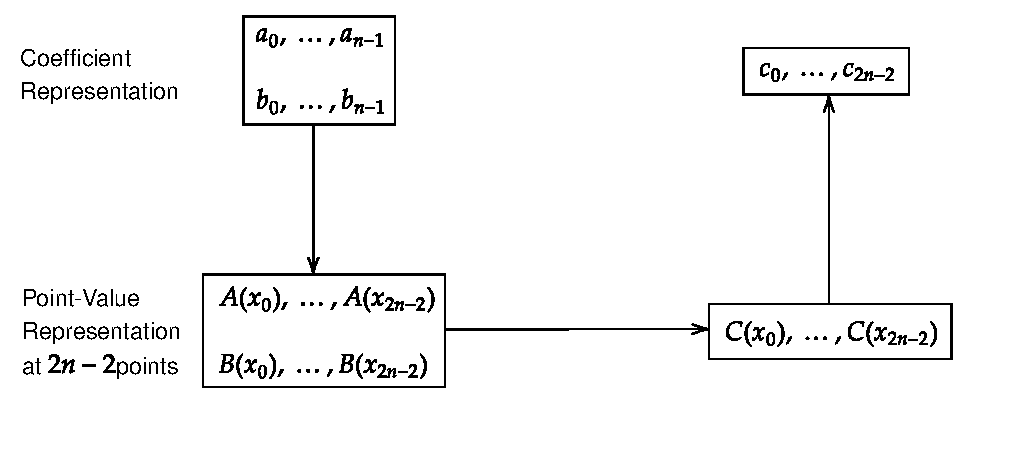
\includegraphics{images/poly-mult}
%\end{figure}
\begin{center}

\begin{tikzpicture}[node distance=3cm, thick]
	
	% Define the rectangles
	\node[draw, rectangle, minimum width=3cm, minimum height=1.5cm] (rect1) at (0, 1.5) {$ \begin{array}{l}
			a_{0} ,\dotsc ,a_{n-1}\\
			\\
			b_{0} ,\dotsc ,b_{n-1}
		\end{array}$};
	\node[draw, rectangle, minimum width=3cm, minimum height=1.5cm] at (0,-3) (rect2) {$ \begin{array}{l}
			A( x_{0}) ,\dotsc ,A( x_{2n-2})\\
			\\
			B( x_{0}) ,\dotsc ,B( x_{2n-2})
		\end{array}$};
	\node[draw, rectangle, minimum width=3cm, minimum height=1cm]  at (8, 1.5) (rect3) {$c_{0} ,\dotsc ,c_{2n-2}$};
	\node[draw, rectangle, minimum width=4cm, minimum height=1.5cm] at (8,-3) (rect4) {$C( x_{0}) ,\dotsc ,C( x_{2n-2})$};
	% Define the text blocks on the left
	\node[align=left] (text1) at (-4, 1.5) {Coefficient\\ Representation};
	\node[align=left] (text2) at (-4, -3) {Point-Value\\ Representation\\ at $\displaystyle 2n-2$ points};
	
	% Draw dotted helper lines (optional for alignment visualization)
	\draw[-Stealth] (rect1.south) -- (rect2.north);
	\draw[-Stealth] (rect2.east) -- (rect4.west);
	\draw[-Stealth] (rect4.north) -- (rect3.south);	
\end{tikzpicture}
\end{center}
\subsection{Finding Evaluations of Multiplied Polynomial}

Suppose we were given $A(x)$ and $B(x)$ evaluated at $2n-1$ distinct points $x_0,\dots, x_{2n-2}$. Then we can get $C(x)$ evaluated at $x_0,\dots, x_{2n-2}$ by $$C(x_i)=A(x_i)B(x_i)\ \forall\ i\in \llbracket 2n-2\rrbracket$$Since there are $O(n)$ many points and for each point it takes constant time to multiply we can find evaluations of $C$ at $x_0,\dots, x_{2n-2}$ in $ O(n)$ time.
\subsection{Evaluation of a Polynomial at Points}\label{fft}
\begin{question}{}{}
	Suppose there is only one point, $x_0$. Can we evaluate a $n-1$ degree polynomial $A(x)=\sum\limits_{i=0}^{n-1}a_ix^i$ at $x_0$ efficiently?
\end{question}
We can rewrite $A(x)$ as $$A(x)=a_0+x(a_1+x(a_2+x(a_3+\cdots (a_{n-1}+x(a_n))\cdots )))$$In this represent it is clear that we have to do $n$ additions and $n$ multiplications to find $A(x_0)$. Hence we can evaluate a $n-1$ degree polynomial at a point in $O(n)$ time


But we have $O(n)$ points. And if each point takes $O(n)$ time to find the evaluation of the polynomial then again it will take total $O(n^2)$ time. We are back to square one. So instead we will evaluate the polynomial in some special points and we will evaluate in all of them in $O(n\log n)$ time. So now the problem we will discuss now is to find some special $n$ points where we can evaluate a $n-1$-degree polynomial in $O(n\log n)$ time.
\parinf

\textbf{Idea:} Evaluate at roots of unity and use Fast Fourier Transform
\parinn

Assume $n$ is a power of 2. NWe have the polynomial $A(x)=\sum\limits_{i=0}^{n-1}a_ix^i$. So now consider the following two polynomials $$A^0(x)=a_0+a_2x+a_4x^2+\cdots+a_{n-2}x^{\frac{n}2-1}\qquad A^1(x)=a_1+a_3x+a_5x^2+\cdots+a_{n-1}x^{\frac{n}2-1}$$Certainly we have $$A(x)=A^0(x^2)+xA^1(x^2)$$Hence we can get $A(1)$ and $A(-1)$ by $$A(1)=A^0(1)+A^1(1)\qquad A(-1)=A^0(1)-A^1(1)$$Hence like this by evaluating two $\frac{n}2-1$ degree polynomials at one point we get evaluation of $A$ at two points. More generally for any $y\geq 0$ we have$$A(\sqrt{y})=A^0(y)+\sqrt{y}A^1(y)\qquad A(-\sqrt{y})=A^0(y)-\sqrt{y}A^1(y)$$So by recursing like this evaluating at $1,-1$ we can get evaluations of $A$ at $n^{th}$ roots of unity.

Let $$\om_n^k=n^{th}\text{ root of unity for }k\in\llbracket n-1\rrbracket = e^{i\frac{k}{n}2\pi}=\cos\lt(\frac{k}{n}2\pi\rt)+i\sin s\lt(\frac{k}{n}2\pi\rt)$$Hence we have \begin{align*}
	A\lt(\om_n^k\rt)&=A^0\lt(\om_n^{2k}\rt)+\om_n^kA^1\lt(\om_n^{2k}\rt)=A^0\lt(\om_{\frac{n}2}^{k}\rt)+\om_n^kA^1\lt(\om_{\frac{n}2}^{k}\rt)\\
	A\lt(-\om_n^k\rt)=A\lt(\om_n^{\frac{n}2+k}\rt)&=A^0\lt(\om_n^{2k}\rt)-\om_n^kA^1\lt(\om_n^{2k}\rt)=A^0\lt(\om_{\frac{n}2}^{k}\rt)-\om_n^kA^1\lt(\om_{\frac{n}2}^{k}\rt)
\end{align*}Hence now we will solve the following problem:
\begin{algoprob}
	\problemtitle{Recursive-DFT}
	\probleminput{$(a_0,\dots, a_{n-1})$ representing $(n-1)-$degree polynomial $A(x)=\sum\limits_{i=0}^{n-1}a_ix^i$}
	\problemquestion{Find the evaluations of the polynomial $A(x)$ in all $n^{th}$ roots of unity}
\end{algoprob}

\vspace*{5mm}\parinf
Since $A^0$ and $A^1$ have degree $\frac{n}2-1$ we can use recursion. Hence the algorithm is 
\begin{algorithm}\SetKwComment{Comment}{// }{}
	\DontPrintSemicolon
	\KwIn{$A=(a_0,\dots, a_{n-1})$ such that $A(x)=a_0+a_1x+\cdots+ a_{n-1}x^{n-1}$}
	\KwOut{$A(x)$ evaluated at $n^{th}$ roots of unity $\om_n^k$ for all $k\in\llbracket n-1\rrbracket$}
	\Begin{
	\If{$n==1$}{\Return{$A[0]$}}
	$A^0\longleftarrow (A[0],A[2],\dots,A[n-2])$\;	
	$A^1\longleftarrow(A[1],A[3],\dots,A[n-1])$\;
	$Y^0\longleftarrow 	\prb{Recursive-DFT}(A^0)$\;
	$Y^1\longleftarrow 	\prb{Recursive-DFT}(A^1)$\;		
	\For{$k=0$ to $\frac{n}{2}-1$}{
		
	$Y[k]\longleftarrow Y^0[k]+\om_n^kY^1[k]$\Comment*{$	A\lt(\om_n^k\rt)=A^0\lt(\om_{\frac{n}2}^{k}\rt)+\om_n^kA^1\lt(\om_{\frac{n}2}^{k}\rt)$}
	$Y\lt[k+\frac{n}{2}\rt]\longleftarrow Y^0[k]-\om_n^{\frac{n}2+k}Y^1[k]$\Comment*{$	A\lt(-\om_n^k\rt)=A^0\lt(\om_{\frac{n}2}^{k}\rt)-\om_n^kA^1\lt(\om_{\frac{n}2}^{k}\rt)$}
}
\Return{Y}
}
		\caption{\prb{Recursive-DFT}$(A)$}
	\end{algorithm}

\textbf{Time Complexity}: $T(n)=2T\lt(\frac{n}2\rt)+O(n)=O(n\log n)$.\parinn

 Therefore we can evaluate a $n-1$ degree polynomial in all the $n^{th}$ roots of unity in $O(n\log n)$ time. Hence with this algorithm we will get evaluations of the polynomial $C(x)=A(x)B(x)$ in all the $2n^{th}$ roots of unity. Now we need to interpolate the polynomial $C(x)$ from its evaluations. We will describe the process in the next subsection.
 \subsection{Interpolation from Evaluations at Roots of Unity}In this section we will show how to interpolate a $n-1$ degree polynomial from evaluations at all $n^{th}$ roots of unity. Previously we had $$\underbrace{\mat{C\lt(\om^0_n\rt)\\ C\lt(\om^1_n\rt)\\ C\lt(\om^2_n\rt)\\ \vdots\\ C\lt(\om^{n-1}_n\rt)}}_{Y}=\underbrace{\mat{1 & \om^0_n & \om ^{0\cdot 2}& \cdots & \om^{0\cdot (n-1)}\\  1 & \om^1_n & \om ^{1\cdot 2}& \cdots & \om^{1\cdot (n-1)}\\ 1 & \om^2_n & \om ^{2\cdot 2}& \cdots & \om^{2\cdot (n-1)}\\ \vdots & \vdots & \vdots & \ddots & \vdots\\ 1 & \om^{n-1}_n & \om ^{(n-1)\cdot 2}& \cdots & \om^{(n-1)\cdot (n-1)}}}_{V=\text{ Vandermonde Matrix}}\underbrace{\mat{c_0\\ c_1\\ c_2\\ \vdots \\ c_{n-1}}}_{C}$$
 
 Now vandermonde matrix is invertible since all the $n^{th}$ roots are distinct. Therefore $C=V^{-1}Y$. But we can not do a matrix inversion to interpolate the polynomial because that will take $O(n^2)$ time. Instead we have this beautiful result:
 \begin{lemma}{}{}
 	$\lt(V^{-1}\rt)_{j,k}=\frac1n\om_n^{-jk}$ for all $0\leq j,k\leq n-1$
 \end{lemma}
\begin{proof}
	Consider the matrix $n\times n$ matrix $T$ such that $(T)_{j,k}=\frac1n\om_n^{-jk}$. Now we will show $VT=I$ This will confirm that $V^{-1}=T$. Now $$\sum_{k=0}^{n-1} (V)_{i,j}\, (T)_{j,k}=\sum_{k=0}^{n-1} \om^{ij}_n\times \frac1n\om_n^{-jk}=\frac1n\sum_{k=0}^{n-1}\lt(\om^{i-k}_n\rt)^j=\begin{cases}
		\dfrac1n\dps{\sum\limits_{k=0}^{n-1}}1=1& \text{when $i=k$}\\[5mm] \dfrac1n \dfrac{1-\om^n_n}{1-\om} =0 & \text{when $i\neq k$}
	\end{cases} $$Hence in $VT$ there are $1'$s on the diagonal and rest of the locations are $0$. Hence $VT=I$. So $V^{-1}=T$.
\end{proof}
Hence we can see the inverse of the vandermonde matrix is also a vandermode matrix with a scaling factor. We will denote $y_i=C\lt(\om_n^{i}\rt)$ for $i\in\llbracket n-1\rrbracket$ since these values are given to us some how and we have to find the corresponding polynomial. Therefore we have $$\underbrace{\mat{c_0\\ c_1\\ c_2\\ \vdots \\ c_{n-1}}}_{C}=\frac1n\underbrace{\mat{1 & 1 & 1& \cdots & 1\\  1 & \om^{-1}_n & \om ^{-1\cdot 2}& \cdots & \om^{-1\cdot (n-1)}\\ 1 & \om^{-2}_n & \om ^{-2\cdot 2}& \cdots & \om^{-2\cdot (n-1)}\\ \vdots & \vdots & \vdots & \ddots & \vdots\\ 1 & \om^{-(n-1)}_n & \om ^{-(n-1)\cdot 2}& \cdots & \om^{-(n-1)\cdot (n-1)}}}_{V^{-1}}\underbrace{\mat{c_0\\ c_1\\ c_2\\ \vdots \\ c_{n-1}}}_{C}\underbrace{\mat{y_0\\ y_1\\ y_2\\ \vdots\\ y_{n-1}}}_{Y}$$
\begin{observation*}
	$nc_j=y_0+y_1\om_n^{-j}+y_2\om_n^{-2j}+\cdots+y_{n-1}\om_n^{-(n-1)j}$ for all $j\in\llbracket n-1\rrbracket$.
\end{observation*}
We can also see this situation as we have the polynomial $Y(x)=y_0+y_1x+y_2x^2+\cdots +y_{n-1}x^{n-1}$ and $c_j$ is just $Y(x)$ evaluated as $\om^{-j}_n=\om_n^{n-j}$ multiplied by $n$. Hence we just reindex the $n^{th}$ roots of unity and evaluate $Y$ $n^{th}$ roots of unity in $O(n\log n)$ time using the algorithm described in \autoref{fft}
\chapter{Dynamic Programming}
\dfnc[dynamic-prog]{Dynamic Programming}{Dynamic Programming has 3 components:\begin{enumerate}
		\item {Optimal Substructure}: Reduce problem to smaller independent problems
		\item {Recursion}: Use recursion to solve the problems by solving smaller independent problems
		\item {Table Filling}: Use a table to store the result to solved smaller independent problems.
\end{enumerate}}
\section{Longest Increasing Subsequence}
\begin{algoprob}
	\problemtitle{\prb{Longest Increasing Subsequence}}
	\probleminput{Sequence of distinct integers $A=(a_1,\dots, a_n)$}
	\problemquestion{Given an array of distinct integers find the longest increasing subsequence i.e. return maximum size set $S\subseteq[n]$ such that $\forall\ i,j\in S$, $i<j\implies a_i<a_j$}
\end{algoprob}
\subsection{\texorpdfstring{$O(n^2)$}{O(n2)} Time Algorithm}
Given $A=(a_1,\dots, a_n)$ first we will create a $n$-length array where $i^{th}$ entry stores the length and longest increasing subsequence ending at $a_i$. Certainly we have the following recursion relation$$\prb{LIS}(k)=1+\max\limits_{\substack{j<k,\  a_j<a_k}}\{\prb{LIS}(j)\}$$since if a subsequence $S\subseteq [n]$ is the longest increasing subsequence ending at $a_k$ then certainly $S-\{k\}$ is the longest increasing subsequence which ends at $a_j<a_k$ for some $j<k$. Hence, in the table we start with 1st position and using the recursion relation we fill the table from left. And after the table is filled we look for which entry of the table has maximum length. So the algorithm will be following:

\begin{algorithm}[H]
	\SetKwComment{Comment}{// }{}
	\DontPrintSemicolon
	\KwIn{Sequence of distinct integers $A=(a_1,\dots, a_n)$}
	\KwOut{Maximum size set $S\subseteq [n]$ such that $\forall\ i,j\in S$, $i<j\implies a_i<a_j$.}
	\Begin{
	Create an array $T$ of length $n$\;
	\For{$i\in[n]$}{
	$T[i][1]\longleftarrow 1+\max\{T[j][1]\colon j<k,\ a_j<a_k\}$\Comment*{Finds $\prb{LIS}[i]$}
$T[i][2]\longleftarrow T\big[T[i][1]-1\big][2]$
}	
$Index\longleftarrow \max \{T[j][1]\colon j\in[n]\}$\;
\Return{$T[Index]$}
}
\caption{\prb{LIS}$(A)$}
\end{algorithm}\parinf
\textbf{Time Complexity:} For each iteration of the loop it takes $O(n)$ time to find $\prb{LIS}[i]$. Hence, the time complexity of this algorithm is $O(n^2)$. \parinn
\subsection{\texorpdfstring{$O(n\log n)$}{O(logn)} Time Algorithm}
In the following algorithm we update the longest increasing sequence every time we see a new element of the given sequence. At any time we keep the best available sequence.
\begin{idea*}
	We can make an increasing subsequence longer by picking the smallest number for position $k$ so that there is an increasing subsequence of length $k$. Doing this we can maximize the length of the subsequence. 
\end{idea*}

\begin{Theorem}{}{}
	If $S\subseteq A$ is the longest increasing subsequence of length $t$ then for any $k\in[t]$ the number $S(k)$ is the smallest number in the subarray of $A$ starting at first  and ending at $S(k)$ such that there is an increasing subsequence of length $k$ ending at $S(k)$.
\end{Theorem}
\begin{proof}
	Assume the contrary. Suppose $\exs\ k\in[t]$ such that $k$ is the smallest number in $[t]$ such that $S(k)$ is not the smallest number to satisfy the condition. Now denote the subarray of $A$ starting at first  and ending at $S(k)$ by $A_k$. Now let $x\in A_k$ be the smallest number in $A_k$ such that there is an increasing subsequence of length $k$ ending at $x$. Certainly $x<S(k)$ by our assumption. Now since $k$ is the smallest index which does not satisfy the given condition, $\forall\ j\in[k-1]$, $S(j)$ is the smallest number in $A_j$ such that there is an increasing subsequence of length $j$ ending at $S(j)$. Then consider the subsequence $\{S(1),\dots, S(k-1),x,S(k),S(k+1),\dots, S(t)\}$. This is an increasing subsequence of $A$ and has length $t+1$. But this contradicts the minimality of $S$. Hence, contradiction \ctr Every element of $S$ follows the given condition. 
\end{proof}

So we will construct an increasing subsequence by gradually where each step this property is followed, i.e. at each step we will ensure that the sequence built at some time have the above property. So now we describe the algorithm. 
\begin{algorithm}\SetKwComment{Comment}{// }{}
	\DontPrintSemicolon
	\KwIn{Sequence of distinct integers $A=(a_1,\dots, a_n)$}	
	\KwOut{Maximum size set $S\subseteq [n]$ such that $\forall\ i,j\in S$, $i<j\implies a_i<a_j$.}
\Begin{
	Create an array $T$ of length $n$ with all entries $0$\;
	Create an array $M$ of length $n$\;
	\For{$i=1,\dots, n$}{$M[i]\longleftarrow \infty$}	
	\For{$i=1,\dots,n$}{
		$k\longleftarrow $Find the smallest index such that $M[k]\geq a_i$ using \prb{Binary-Search}\;
		$M[k]\longleftarrow a_i$\;
		$T[i]\longleftarrow M[k-1]$\Comment*{Pointer to the previous element of the sequence}
}
$l\longleftarrow $ Largest $l$ such that $M[l]$ is finite\;
Create an array $S$ of length $l$\;
\For{$i=l,\dots, 1$}{
	\If{$i=l$}{$S[l]\longleftarrow M[l]$\;
	Continue}
$S[i]\longleftarrow T\big[S[i+1]\big]$\Comment*{$T[S[i+1]]$ is pointer to previous value of sequence}
}
\Return{$(l,S)$}
}
\caption{\prb{QuickLIS}$(A)$}
\end{algorithm}\parinf

\textbf{Time Complexity:} To create the arrays and the first for loop takes $O(n)$ time. In each iteration of the for loop at line 6 it takes $O(\log n)$ time to find $k$ and rest of the operations in the loop takes constant time. So the for loop takes $O(n\log n)$ time.  Then To find $l$ and creating $S$ it takes $O(n)$ time. Then in the for loop at line 12 in each iteration it takes constant time. So the for loop at line 12 takes in total $O(n)$ time. Therefore, the algorithm takes $O(n\log n)$ time. \parinn

We will do the proof of correctness of the algorithm now.
\begin{lemma}{}{mdecreasing}
	For any index $M[k]$ is non-increasing
\end{lemma}
\begin{proof}
	Every time we change a value of $M[k]$ we replace by something smaller. So $M[k]$ is non-increasing.
\end{proof}
We denote the state of array $M$ at $i^{th}$ iteration by $M^i$. Then we have the following lemma:

\begin{lemma}{}{}
At any time $i$, $M^i[1]< M^i[2]< \cdots< M^i[n]$
\end{lemma}
\begin{proof}
We will prove this by induction on $i$. The base case follows naturally. Now for $i^{th}$ iteration suppose $M^{i-1}[k]$ is replaced by $x_i$. Then we know $\forall \ j<k$ we have $M^i[j]< x_i$. By inductive hypothesis at time $t-1$ we have $M$ as an increasing sequence. Now before replacing $M^{i-1}[k]< M^{i-1}[k+1]< \cdots M^{i-1}[n]$. Now by \lemref{th:mdecreasing} $M^{i-1}[k]$ is nonincreasing. So we still have $M^{i-1}[1]< \cdots M^{i-1}[k-1]< x_i < M^{i-1}[k+1]< \cdots < M^{i-1}[n]$. Therefore, $M^{i}$ is an increasing subsequence. Hence, but mathematical induction it holds.
\end{proof}

Now suppose at $i^{th}$ iteration $k_i$ is largest such that $M^i[k_i]<\infty$. Then $S^i$ denote the set constructed like the way we constructed at line 12--16 in the algorithm i.e. $$S^i[k_i]=M^i[k_i]\qquad \text{and}\qquad S^i[j]=T[S^i[j+1]]\quad \forall\ j\in[k_i-1]$$
\begin{lemma}{}{si-isgoodatalliterations}
	After any $i^{th}$ iteration, for $k\in[n]$ if $M^i[k]<\infty$ then $S^i[k]$ stores the smallest value in $x_1,\dots, x_i$ such that there is an increasing subsequence of size $k$ that ends in $S^i[k]$.
\end{lemma}
\begin{proof}
We will use induction on $i$. Base case: This is true after first iteration since only $M^1[1]<\infty$. So this naturally follows. 

Suppose this is true after $i$ iterations.  Now at $(i+1)^{th}$ iteration suppose $t$ be the smallest index such that $M^i[t]>x_{i+1}$. Then we have $$M^i[1]<\cdots< M^i[t-1]<x_{i+1}\leq M^i[t]<\cdots< M^i[n]\implies S^i[1]<\cdots< S^i[t-1]<x_{i+1}\leq S^i[t],\dots, S^i[k_i]$$ Now for $k\leq t-1$ it is true by the inductive hypothesis. For $k>t$ and if $M^{i+1}[k]<\infty$ then $S^{i+1}[k]$ is the smallest value in $x_1,\dots, x_{i+1}$ such that there is an increasing subsequence of size $k$ that ends in $S^{i+1}[k]$ since this was true for $i^{th}$ iteration. 

Now only the case when $k=t$ is remaining. If $S^{i+1}[k]$ does not store the smallest value in $x_1,\dots ,x_{i+1}$ to have an increasing subsequence of size $k$ ending at $S^{i+1}[k]$ then let $x_j$ was the smallest value to satisfy this condition where $j<i+1$. Then naturally $x_j<x_{i+1}$. Then $M^{i}[t]\leq x_j<x_{i+1}$. But we $t$ was the smallest number such that $M^{i}[t]\geq x_{i+1}$. Hence, contradiction. Therefore, $S^i[k]$ is the smallest value in $x_1,\dots, x_{i+1}$ to have an increasing subsequence of size $k$ ending at $S^{i+1}[k]$.  Therefore, by mathematical induction this is true for all iterations. 
\end{proof}
\begin{Theorem}{}{}
	$S$ is the longest increasing subsequence of $A$.
\end{Theorem}
\begin{proof}
	After the $n^{th}$ iteration $S^n=S$ and $k_n=l$. Hence by \lemref{th:si-isgoodatalliterations} we can say for all $k\in[l]$, $S[k]$ is the smallest number such that there is an increasing sequence of length $k$ ending at $S[k]$. Now we want to show that this increasing sequence is the longest increasing subsequence of $A$. Suppose $S$ is not the longest increasing subsequence. Let $T$ be the longest increasing subsequence of length $t>l$. Then suppose $j\leq l$ be the smallest index such that $S[j]\neq T[j]$. Now $S[j]$ is the smallest number in $x_1,\dots, x_n$ such that there is an increasing subsequence of length $j$ ending at $S[j]$. Hence, we have $S[j]<T[j]$. Now for all $i<j$ we have $S[i]=T[i]$.   Then we form this new subsequence $\hat{T}=\{T[1],T[2],\dots, T[j-1], S[j],T[j],\dots, T[t]\}$. Certainly $\hat{T}$ has length $t+1$ and it is also an increasing subsequence. But this contradicts the maximal condition of $T$. Hence, $S$ is indeed the longest increasing subsequence.
\end{proof}

\section{Optimal Binary Search Tree}
\begin{algoprob}
	\problemtitle{Optimal BST}
	\probleminput{A sorted array $A=(a_1,\dots, a_n)$ of search keys and an array of their probability distributions $P=(p(a_1),\dots, p(a_n))$}
	\problemquestion{Given array of keys $A$ and their probabilities the probability of accessing $a_i$ is $p(a_i)$ then return a binary tree  with the minimum cost where for any binary tree $T$, $\prb{Cost}(T)=\sum\limits_{i=1}^np(a_i)\cdot height\st_T(a_i)$.}
\end{algoprob}

So let $T$ be the optimal binary search tree with $a_k$ as its root for some $k\in[n]$. Let $T_l$ and $T_r$ denote the tree rooted at the left child and right child of $a_k$ in $T$ respectively. Then: \begin{align*}
	\prb{Cost}(T) & = p_k+ {\sum_{i<k}p_i\lt(1+height\st_{T_l}(a_i)\rt)}+{\sum_{i>k}p_i\lt(1+height\st_{T_r}(a_i)\rt)} = \sum_{i=1}^n p_i+\underbrace{\sum_{i<k}p_i \cdot height\st_{T_l}(a_i)}_{\prb{Cost}(T_l)}+\underbrace{\sum_{i>k}p_i \cdot height\st_{T_l}(a_i)}_{\prb{Cost}(T_r)}
\end{align*}
In general we will use the notation $\prb{OPTCost}(i,k)=\prb{Cost}(T_i^k)$ where $T_i^k$ is the optimal binary tree of the subarray $A[i\dots k]$ for any $i\leq k\leq n$.  Therefore, we arrive at the following recurrence relation $$\prb{OPTCost}(i,k)=\begin{cases}
	0&\text{when $i>k$}\\
	\sum\limits_{j=i}^k p(a_j)+\min\limits_{i\leq r\leq k}\{\prb{OPTCost}(i,r-1)+\prb{OPTCost}(r+1,k)\} & \text{otherwise}
\end{cases}$$
So the algorithm for constructing the optimal binary search tree is following:
\begin{algorithm}
\SetKwComment{Comment}{// }{}
\DontPrintSemicolon
\caption{\prb{OptimalBST}$(A,P)$}
\KwIn{A sorted array $A=(a_1,\dots, a_n)$ of search keys and an array of their probability distributions $P=(p(a_1),\dots, p(a_n))$}
\KwOut{Binary Tree $T$ with the minimum search cost, $\prb{Cost}(T)=\sum\limits_{i=1}^np(a_i)\cdot height\st_T(a_i)$}
\Begin{
	\For{$i=1,\dots, n$}{$\prb{OPTCost}[i,i]\longleftarrow (p(a_i),a_i)$, 
	$\prb{OPTCost}[0,i]\longleftarrow (0,None)$
}	
	\For{$d=2,\dots, n$}{
		\For{$i\in[n+1-d]$}{
			$minval\longleftarrow 0$ \;
			\For{$k=i+1,\dots, i+d-2$}{
				$newval\longleftarrow \prb{OPTCost}[i,k-1][1]+\prb{OPTCost}[k+1,i+d-1][1]$\;
				\If{$minval>newval$}{$minval\longleftarrow newval$\;
				$Index\longleftarrow k$}
			}
			$\prb{OPTCost}[i,i+d-1]\longleftarrow \lt(minval+\sum\limits_{k=1}^{i+d-1}p(a_k), k\rt)$\;
			$a_k.left\longleftarrow \prb{OPTCost}[i,k-1][2]$\;
			$a_k.right\longleftarrow \prb{OPTCost}[k+1,i+d-1][2]$
					
	}
}
\Return{\prb{OPTCost}$[1,n]$}
}
\end{algorithm}\parinf

\textbf{Time Complexity:} To two for loops at line 4 and line 5 takes $O(n^2)$ many iterations. Now the innermost for loop at line 7 runs $O(n)$ iterations where in each iteration it takes constant runtime. So the total running time of the algorithm is $O(n^3)$.
\chapter{Greedy Algorithm}

\section{Maximal Matching}

\begin{algoprob}
	\problemtitle{Maximal Matching}
	\probleminput{Graph $G=(V,E)$}
	\problemquestion{Find a maximal matching $M\subseteq E$ of $G$}
\end{algoprob}
Before diving into the algorithm to find a matching or maximal matching we first define what is a matching.
\begin{Definition}{Matching}{}
	For a graph $G=(V,E)$ a matching $M\subseteq E$ is a set of edges such that no two edges in $M$ are incident on same vertex.
\end{Definition}
\begin{Definition}{Maximal Matching}{}
	For a graph $G=(V,E)$ a matching $M\subseteq E$ is maximal if it cannot be extended and still by adding an edge.
\end{Definition}
There is also a maximum matching which can be easily understood from the name:
\begin{Definition}{Maximum Matching}{}
	For a graph $G=(V,E)$ a matching $M\subseteq E$ is maximum if it is maximal and has the maximum size among all the maximal matchings.
\end{Definition}

\begin{idea*}
	The idea is to create a maximal matching we will just go over each edge one by one and check if after adding them to the set $M$  the matching property still holds. 
\end{idea*}
\begin{algorithm}
	\SetKwComment{Comment}{// }{}
	\DontPrintSemicolon
	\KwIn{Graph $G=(V,E)$}
	\KwOut{Maximal Matching $M\subseteq E$ of $G$}
	\Begin{
	$M\longleftarrow \emptyset$\;
	Order the edges $E=\{e_1,\dots, e_k\}$ arbitrarily\;
	\For{$e\in E$}{\If{$M\cup \{u\}$ is matching}{$M\longleftarrow M\cup \{e\}$}}
	\Return{$M$}	
}
\caption{\prb{Maximal-Matching}}
\end{algorithm}

\begin{question}{}{}
		Do we always get the largest possible matching?
\end{question}
\solve{ Clearly algorithm output is not optimal always. We get a maximal matching sure. But we don't get a maximum matching always. For example the following graph
	\begin{center}
		\begin{tikzpicture}
			\draw (-2,0) circle (2pt) node (A){};
			\draw (0,0) circle (2pt) node (B){};
			\draw (2,0) circle (2pt) node (C){};
			\draw (4,0) circle (2pt) node (D){};
			\draw[blue, thick] (A) -- node[midway, above]{$e_1$} (B);
			\draw[red, thick] (B) -- node[midway, above]{$e_3$}(C);
			\draw[blue, thick] (C) -- node[midway, above]{$e_2$} (D);
		\end{tikzpicture}
	\end{center}
	If we start from $e_1$ we get the matching $\{e_1.e_2\}$ which is maximum matching but if we start from $e_3$ then we get only the maximal matching $\{e_3\}$ which is not maximum.}

 Since the algorithm output may not be optimal always we can ask the following question
 \begin{question}{}{}
 	How large is the matching obtained compared to the maximum matching?
 \end{question}
This brings us to the following result:

\begin{Theorem}{}{}
	For any graph $G$ let the greedy algorithm obtains the matching $M$ and the maximum matching is $M^{\star}$. Then $$|M|\geq \frac12|M^\star|$$
\end{Theorem}
\begin{proof}
	Consider an edge $e\in M^{\star}$ but $e\notin M$. Since $e$ wasn't  picked in $M$, $\exs\ e'\in M\setminus M^{\star}$ such that $e$ and $e'$ are incident on same vertex. Thus define the function $f:M^{\star}\to M$ where $$f(e)=\begin{cases}
		e&\text{when $e\in M$}\\
		e' & \text{when $e\in M^{\star}\setminus M$ where $e'\in M\setminus M^{\star}$ such that $e'\cap e\neq \emptyset$}
	\end{cases}$$

Now note that there are at most  two edges in $M^{\star}$ that are adjacent to an edge $e'\in M$ which will be mapped to $e'$. Hence $$|M\setminus M^{\star}|\geq \frac12 |M^{\star}\setminus M|$$Therefore $|f^{-1}(e')|\leq 2$ $\forall\ e'\in M$. Hence $$|M^\star|=|M\cap M^{\star}|+|M^{\star}\setminus M|\leq |M\cap M^{\star}||+2|M\setminus M^{\star}|\leq 2|M|$$Therefore we have the result $|M|\geq \frac12|M^{\star}|$. 
\end{proof}
\begin{alternate-proof} 
	Let $M_1$ and $M_2$ are two matchings. Consider the symmetric difference $M_1\triangle M_2$.  This consists of edges that are in exactly one of $M_1$ and $M_2$. Now in $M\triangle M^{\star}$ we have the following properties:
	\begin{enumerate}[label=(\alph*)]
		\item Every vertex in $M\triangle M^{\star}$ has degree $\leq 2\implies $ Each component is a path or an even cycle. 
		\item The edges of $M$ and $M^{\star}$ alternate. 
			\end{enumerate}
		Now we will prove the following property about the connected components of $M\triangle M^{\star}$.
		
\begin{center}
					
	\begin{minipage}{0.9\textwidth}
			\textit{\textbf{Claim:}}\hspace{1em} No connected component is a single edge. 
		
		\begin{proof}
			This is because let $e$ be a connected component. So the two edges $e_1,e_2$ which are adjacent to $e$,  they are either in both $M$ and $M^{\star}$ or not in $M$ and $M^{\star}$. The former case is not possible because then $e_1,e_2,e$ are all in either $M$ or $M^{\star}$ which is not possible as they do not satisfy the condition of matching. For the later case since $M^{\star}$ is maximal matching, $e\in M^{\star}$. Then $e\notin M$. That means $e,e_1,e_2\notin M$ which is not possible since $M$ is also a maximal matching. Therefore no connected component is a single edge.
		\end{proof}
	\end{minipage}
\end{center}

	
		Therefore every path has length $\geq 2$. Therefore ratio of $\#$ edges of $M$ to $\#$ edges of $M^{\star}$ in a path is $\leq 2$. And for cycles we have $\#$ edges of $M=\#$ edges of $M^{\star}$. So in every connected component $C$ of $M\triangle M^{\star}$ the ratio $\frac{|M^{\star}\cap C|}{|M\cap C|}\leq 2$. Therefore we have $$\frac{|M^{\star}|}{|M|}=\frac{|M\cap M^{\star}|+\sum\limits_{C}|M^{\star}\cap C|}{|M\cap M^{\star}|+\sum\limits_{C}|M\cap C|}\leq 2$$Hence we have $|M|\geq \frac12|M^\star|$.
		

\end{alternate-proof}
\section{Huffman Encoding}
\begin{algoprob}
	\problemtitle{Huffman Coding}
	\probleminput{$n$ symbols $A=(a-1,\dots, a_n)$ and their frequencies $P=(f_1,\dots, f_n)$ of using symbols}
	\problemquestion{Create a binary encoding such that: \begin{itemize}[itemsep=-0.2cm]
			\item Prefix Free: The code for one word can not be prefix for another code
			\item Minimality: Minimize $\prb{Cost}(b)=\sum\limits_{i=1}^n f_i\cdot \prb{Len}(b(a_i))$ where $b:A\to \{0,1\}^*$ is the binary encoding
	\end{itemize}}
\end{algoprob}

Assignment of binary strings can also be scene as placing the symbols in a binary tree where at any node $0$ means left child and $1$ means right child. Then the first condition implies that there can not be two codes which lies in the same path from the root to a leaf. I.e. it means that all the codes have to be in the leaves. Then the length of the binary coding for a symbol  is the height of the symbol in the binary tree. 

We can think the frequencies as the probability of appearing for a letter. We denote the probability of appearing of the letter $a_i$ by $p(a_i)\coloneqq \frac{f_i}{\sum\limits_{i=1}^nf_i}$. So the we can see the updated cost function $$\prb{Cost}(b)=\sum\limits_{i=1}^n p(a_i)\cdot\prb{Len}(b(a_i))$$And from now on we will see the frequencies as probabilities and cost function like this

\subsection{Optimal Binary Encoding Tree Properties}
Then our goal is to finding a binary tree with minimum cost where all the symbols are at the leaves. We have the following which establish the optimality of Huffman encoding over all prefix encodings where each symbol is assigned a unique string of bits.
\begin{lemma}{}{least-frequent-max-height}
	In the optimal encoding tree  least frequent element has maximum height.
\end{lemma}
\begin{proof}
	Suppose that is not the case. Let $T$ be the optimal encoding tree and let the least frequent element $x$ is at height $h_1$ and the element with the maximum height is $y$ with height $h_2$ and we have $h_1<h_2$.  Then we construct a new encoding tree $T'$ where we swap the positions of $x$ and $y$. So in $T'$ height of $y$ is $h_1$ and height of $x$ is $h_2$. Then $$\prb{Cost}(T)-\prb{Cost}(T')=(p(x)h_1+p(y)h_2)-(p(x)h_2+p(y)h_1)=(p(x)-p(y))(h_1-h_2)$$Since $p(x)<p(y)$ and $h_1<h_2$ we have $\prb{Cost}(T)-\prb{Cost}(T')>0$. But that is not possible since $T$ is the optimal encoding tree. So $T$ should have the minimum cost. Hence contradiction. $x$ has the maximum height.
\end{proof}

\begin{lemma}{}{complete-tree}
	The optimal encoding binary tree must be complete binary tree. (i.e. every non-leaf node has exactly $2$ children)
\end{lemma}
\begin{proof}
	Suppose $T$ be the optimal binary tree and there is a non-leaf node $r$ which has only one child at height $h$. 
	By \lmref{least-frequent-max-height} the least frequent element $x$ has the maximum height, $h_m$. 
	
	 Then consider the new tree $\hat{T}$ where we place the least frequent element at height $h$ and make it the second child of the node $r$. Then $$\prb{Cost}(T)-\prb{Cost}(\hat{T})=p(x)h_m-p(x)h=p(x)(h_m-h)>0$$But this is not possible as $T$ is the optimal binary tree and it has the minimal cost. Hence contradiction. Therefore the optimal encoding binary tree must be a complete binary tree. 
\end{proof}
\begin{lemma}{}{least-frequents-siblings}
There is an optimal binary encoding tree such that the least frequent element and the second least frequent element are siblings at the maximum height.
\end{lemma}
\begin{proof}
Let $T$ be optimal binary encoding tree. Suppose $x$, $y$ are the least frequent element and the second least frequent element. And suppose $b$, $c$  be two siblings at the maximum height of the tree (There may be many such siblings, and if so pick any such pair.). If $\{x,y\}=\{b,c\}$ we are done. So suppose not. Let the frequencies of $x,y,b,c$ are respectively $p(x),p(y),p(b),p(c)$ and heights of $x,y,b$ are $h_x,h_y$ and $h$ respectively.  WLOG assume $p(x)\leq p(y)$ and $p(b)\leq p(c)$. 

Now since we know $x,y$ have the smallest frequencies we have $p(x)\leq p(b)$ and $p(y)\leq p(c)$. And since $b,c$ have the maximum height we have $h_x,hy\geq h$. So we switch the position of $x$ with $b$ to form the new tree $T'$. And from $T'$ we swap the positions fo $y$ and $c$ to form a new tree $T''$.

\begin{center}
	\begin{tikzpicture}[
		every node/.style={font=\sffamily, align=center, line width=0.15mm},
		level 1/.style={level distance=1cm, sibling distance=2cm},  % Adjusted distance for level 1
		level 2/.style={sibling distance=2cm},   % Adjusted distance for level 2
		square/.style={draw, shape=rectangle, minimum width=0.5cm, minimum height=0.5cm, inner sep=0pt, text width=0.5cm, text centered},
		circle/.style={draw, shape=circle, minimum width=0.5cm, minimum height=0.5cm, inner sep=0pt, text width=0.5cm, text centered},
		filled/.style={fill=blue!20, , draw, line width=0.12mm},  % Style for filled nodes
		every edge/.style = {draw, latex'-latex' , line width=0.3mm, dotted,},
		parentarrow/.style={line width=0.12mm, -{latex[length=1mm, width=0.2mm, open, round]}},  % Style for arrows from nodes to children
		]
		
		% Leftmost tree
		\node[circle] (A1) {}
		child {node[circle] (B1) {}
			child {node[square] (D1) {$y$} edge from parent[parentarrow]}
			child {node[circle] (E1) {}
				child {node[square] (F1) {$c$} edge from parent[parentarrow]}
				child {node[square, filled] (G1) {$b$} edge from parent[parentarrow]}
				edge from parent[parentarrow]
			}
		edge from parent[parentarrow]
		}
		child {node[square,filled] (C1) {$x$} edge from parent[parentarrow]};
		\node[above left=0cm and 0cm of A1] (T1) {$T$};  % Label T1
		% Middle tree
		\node[circle, right=4cm of A1] (A2) {}
		child {node[circle] (B2) {}
			child {node[square, filled] (D2) {$y$} edge from parent[parentarrow]}
			child {node[circle] (E2) {}
				child {node[square, filled] (F2) {$c$} edge from parent[parentarrow]}
				child {node[square] (G2) {$x$} edge from parent[parentarrow]}
				edge from parent[parentarrow]
			}
			edge from parent[parentarrow]
		}
		child {node[square] (C2) {$b$} edge from parent[parentarrow]};
		\node[above left=0cm and 0cm of A2] (T1) {$T'$};  % Label T2
		
		% Rightmost tree
		\node[circle, right=4cm of A2] (A3) {}
		child {node[circle] (B3) {}
			child {node[square] (D3) {$c$}edge from parent[parentarrow]}
			child {node[circle] (E3) {}
				child {node[square] (F3) {$y$} edge from parent[parentarrow]}
				child {node[square] (G3) {$x$} edge from parent[parentarrow]}
				edge from parent[parentarrow]
			}
		edge from parent[parentarrow]
		}
		child {node[square] (C3) {$b$} edge from parent[parentarrow]};
		\node[above left=0cm and 0cm of A3] (T1) {$T''$};  % Label T3
		
		
		% Dotted bidirectional bent arrows between leaf nodes D and E in each tree
		\draw (C1) edge[bend left=45] (G1);
		\draw (F2) edge[bend left=45] (D2);
		
		% Arrows from leftmost tree to middle tree and from middle tree to rightmost tree
		\draw[-Latex, thick, shorten <= 1mm, shorten >= 1mm] (A1) -- (A2);
		\draw[-Latex, thick, shorten <= 1mm, shorten >= 1mm] (A2) -- (A3);
		
	\end{tikzpicture}
\captionof{figure}{Showing that the lowest probability nodes are siblings at the tree’s lowest level.} 
\label{fig:least-frequent-elm-siblings}
\end{center}

Now we will calculate how the cost changes as we go from $T$ to $T'$ and $T'$ to $T''$. First check for $T\to T'$. Almost all the nodes contribute the same except $x,b$. So we have $$\prb{Cost}(T)-\prb{Cost}(T')=(h_x\cdot p(x)+h\cdot p(b))-(h_x\cdot p(b)+h\cdot p(x))=(p(b)-p(x))(h-h_x)\geq 0$$Therefore swapping $x$ and $b$ does not increase the cost and since $T$ is the optimal binary encoding tree the cost doesn't decrease either. Therefore the costs are equal. Hence $T'$ is also an optimal tree. 

Similarly we calculate cost for going from $T'$ to $T''$ we have $$\prb{Cost}(T')-\prb{Cost}(T'')=(h_y\cdot p(y)+h\cdot p(c))-(h_y\cdot p(c)+h\cdot p(y))=(p(c)-p(y))(h-h_y)\geq 0$$Therefore swapping $y$ and $c$ also does not increase the cost and since $T'$ is the optimal binary encoding tree the cost doesn't decrease either. Therefore the costs are equal. Hence $T''$ is also an optimal tree. Hence $T''$ is the optimal tree where the least frequent element and second last frequent element are siblings.
\end{proof}




By the \lmref{complete-tree} and \lmref{least-frequents-siblings} we have that the least frequent element and the second least frequent element are siblings and they have the maximum height.

%\begin{Theorem}{}{replace-less-variable-case}
%Let $T_n$ be any optimal binary encoding tree following \lmref{least-frequents-siblings} (i.e. lowest probability symbols $x$ and $y$ are siblings at the deepest level). Let $T_{n-1}$ be the tree that results by replacing these two leaf nodes for $x,y$  and their parent with a single leaf node $z$ of probability $p(z)=p(x)+p(y)$. Then $$\prb{{Cost}}(T_n)=\prb{Cost}(T_{n-1})+p(z)$$
%\end{Theorem}
%\begin{proof}
%	Let $h$ be the heights of $x$ and $y$ in $T_n$. Clearly $z$ is in height $h-1$ in $T_{n-1}$. Since $z$ replaces $x$ and $y$ the costs of the two trees satisfies \begin{align*}
%		\prb{Cost}(T_n)&=\prb{Cost}(T_{n-1})-(\text{\prb{Cost} due to $z$ in \prb{Cost}$(T_{n-1})$} + (\text{\prb{Cost} due to $x$ and $y$ in \prb{Cost}$(T_{n})$})\\
%		& =\prb{Cost}(T_{n-1})-p(z)\cdot (d-1)+(p(x)+p(y))\cdot d\\
%		& = \prb{Cost}(T_{n-1})-p(z)\cdot (d-1)+p(z)\cdot d\\
%		& = \prb{Cost}(T_{n-1})+p(z)
%	\end{align*}
%\end{proof}

\begin{observation*}
	The cost of the trees $T_n$ and $T_{n-1}$ differ only by the fixed term $p(z)=p(x)+p(y)$ which does not depend on the tree's structure. Therefore minimizing the cost for $T_n$ is equivalent to minimizing the cost of $T_{n-1}$.
\end{observation*}
\begin{Theorem}{}{replace-less-variable-case}
	Given an instance with symbols $\mcI$: \begin{center}
		\begin{tabular}{ccccccccc}
			$a_1$, & $a_2$, & $\cdots$, & $a_i$, & $\cdots$, & $a_j$, & $\cdots$, & $a_n$ & with probabilities\\
			$p(a_1)$, & $p(a_2)$, & $\cdots$, & $p(a_i)$, & $\cdots$, & $p(a_j)$, & $\cdots$, & $p(a_n)$ &
		\end{tabular} 
	\end{center}
	such that $a_i$, $a_j$ are the least frequent and second least frequent elements respectively. Consider the instance with $n-1$ symbols $\mcI'$:
	\begin{center}
		\begin{tabular}{ccccccccccc}
			$a_1$, & $a_2$, & $\cdots$, & $a_{i-1}$, & $a_{i+1}$,& $\cdots$, & $a_{j-1}$,& $a_{j+1}$, & $\cdots$, & $a_n$, & $z$ \\
			$p(a_1)$, & $p(a_2)$, & $\cdots$, & $p(a_{i-1})$,&$p(a_{i+1})$  & $\cdots$, & $p(a_{j-1})$,& $p(a_{j+1})$, & $\cdots$, & $p(a_n)$, & $p(a_i)+p(a_j)$ 
		\end{tabular} 
	\end{center}
	Let $T'$ be the optimal tree for this instance $\mcI'$. Then there is an optimal tree for the original instance $\mcI$ obtained from $T'$ by replacing the leaf of $b$ by an internal node with children $a_i$ and $a_j$.
\end{Theorem}
\begin{proof}
	We will prove this by contradiction. Suppose $\hat{T}$ is optimal for $\mcI$. Then $\prb{Cost}(\hat{T})<\prb{Cost}(T)$. In $\hat{T}$ we know $a_i$ and $a_j$ are siblings by \lmref{least-frequents-siblings}. Now consider $\hat{T}'$ for instance $\mcI'$ where we merge $a_i,a_j$ leaves and their parent into a leaf for symbol $z$. 
	
	\begin{center}
		\usetikzlibrary{fit}
		\begin{tikzpicture}[
			every node/.style={font=\sffamily, align=center, line width=0.15mm},
			level 1/.style={level distance=1cm, sibling distance=2cm},  % Adjusted distance for level 1
			level 2/.style={sibling distance=2cm},   % Adjusted distance for level 2
			square/.style={draw, shape=rectangle, minimum width=0.5cm, minimum height=0.5cm, inner sep=0pt, text width=0.5cm, text centered},
			circle/.style={draw, shape=circle, minimum width=0.5cm, minimum height=0.5cm, inner sep=0pt, text width=0.5cm, text centered},
			filled/.style={fill=blue!20, , draw, line width=0.12mm},  % Style for filled nodes
			every edge/.style = {draw, latex'-latex' , line width=0.3mm, dotted,},
			parentarrow/.style={line width=0.12mm, -{latex[length=1mm, width=0.2mm, open, round]}},  % Style for arrows from nodes to children
			dottedoval/.style={draw, line width=0.3mm, densely dotted, inner sep=0.2mm, ellipse, minimum width=1cm, minimum height=1.5cm}, % Style for the dotted oval shape
			]
			
			% Leftmost tree
			\node[circle] (A1) {}
			child {node[circle] (B1) {}
				child {node[circle] (D1) {} edge from parent[parentarrow]}
				child {node[circle, filled] (E1) {}
					child {node[square, filled] (F1) {$a_i$} edge from parent[parentarrow]}
					child {node[square,filled] (G1) {$a_j$} edge from parent[parentarrow]}
					edge from parent[parentarrow]
				}
				edge from parent[parentarrow]
			}
			child {node[circle] (C1) {} edge from parent[parentarrow]};
			\node[above left=0cm and 0cm of A1] (T1) {${T}$};  % Label T1
			% Middle tree
			\node[circle, left=4cm of A1] (A2) {}
			child {node[circle] (B2) {}
				child {node[circle] (D2) {} edge from parent[parentarrow]}
				child {node[square, filled] (E2) {$z$}}
				edge from parent[parentarrow]
			}
			child {node[circle] (C2) {} edge from parent[parentarrow]};
			\node[above left=0cm and 0cm of A2] (T1) {${T}'$};  % Label T2
			\draw[-Latex, thick, shorten <= 1mm, shorten >= 1mm] (A2) -- (A1);
			% Dotted oval shape containing E1, F1, and G1
			\node[dottedoval, fit=(E1)(F1)(G1), yshift=-0.15cm] (Oval) {};
			
			% Arrow from dotted oval to B1
			\draw[-latex, dottedoval] (E2) to[out=-90,in=-150] (Oval);
		\end{tikzpicture}
	\end{center}
	
	Then $$\prb{Cost}(\hat{T}')=\prb{Cost}(\hat{T})-p(a_i)-p(a_j)<\prb{Cost}(T)-p(a_i)-p(a_j)=\prb{Cost}(T')$$This contradicts the fact that $T'$ is optimal binary encoding tree for $\mcI'$. Hence $T$ is optimal.
\end{proof}




\subsection{Algorithm}
\begin{idea}
	We are going to build the tree up from the leaf level. We will take two characters $x,y$, and ``merge” them into a single character, $z$, which then replaces $x$ and $y$ in the alphabet. The character $z$ will have  probability
	equal to the sum of $x$ and $y$’s probabilities. Then we continue recursively building the code on
	the new alphabet, which has one fewer character.
\end{idea}

Since we always need the least frequent element and the second least frequent element we have to use the data structure called \prb{Min-Priority Queue}. So the following algorithm uses a \prb{Min-Priority Queue} $Q$ keyed on the probabilities to identify the two least frequent objects. 

%\newpage 
\begin{algorithm}
	\SetKwComment{Comment}{// }{}
	\DontPrintSemicolon
	\KwIn{Set of $n$ symbols $A=\{a_1,\dots, a_n\}$ and their probabilities $P=\{p_1,\dots, p_n\}$}
	\KwOut{Optimal Binary Encoding $b:A\to \{0,1\}^*$ for $A$ with minimum $\prb{Cost}(b)=\sum\limits_{i=1}^n p(a_i)\cdot\prb{Len}(b(a_i))$.}
	\Begin{
	$n\longleftarrow |A|$\;
	$Q\longleftarrow$ \prb{Min-Priority Queue}\;
	\For{$x\in A$}{\prb{Insert}$(Q,x)$}
	\For{$i=1,\dots n-1$}{$z\longleftarrow $ New internal tree node\;
		$x\longleftarrow $ \prb{Extract-Min}$(Q)$,		$y\longleftarrow $ \prb{Extract-Min}$(Q)$\;
	$left[z]\longleftarrow x$, 
$right[z]\longleftarrow y$\;
$p(z)\longleftarrow p(x)+p(y)$\;
$\prb{Insert}(Q,z)$
}
\Return{Last element left in $Q$ as root}
}
\caption{\prb{Huffman-Encoding}$(A,P)$}
\end{algorithm}

\parinf
\textbf{Time Complexity:} To create the priority queue it takes $O(n)$ time in line 4-5. Then for each iteration of the for loop in line 6 the \prb{Extract-Min} operation takes $O(\log n)$ time and then to insert an element it also takes $O(\log n)$ time. Hence each iteration takes $O(\log n)$ time. Since the for loop has $n-1=O(n)$ many iterations the running time for the algorithm is $O(n\log n)$. 

\begin{remark}
	We can reduce the running time to $O(n\log\log n)$ by replacing the binary min-heap with a van Emde Boas tree.
\end{remark}

\begin{Theorem}{Correctness of Huffman's Algorithm}{}
	The above Huffman's algorithm produces an optimal prefix code tree
\end{Theorem}
\begin{proof}
	We will prove this by induction on $n$, the number of symbols. For base case $n=1$. There is only one tree possible.
	
	For $n=k$ we know that by \lmref{least-frequents-siblings} and \lmref{least-frequent-max-height} that the two symbols $x$ and $y$ of lowest probabilities are siblings and they have the maximum height. Huffman's algorithm replaces these nodes by a character $z$ whose probability is the sum of their probabilities. Now we have 1 less symbols. So by inductive hypothesis Huffman's algorithm computes the optimal binary encoding tree for the $k-1$ symbols. Call it $T_{n-1}$. Then the algorithm replaces $z$ with a parent node with children $x$ and $y$ which results in a tree $T_n$ whose cost is higher by a fixed amount $p(z)=p(x)+p(y)$. Now since $T_{n-1}$ is optimal by \thmref{replace-less-variable-case} we have $T_n$ is also optimal.
\end{proof}
\section{Matroids}
\dfn{Matroid}{A matroid $M=(E,\mcI)$ has a ground set $E$ and a collection $I$ of subsets of $E$ called the \textit{Independent Sets} st\begin{enumerate}
		\item Downward Closure: If $Y\in \mcI$ then $\forall \ X\subseteq Y$, $X\in \mcI$.
		\item Exchange Property: If $X,Y\in \mcI$, $|X|<|Y|$ then $\exs\ e\in Y-X$ such that $X\cup \{e\}$ also written as $X+e\in \mcI$
\end{enumerate}}
An element $x\in E$ extends $A\in\mcI$ if $A\cup \{x\}\in\mcI$. And $A$ is maximal if no element can extend $A$.
\begin{lemma}{}{}
	If $A,B$ are maximal independent set, then $|A|=|B|$ i.e. all maximal independent sets are also maximum
\end{lemma}
\begin{proof}
	Suppose $|A|\neq |B|$. WLOG assume $|A|>|B|$. Then by the exchange property $\exs\ e\in A-B$ such that $B\cup \{e\}\in\mcI$. But we assumed that $B$ is maximal independent set. Hence contradiction. We have $|A|=|B|$.
\end{proof}
\parinf

\textbf{Base:} Maximal Independent sets are called bases.

\textbf{Rank of $\boldsymbol{S\in I}$:} $\max\{|X|\colon X\subseteq S, X\in I\}$

\textbf{Rank of a Matroid:} Size of the base.

\textbf{Span of $\boldsymbol{S\in I}$:} $\{e\in E\colon rank(S)=rank(S+e)\}$



\subsection{Examples of Matroid}
\begin{itemize}[label=$\bullet$]
\item \textbf{Uniform Matroid:} Given $E=\{e_1,\dots, e_n\}$, and $k\in\bbZ_0$ take $\mcI=\{S\subseteq E\colon |S|\leq k\}$
\begin{lemma}{}{}
	$M=(E,\mcI)$ defined as above is a matroid
\end{lemma}
\begin{proof}
	\begin{enumerate}[label=\bfseries\tiny\protect\circled{\small\arabic*}]
		\item Downward Closure: $A\in \mcI$, $B\subseteq A\implies |B|\leq k\implies B\in \mcI$
		\item Exchange Property: $A,B\in\mcI,\ |B|<|A|\leq k\implies |B|<k\implies \forall\ e\in A-B,\ |B\cup \{e\}|\leq k\implies B\cup \{e\}\in \mcI$
	\end{enumerate}
Therefore $M$ is a matroid
\end{proof}
\item \textbf{Partition Matroid:} Given $E$, $\{P_1,\dots, P_l\}$ such that $E=\bigsqcap\limits_{i=1}^lP_i$ and $k_1,\dots, k_l\in\bbZ_0$ then take $$\mcI=\{S\subseteq E\colon \forall\ k\in[l],\ |S\cap P_j|\leq k_j\}$$
\begin{lemma}{}{}
	$M=(E,\mcI)$ defined as above is a matroid
\end{lemma}
\begin{proof}
		\begin{enumerate}[label=\bfseries\tiny\protect\circled{\small\arabic*}]
		\item Downward Closure: $A\in \mcI$, $B\subseteq A\implies \forall\ j\in[l]\ |B\cap P_j|\leq |A\cap P_j|\leq k_j\implies B\in \mcI$
		\item Exchange Property: $A,B\in\mcI,\ |B|<|A|\implies \exs \ j\in[l],\ |B\cap P_j|< |A\cap P_j|\leq k_j\implies e\in (A\cap P_j)-{(B\cap P_j)}, \ |(B\cup\{e\})\cap P_j|=|B\cap P_j|+1\leq k\implies B\cup \{e\}\in\mcI$
	\end{enumerate}Therefore $M$ is a matroid
\end{proof}
\item \textbf{Laminar Matroid:} Given $E$, $\sL=\{L_1,\dots,L_l\}$ such that $\forall\ i,j\in [l]$, either $L_i\subseteq L_j$ or $L_i\supseteq L_j$ or $L_i\cap L_j=\emptyset$ and also given $k_1,\dots, k_l\in \bbZ_0$. Then take $$\mcI=\{S\subseteq E\colon \forall \ j\in[l],\ |S\cap L_j|\leq k_j\}$$For any $L\in\sL$ we denote $k(L)$ be the given number corresponding to $L$.
\begin{lemma}{}{laminar-matroid}
	$M=(E,\mcI)$ defined as above is a matroid
\end{lemma}
\begin{proof}
	\begin{enumerate}[label=\bfseries\tiny\protect\circled{\small\arabic*}]
		\item Downward Closure: $A\in \mcI$, $B\subseteq A\implies \forall\ j\in[l]\ |B\cap L_j|\leq |A\cap L_j|\leq k_j\implies B\in \mcI$
		\item Exchange Property: \parinn Let $A,B\in \mathcal{I}$ with $|B|<|A|$.	If there exists $e\in A\backslash B$ such that $e\notin L$ for any $L\in\sL$, then $|(B+e)\cap L|=|B\cap L|\leq k(L)$ for any $L\in\sL$.
		
		Hence assume that for each $e\in A\backslash B$ there exists $L\in\sL$ with $e\in L$.
		For each $e\in A\backslash B$, let $\sL_e$ be the collection of $L\in\sL$ with $e\in L$.
		For each $e\in A\backslash B$ and any $L\in\sL\backslash\sL_e$, we have $|(B+e)\cap L|=|B\cap L|\leq k(L)$.
		
		Hence it remains to show that there exists $e\in A\backslash B$ such that $|(B+e)\cap L|\leq k(L)$ for any $L\in\sL_e$.
		Note that $\sL_e$ is a chain, as $\sL$ is a laminar.
		Let $\sL'=\{L_{e_1},\ldots,L_{e_l}\}$ be the collection of inclusion-wise maximal sets in $\sL$ such that $|B\cap L_{e_i}|\leq k(L_{e_i})$ with $e_i\in A\backslash B$.
		Then $L_{e_i}\cap L_{e_j}=\emptyset$. Moreover, $|A|>|B|$ and $|A\cap L_{e_i}|\leq k(L_{e_i})$ imply that $|A\backslash (\cup L_{e_i})|>|B\backslash (\cup L_{e_i})|$. Hence there $\exs\ e_i$ such that $|A\cap L_{e_i}|>|B\cap L_{e_i}|$.
		
		 Now we take a look at the chain $\sL_{e_i}$. For brevity we will use $e$ instead of $e_i$. So in the chain $\sL_e=\{L_1,\dots, L_n\}$ such that  we have $$L_n\supseteq L_{n-1}\supseteq \cdots \supseteq L_2\supseteq L_1$$Then take $i\in[n]$ to be the largest index such that $|A\cap L_i|\leq |B\cap L_i|$. There will be such index because otherwise we will have $|A|\leq |B|$ which is not possible. Then take $e^*\in (A\cap L_{i+1})-(L_i\cup B)$. Such an $e^*$ will exist because $|A\cap L_{i+1}|>|A\cap L_{i+1}|\implies A\cap (L_{i+1}- L_{i}\neq \emptyset$ and also $A\cap (L_{i+1}- L_{i}\not\subseteq B\cap (L_{i+1}-L_i)$ because otherwise we will have $$|A\cap L_{i+1}|=|A\cap (L_{i+1}- L_{i}|+|A\cap L_{i+1}|\leq |B\cap (L_{i+1}-L_i)|+|B\cap L_i|=|B\cap L_{i+1}|$$which is not possible. Hence there exists $e^*$ such that $e^*\in (A\cap L_{i+1})-(L_i\cup B)$. Therefore take $B^*=B\cup \{e^*\}$. Then for all $j< i$ we have $B^*\cap L_j=B\cap L_j$ so we don't have a problem there. Now for all $j\geq i$ we have $|A\cap L_j|>|B\cap L_j|$. Hence now $|B^*\cap L_j|\leq |B\cap L_j|+1\leq |A\cap L_j|\leq k(L_j)$. Therefore we have $B^*\in\mcI$. Hence the exchange property follows.
	\end{enumerate}
Therefore $M$ is a matroid.
\end{proof}
\item \textbf{Graphic Matroid:} Given a graph $G=(V,E)$ $E$ is the ground set and take $$\mcI=\{E'\subseteq E\colon E'\text{ is acyclic} \}$$
\begin{lemma}{}{}
	$M=(E,\mcI)$ defined as above is a matroid
\end{lemma}
\begin{proof}
	\begin{enumerate}[label=\bfseries\tiny\protect\circled{\small\arabic*}]
		\item Downward Closure: If a set of edges $S$ is acyclic then naturally any subset of edges of $S$ is also acyclic. Hence downward closure property follows.
		\item Exchange Property: $A,B\in\mcI,$ and $ |B|<|A|$. Let $G_1,\dots, G_k$ are the connected components due to $B$. For each component $G_i$, we have $|G_i\cap A|\leq |G_i\cap B|$ since each component is a tree and $B$ has maximum number of edges for that component. Then $A$ contains an edge $e$ connecting $2$ components $G_i$ and $G_j$. Then $B\cup \{e\}\in \mcI$. 
	\end{enumerate}Therefore $M$ is a matroid
\end{proof}

\item \textbf{Linear Matroid:} Given a $m\times n$ matrix $M\in \bbZ^{m\times n}$, $E=[n]$ and take $$\mcI=\{S\subseteq E\colon \text{Columns of $M$ corresponding to $S$ are linearly independent} \}$$
\begin{lemma}{}{}
	$M=(E,\mcI)$ defined as above is a matroid
\end{lemma}
\begin{proof}
	\begin{enumerate}[label=\bfseries\tiny\protect\circled{\small\arabic*}]
		\item Downward Closure: $A\in \mcI$, $B\subseteq A$. Subset of linearly independent set is also linearly independent. Hence $B\in \mcI$. 
		\item Exchange Property: $A,B\in\mcI,\ |B|<|A|$. Then take span $\la A\ra$ over $\bbQ$. Now we know a set of integral vectors are linearly independent over integers if and only if they are linearly independent over rationals. Hence $|A|=\dim _{\bbQ}\la A\ra> \dim _{\bbQ}\la B\ra|B|$. Hence we can extend $B$ by an element $e\in A-B$ such that $\la B\cup \{e\}\ra =|B|+1$. Hence $B\cup \{e\}\in \mcI$.
	\end{enumerate}Therefore $M$ is a matroid
\end{proof}
This matroid is also called Metric Matroid.
\end{itemize}
\subsection{Finding Max Weight Base}
\begin{algoprob}
	\problemtitle{Max Weight Base}
	\probleminput{A matroid $M=(E,I)$ is given as an input as an oracle and a weight function $W:E\to \bbR$.}
	\problemquestion{Find the maximum weight base of the matroid.}
\end{algoprob}

We will solve this using greedy algorithm.

\begin{algorithm}[H]
	\KwIn{A matroid $M=(E,I)$ is given as an input as an oracle and a weight function $W:E\to \bbR$.}
	\KwOut{Find the maximum weight base of the matroid}
	\DontPrintSemicolon
	\Begin{
		Assume $w(1)\geq \cdots \geq w(n)$\;
		$S\leftarrow \emptyset$\;
		$I\leftarrow \{S\}$\;
		\For{$i=1$ to $n$}{\If{$S+i\in I$}{$S\leftarrow S+i$}}
		\Return{S}
	}
	\caption{\prb{Max-Weight-Base}($E,W$)}
\end{algorithm}
%\subsubsection{Correctness Analysis and Characterization}
\thm{}{The above algorithm outputs a maximum weight base}
\begin{proof}	Let $M$ be a matroid. We will prove that this greedy algorithm works by inducting on $i$. At any iteration $i$ we need to prove the following claim:
	
\begin{claimwidth}
			
	\begin{claim}{}{}
		At any iteration $i$ there is a max weight base $B_i$ such that $S_i\subseteq B_i$ and $B_i\setminus S_i\subseteq \{i+1,\dots, n\}$.
	\end{claim}
	
\begin{proof}
	Base case: $S=\emptyset$. So for base case the statement is true trivially. Assume that the statement is true up to $(i-1)$ iterations.\parinn
	
	Now $S_{i-1}\subseteq B_{i-1}$ where $B_{i-1}$ is a maximum weight base and $B_{i-1}-S_{i-1}\subseteq \{i,\dots, n\}$. Now three cases arise:
	\begin{enumerate}[label=\bfseries Case \arabic*:,leftmargin=1.5cm]
		\item If $i\in B_{i-1}$ then $S_{i-1}+i\subseteq B_{i-1}$. Therefore $S_{i-1}+i$ is independent. So now $B_i=B_{i-1}$ and $S_i=S_{i-1}+i$ and $B_i-S_i\subseteq \{i+1,\dots, n\}$.
		\item If $i\notin B_{i-1}$ and $S_{i-1}+i\notin \mcI$. Then $S_i=S_{i-1}$ and $B_i=B_{i-1}$. And $B_i-S_i\subseteq \{i+1,\dots , n\}$.
		\item If $i\notin B_{i-1}$ but $S_{i-1}+i\in \mcI$. Then $S_i=S_{i-1}+i$. Now $S_i$ can be extended to a $B'$ by adding all but one element of $B_{i-1}$. So $|B'|=|B_{i-1}|$. Let the element which is not added is $j\in B_{i-1}$. So $B'=B_{i-1}+i-j$. $$wt(B')=Wt(B_{i-1})-wt()+wt(i)$$But we have $wt(i)\geq wt(j)$. So $wt(B')\geq wt(B_{i-1})$. Now since $B_{i-1}$ has maximum weight we have $wt(B')=wt(B_{i-1})$. Then our $B_i=B'$. So $B_i-S_i\subseteq \{i+1,\dots, n\}$.
	\end{enumerate}
	Hence the claim is true for the $i$th stage as well. Therefore the claim is true.
\end{proof}
\end{claimwidth}

\begin{claimwidth}
	\begin{claim}{}{}
	At any iteration, $T_i=\{t_1,\dots, t_k\}$, then $T_i$ is a maximum weight independent set with at most $i$ elements
\end{claim}
\begin{proof}
	We will prove by induction. Base Case: $i=0$. Then $T_i=\emptyset$. So the statement follows naturally.
	
	Assume $T_{i-1}$ is maximum weight independent set with at most $i-1$ elements. Now for a contradiction, say $\hat{T}_i\in\mcI$ of size at most $i$ with strictly larger weight than $T_i$. Then $\exs\ x\in \hat{T_i}-T_{i-1}$ such that $T_{i-1}\cup \{x\}\in \mcI$. Then we have $$wt(\hat{T}_i-x)\leq wt(T_{i-1})$$by inductive hypothesis. The only element that extend $T_{i-1}$ are those $t_{i-1}$. Therefore $wt(x)\leq wt(t_i)$. Hence we have $$wt(\hat{T}_i-x)+wt(x)\leq wt(T_{i-1}wt(t_i)\implies wt(\hat{T}_I)\leq wt(T_i)$$But we assumes $wt(\hat{T}_i)>wt(T_i)$. Hence contradiction. 
\end{proof}
\end{claimwidth}

	\parinn 
	
	Therefore using the claims, after the algorithm finished we have no elements left to check, so the current set has the maximum weight which is also an independent set. So the algorithm successfully returns a maximum weight base.
\end{proof}
\subsection{Job Selection with Penalties}

\begin{algoprob}
	\problemtitle{Find Feasible Schedule}
	\probleminput{Set $J$ of $n$ jobs with deadlines $d_1,\dots, d_n$ and rewards $w_1,\dots, w_n$}
	\problemquestion{Each jobs unit time and we have a single machine to process their jobs. Give a feasible schedule of jobs with maximum reward}
\end{algoprob}

First lets define what is a schedule and what is a feasible schedule:

\begin{Definition}{Feasible Schedule}{}
	For a subset $S$ of jobs:
	\begin{enumerate}[label=\bfseries\tiny\protect\circled{\small\arabic*}]
	\item A schedule is an ordering of $S$
	\item A feasible schedule is one where one job in $S$ gets finished by deadline.
	\item A set $S\subseteq J$ is feasible if $S$ has a feasible schedule.
	\end{enumerate}
\end{Definition}\parinn

Now  for any $S\subseteq J$, and $t\in\bbZ_+$, define $N_t(S)=\{j\in S\colon d_j\leq t\}$. Then we have the following lemma:
\begin{lemma}{}{job-schedule}
	\Tfae
	\begin{enumerate}[label=\bfseries\tiny\protect\circled{\small\arabic*}]
		\item $S$ is feasible
		\item $\forall\ t\in\bbZ_t$, $|N_t(S)|\leq t$
		\item The schedule that orders jobs by deadline is feasible
	\end{enumerate}
\end{lemma}
\begin{proof}

\begin{itemize}[wide]
	\item[$3\implies 1$:] This follows naturally
	\item[$1\implies 2$:] Suppose not. Then $\exs$ $t$ such that $|N_t(S)|>t$. Then by time $t$, greater than $t$ many jobs have to be completed. But  $S$ is feasible so every job is finished by deadlines and each job takes unit take. Hence by time $t$, more than $t$ jobs can not finished. Hence contradiction.
	\item[$2\implies 3$:] The schedule orders the jobs by deadline. We induction on $t$. For $t=1$ we have $|N_1(S)|\leq 1$. Hence by $t=1$ at most one job is completed. At $t=1$ the jobs are completed within deadline. Suppose till time $t-1$ the jobs are completed within deadlines. At time $t$ we have $|N_t(S)|\leq t$. Therefore all the jobs with deadlines $\leq t$ in $S$. So they all can be completed within time $t$ in any order. Therefore if we complete the jobs with deadline $<t$ first then also we can complete all the jobs with deadline $t$ within time $t$. Hence at time $t$ all the jobs are completed within their deadlines. Hence by mathematical induction at time $t=n$ all the jobs are completed within deadline. Therefore the schedule orders jobs by deadline then it is a feasible schedule.
\end{itemize}
\end{proof}
\begin{lemma}{}{}
	Consider $M=(J,\mcI)$ where $S$ is feasible $\implies S\in \mcI$. Then $M$ is a matroid. (Assume that no two jobs have same deadline)
\end{lemma}
\begin{proof}
	Suppose $D\coloneqq $ the maximum of all deadlines. Consider the set $$\sL=\{N_t(J)\colon t\in [D]\}$$Then take $\mcI'=\{S\subseteq J\colon |N_t(S)|\leq t\ \forall t\in [D]\}$. By \lmref{laminar-matroid} $M=(J,\mcI')$ is a laminar matroid. And by \lmref{job-schedule} $\mcI'$ is the set of feasible schedules. Therefore $\mcI'=\mcI$. Hence $M$ is a matroid.
\end{proof}
\begin{alternate-proof}
	\begin{enumerate}[label=\bfseries\tiny\protect\circled{\small\arabic*}]
		\item Downward Closure: If $S\in\mcI$ then $S$ is feasible. Then for any subset $T$ of $S$ all the jobs are completed within deadlines since $S$ is feasible. So $T\in \mcI$.
		\item Exchanges Property: Given $S,T\in\mcI$ and $|T|<|S|$. Now order $S$ and $T$ by deadlines. Let $j$ be the job with largest deadline that is not in $S$ i.e. $j=\underset{i\in S\setminus T}{\max}d_i$. Then we claim that $T\cup \{j\}\in\mcI$. \parinn
		
		Now define $$T^<=\{i\in T\colon d_i<d_j\}\qquad T^>=\{i\in T\colon d_i>d_j\}$$And also similarly define$$S^<=\{i\in S\colon d_i<d_j\}\qquad S^>=\{i\in S\colon d_i>d_j\}$$As we defined $j$ we have $T^>=S^>$. Since we have $|S|>|T|$ we have $|S^<|\geq |T^<|$.  
		
		Now if $T\cup \{j\}$ is not feasible then $\exs\ t$ such that $|N_t(T\cup \{j\})|>t$. Since $T$ is feasible we have $|N_t(T)|\leq t$. Hence $t\geq d_j$ otherwise $N_t(T\cup \{j\})=N_t(T)$. But then $$|N_t(T\cup \{j\})|=|T^<|+1+|\{i\in T\cup \{j\}\colon d_j<d_i\leq t\}|\leq |S^<|+1+|\{i\in S\cup \{j\}\colon d_j<d_i\leq t\}|=|N_t(S)|\leq t$$Therefore we obtain $|N_t(T\cup \{j\})|\leq t$. Hence contradiction. Therefore $T\cup \{j\}$ is feasible.
	\end{enumerate}
\end{alternate-proof}



\chapter{Dijkstra Algorithm with Data Structures}
\begin{algoprob}
	\problemtitle{Minimum Weight Path}
	\probleminput{Directed Graph $G=(V,E)$, $s\in V$ is source and $W=\{w_e\in \bbZ_+\colon e\in E\}$}
	\problemquestion{$\forall\ v\in V-\{s\}$ find minimum weight path $s\rightsquigarrow v$.}
\end{algoprob}

This is the problem we will discuss in this chapter. In this chapter we will often use the term `shortest distance' to denote the minimum weight path distance. One of the most famous algorithm for finding out minimum weight paths to all vertices from a given source vertex is Dijkstra's Algorithm
\section{Dijkstra Algorithm}
We will assume that the graph is given as adjacency list. Dijkstra Algorithm is basically dynamic programming. Suppose $\delta(v)$ is the shortest path distance from $s\rightsquigarrow v$.  Then we have the following relation:
$$\delta(v)=\min\limits_{u:(u,v)\in E}\{\delta(u)+e(u,v)\}$$And suppose for any vertex $v\in V-\{s\}$, $dist(v)$ be the distance from $s$ estimated by the algorithm at any point. This is why  Dijkstra's algorithm maintains a set $S$  of vertices   whose final shortest-path weights from the source $s$ have already been determined. The algorithm repeatedly selects the vertex $u\in V-S$ with minimum shortest-path estimate and estimates the distances of neighbors of $u$. So here is the algorithm:

\begin{algorithm}
	\SetKwComment{Comment}{// }{ }
	\DontPrintSemicolon
	\KwIn{Adjacency Matrix of digraph $G=(V,E)$, source vertex $s\in V$ and weight function $W=\{w_e\in \bbZ_+\colon e\in E\}$}
	\KwOut{$\forall\ v\in V-\{s\}$ minimum weight path from $s\rightsquigarrow v$}
	\Begin{
		$S\longleftarrow \emptyset$, $U\longleftarrow V$\;
		$dist(s)\longleftarrow 0$, $\forall\ v\in V-\{s\}$, $dist(v)\longleftarrow\infty$\;
		\While{$U\neq \emptyset$}{
			$u\longleftarrow \min\limits_{u\in U} dist(u)$ and remove $u$ from $U$\;
			$S\longleftarrow S\cup \{u\}$\;
			\For{$e=(u,v)\in E$}{$dist(v)\longleftarrow \min\{dist(v), dist(u)+w(u,v)\}$}
		}
	}
	\caption{\prb{Dijkstra}$(G,s,W)$}
\end{algorithm}

Here below we give an example of how the Dijkstra algorithm works:
%\begin{center}

\begin{figure}[h]
	\centering
	\begin{tikzpicture}[
			node distance = 12mm and 14mm,
			every state/.append style = {inner sep=0pt, fill=gray!10,
					minimum size=7mm},
			every edge/.style = {draw, -Stealth, bend angle=15},
			auto=right,
		]

		%
		%	\draw[blue!20, line width=5pt] 	(s1) to                     (s2);
		%
		\begin{scope}[shift={(-6,0)}]
			\node (s1) [state,fill=gray!30,label={left:$s$}]         {$\boldsymbol{0}$};
			\node (s2) [state, above right=of s1]   {$\boldsymbol{\infty}$};
			\node (s3) [state, right=of s2]         {$\boldsymbol{\infty}$};
			\node (s4) [state, below right =of s1]   {$\boldsymbol{\infty}$};
			\node (s5) [state, right=of s4]          {$\boldsymbol{\infty}$};
			\draw   (s1) edge [ "$10$"]             (s2)
			(s1) edge ["$5$"]						(s4)
			(s2) edge ["$1$"]             			(s3)
			(s2) edge [bend right, "$2$"]			(s4)
			(s3) edge [bend right, "$4$"] 			(s5)
			(s5) edge [bend right,"$6$"]  			(s3)
			(s5) edge [bend left=80,looseness=1.2,  "$7$", swap]	(s1)
			(s4) edge ["$2$"] 						(s5)
			(s4) edge ["$9$"]						(s3)
			(s4) edge [bend right, "$3$"]			(s2);
		\end{scope}

		\begin{scope}[shift={(0,0)}]
			\node (s1) [state,fill=gray!30,label={left:$s$},fill=black,text=white]         {$\boldsymbol{0}$};
			\node (s2) [state, above right=of s1]   {$\boldsymbol{10}$};
			\node (s3) [state, right=of s2]         {$\boldsymbol{\infty}$};
			\node (s4) [state,fill=gray!30, below right =of s1]   {$\boldsymbol{5}$};
			\node (s5) [state, right=of s4]          {$\boldsymbol{10}$};
			\draw[blue!20, line width=5pt] (s1) -- (s2);
			\draw[blue!20, line width=5pt] (s1) -- (s4);
			\draw   (s1) edge [ "$10$"]             			(s2)
			(s1) edge ["$5$"]									(s4)
			(s2) edge ["$1$"]             						(s3)
			(s2) edge [bend right, "$2$"]						(s4)
			(s3) edge [bend right, "$4$"] 						(s5)
			(s5) edge [bend right,"$6$"]  						(s3)
			(s5) edge [bend left=80,looseness=1.2,"$7$", swap]	(s1)
			(s4) edge ["$2$"] 									(s5)
			(s4) edge ["$9$"]									(s3)
			(s4) edge [bend right, "$3$"]						(s2);

		\end{scope}

		\begin{scope}[shift={(6,0)}]
			\node (s1) [state,label={left:$s$},fill=black,text=white]         {$\boldsymbol{0}$};
			\node (s2) [state, above right=of s1]   {$\boldsymbol{8}$};
			\node (s3) [state, right=of s2]         {$\boldsymbol{13}$};
			\node (s4) [state, below right =of s1,fill=black,text=white]   {$\boldsymbol{5}$};
			\node (s5) [state, right=of s4,fill=gray!30]          {$\boldsymbol{7}$};
			\draw[red!20, line width=5pt] (s1) -- (s4);
			\draw[blue!20, line width=5pt] (s4) to [bend right=15] (s2);
			\draw[blue!20, line width=5pt] (s4) -- (s5);
			\draw[blue!20, line width=5pt] (s4) -- (s3);
			\draw   (s1) edge [ "$10$"]             			(s2)
			(s1) edge ["$5$"]									(s4)
			(s2) edge ["$1$"]             						(s3)
			(s2) edge [bend right, "$2$"]						(s4)
			(s3) edge [bend right, "$4$"] 						(s5)
			(s5) edge [bend right,"$6$"]  						(s3)
			(s5) edge [bend left=80,looseness=1.2,"$7$", swap]	(s1)
			(s4) edge ["$2$"] 									(s5)
			(s4) edge ["$9$"]									(s3)
			(s4) edge [bend right, "$3$"]						(s2);
		\end{scope}

		\begin{scope}[shift={(-6,-6)}]
			\node (s1) [state,fill=gray!30,label={left:$s$},fill=black,text=white]      {$\boldsymbol{0}$};
			\node (s2) [state,fill=gray!30, above right=of s1]   						{$\boldsymbol{8}$};
			\node (s3) [state, right=of s2]        		 								{$\boldsymbol{13}$};
			\node (s4) [state, below right =of s1,fill=black,text=white]   				{$\boldsymbol{5}$};
			\node (s5) [state, right=of s4,fill=black,text=white]          {$\boldsymbol{7}$};
			\draw[red!20, line width=5pt] (s1) -- (s4);
			\draw[red!20, line width=5pt] (s4) to [bend right=15] (s2);
			\draw[red!20, line width=5pt] (s4) -- (s5);
			\draw[blue!20, line width=5pt] (s5) to [bend right=15] (s3);
			\draw[blue!20, line width=5pt] (s5) to [bend left=80,looseness=1.3]	(s1);
			\draw   (s1) edge [ "$10$"]             			(s2)
			(s1) edge ["$5$"]									(s4)
			(s2) edge ["$1$"]             						(s3)
			(s2) edge [bend right, "$2$"]						(s4)
			(s3) edge [bend right, "$4$"] 						(s5)
			(s5) edge [bend right,"$6$"]  						(s3)
			(s5) edge [bend left=80,looseness=1.3,"$7$", swap]	(s1)
			(s4) edge ["$2$"] 									(s5)
			(s4) edge ["$9$"]									(s3)
			(s4) edge [bend right, "$3$"]						(s2);
		\end{scope}

		\begin{scope}[shift={(0,-6)}]
			\node (s1) [state,fill=gray!30,label={left:$s$},fill=black,text=white]         {$\boldsymbol{0}$};
			\node (s2) [state, above right=of s1,fill=black,text=white]   {$\boldsymbol{8}$};
			\node (s3) [state, right=of s2,fill=gray!30]         {$\boldsymbol{9}$};
			\node (s4) [state, below right =of s1,fill=black,text=white]   {$\boldsymbol{5}$};
			\node (s5) [state, right=of s4,fill=black,text=white]          {$\boldsymbol{7}$};
			\draw[red!20, line width=5pt] (s1) -- (s4);
			\draw[red!20, line width=5pt] (s4) to [bend right=15] (s2);
			\draw[red!20, line width=5pt] (s4) -- (s5);
			\draw[red!20, line width=5pt] (s5) to [bend right=15] (s3);
			\draw[blue!20, line width=5pt] (s2) -- (s3);
			\draw   (s1) edge [ "$10$"]             			(s2)
			(s1) edge ["$5$"]									(s4)
			(s2) edge ["$1$"]             						(s3)
			(s2) edge [bend right, "$2$"]						(s4)
			(s3) edge [bend right, "$4$"] 						(s5)
			(s5) edge [bend right,"$6$"]  						(s3)
			(s5) edge [bend left=80,looseness=1.3,"$7$", swap]	(s1)
			(s4) edge ["$2$"] 									(s5)
			(s4) edge ["$9$"]									(s3)
			(s4) edge [bend right, "$3$"]						(s2);
		\end{scope}

		\begin{scope}[shift={(6,-6)}]
			\node (s1) [state,fill=gray!30,label={left:$s$},fill=black,text=white]         {$\boldsymbol{0}$};
			\node (s2) [state, above right=of s1,fill=black,text=white]   {$\boldsymbol{8}$};
			\node (s3) [state, right=of s2,fill=black,text=white]         {$\boldsymbol{9}$};
			\node (s4) [state, below right =of s1,fill=black,text=white]   {$\boldsymbol{5}$};
			\node (s5) [state,fill=gray!30, right=of s4,fill=black,text=white]          {$\boldsymbol{7}$};
			\draw[red!20, line width=5pt] (s1) -- (s4);
			\draw[red!20, line width=5pt] (s4) to [bend right=15] (s2);
			\draw[red!20, line width=5pt] (s4) -- (s5);
			%	\draw[red!20, line width=5pt] (s5) to [bend right=15] (s3);	
			\draw[red!20, line width=5pt] (s2) -- (s3);
			\draw   (s1) edge [ "$10$"]             			(s2)
			(s1) edge ["$5$"]									(s4)
			(s2) edge ["$1$"]             						(s3)
			(s2) edge [bend right, "$2$"]						(s4)
			(s3) edge [bend right, "$4$"] 						(s5)
			(s5) edge [bend right,"$6$"]  						(s3)
			(s5) edge [bend left=80,looseness=1.3,"$7$", swap]	(s1)
			(s4) edge ["$2$"] 									(s5)
			(s4) edge ["$9$"]									(s3)
			(s4) edge [bend right, "$3$"]						(s2);
		\end{scope}
	\end{tikzpicture}
	\caption{The execution of Dijkstra’s algorithm. The source s is the leftmost vertex. The 	shortest-path estimates appear within the vertices, and shaded edges indicate predecessor values. Black vertices are in the set $S$ and at any iteration of while loop the shaded vertex has the minimum value. At any iteration the red edges are the edges considered in minimum weight path from $s$ using only vertices in $S$.}
\end{figure}

Suppose at any iteration $t$, let $dist_t(v)$ denotes the distance $v$ from $s$ calculated by algorithm for any $v\in V$ and $S^{(t)}$ denote the content of $S$ at $t^{th}$ iteration. In order to show that the algorithm correctly computes the distances we prove the following lemma:
\begin{Theorem}{}{}
	For each $v\in S^{(t)}$, $\dl(v)=dist_t(v)$ for any iteration $t$.
\end{Theorem}
\begin{proof}
	We will prove this induction. Base case is $|S^{(1)}|=1$. $S$ grows in size. Then only time $|S^{(1)}|=1$ is when $S^{(1)}=\{s\}$ and $d(s)=0=\dl(s)$. Hence, for base case this is correct.

	Suppose this is also true for $t-1$. Let at $t^{th}$ iteration the vertex $u\in V-S$ is picked. By induction hypothesis for all $v\in S^{(t)}-\{u\}$, $dist_t(v)=dist_{t-1}(v)=\dl(v)$. So we have to show that $dist_{t}(u)=\dl(u)$.

	Suppose for contradiction the shortest path from $s\rightsquigarrow u$ is $P$ and has total weight $=\dl(u)=w(P)<dist_t(u)$. Now $P$ starts with vertices from $S^{(t)}$ by eventually leaves $S$. Let $(x,y)$ be the first edge in $P$ which leaves $S$ i.e. $x\in S$ but $y\notin S$. By inductive hypothesis $dist_t(x)=\dl(x)$. Let $P_y$ denote the path $s\rightsquigarrow y$ following $P$. Since $y$ appears before $u$ we have $$w(P_y)=\dl(y)\leq \dl(u)=w(P)$$Now $$dist_t(y)\leq dist_t(x)+w(x,y)$$ since $y$ is adjacent to $x$. Therefore $$dist_t(y)\leq dist_t(x)+w(x,y)=\dl(y)\leq dist_t(y)\implies dist_t(y)=\dl(y)$$Now since both $u,y\notin S^{(t)}$ and the algorithm picked up $u$ we have $\dl(u)<dist_t(u)\leq dist_t(y)=\dl(y)$. But we can not have both $\dl(y)\leq \dl(u)$ and $\dl(u)<\dl(y)$. Hence contradiction. Therefore $\dl(u)=dist_t(u)$. Hence by mathematical induction for any iteration $t$, for all $v\in S^{(t)}$, $\dl(v)=dist_t(v)$.
\end{proof}

Therefore, by the lemma  after all iterations $S$ has all the vertices with their shortest distances from $s$ and henceforth the algorithm runs correctly.

Now in the algorithm there are two things which needed to keep track of. At every iteration of the while loop we needed to find the vertex $u$ which had the minimum distance from the source vertex, and we needed to update the distance of a vertex by decreasing the value as needed. So after the decrease we need to update the minimum distance vertex. So in any data structure used to do these two operations we need the following things:\begin{itemize}[label=$\bullet$]
	\item Need to store: $\forall\ v\in V$, $dist(v)$
	\item Operations: \begin{itemize}
		      \item \textsc{Extract-Min}: Gives the vertex with minimum distance in $v$ and remove from the data structure.
		      \item \textsc{Decrease-Key}: For vertex $v$ reduce $dist(v)$ to $k$.
	      \end{itemize}
\end{itemize}\parinf

In the algorithm we called \textsc{Extract-Min} $n$ times and \textsc{Decrease-Key} $m$ times.\parinn

\section{Data Structure 1: Linear Array}
So naively we can use a linear array of size $n$ where each element of the array corresponds to a vertex. Each element of the array is a tuple of flag of being in $U$ and the value $dist(v)$. To \textsc{Extract-Min} it takes $O(n)$ time since we need to compare all the elements and for \textsc{Decrese-Key} it takes $O(1)$ time. Therefore Dijkstra takes $n\cdot O(n)+O(m)=O(n^2)$ time.

\section{Data Structure 2: Min Heap}
A binary heap data structure is an array object that we can view as ``Almost complete binary'' tree (ACB tree). Each node of the tree corresponds to an element of the array. The tree is completely filled on all levels except possibly the lowest which is filled from the left up to a point.

Let the ACB tree has height $h$. Then heap  is completely field until height $h-1$ i.e. every vertex up to  level $h-2$ has exactly two children and a node at height $h-1$ is missing a child then:\begin{itemize}
	\item Either both children are missing or only right child are missing.
	\item Every vertex to the right of the node is missing both children.
\end{itemize}An ACB tree height $h$ is represented as an array of size $2^h-1$. For vertex $v$ stored at $A[i]$, the left child of $A$ is at $A[2i]$ and the right child is at $A[2i+1]$ and the parent of $A$ is at $A\lt[\lfloor\frac{i}{2}\rfloor\rt]$.
\begin{figure}[h!]
	\centering
	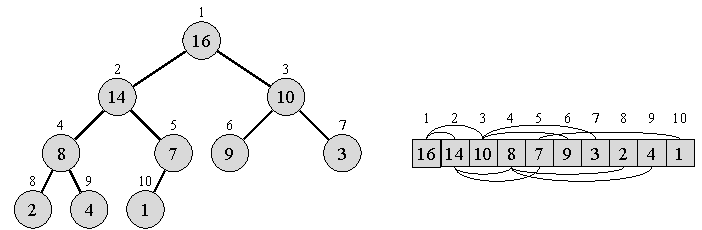
\includegraphics[width=0.9\textwidth]{images/Heap.pdf}
	\caption{A max-heap viewed as an ACB tree (left) and as an array (right)}
\end{figure}

Here we will study min-heap where the value of the children is more than the value of its parent.
\subsection{Initialization}
We create an array $A$ of size $n$. Initially we store the key value of every node to be $\infty$. And for the root $s$ we store $s.\emph{key}=0$.
\subsection{Extracting the Minimum}
For minimum, we already know the root of the heap or the first element of $A$ is the minimum. But after extracting the minimum we need to balance the heap so that it gets the properties of min-heap back. For that we replace the root with the right most element in the array $A$. Then balance the heap by moving it down if one of the child has \emph{key} smaller than \emph{node.key} and keep doing it until both child is larger.
\begin{algorithm}[]
	\caption{\textsc{Extract-Min}$(A)$}
	\SetKwComment{Comment}{// }{}
	\DontPrintSemicolon
	$t\longleftarrow A.\emph{size}$\;
	$Minval\longleftarrow A[1].\emph{key}$\;
	$A[1]\longleftarrow A[t]$\;
	$t\longleftarrow t-1$, $i\longleftarrow 1$\;
	\While{True}{
		\If{$2i\leq t$}{
			$left-val\longleftarrow A[2i].\emph{key}$\;
		}
		\Else{
			\Return{$minval$}\Comment*{No left child i.e. already at leaf}
		}
		\If{$2i+1\leq t$}{
			$right-val\longleftarrow A[2i+1].\emph{key}$
		}
		\Else{
			$right-val\longleftarrow \infty$\Comment*{No right child}
		}
		\If{$left-val\leq right-val$ and $A[i].\emph{key}<left-val$}{
			$curr\_elm\longleftarrow A[i]$\;
			$A[i]\longleftarrow A[2i]$\;
			$U[2i]\longleftarrow curr\_elm$\;
			$i\longleftarrow 2i$
		}
		\ElseIf{$right-val<left-val$}{
			$curr\_elm\longleftarrow A[i]$\;
			$A[i]\longleftarrow A[2i+1]$\;
			$U[2i+1]\longleftarrow curr\_elm$\;
			$i\longleftarrow 2i+1$
		}
		\Else{
			Break
		}
		\Return{$minval$}
	}
\end{algorithm}

In this algorithm for extracting min each time the height of the new root node increases by one at each iteration of the while loop. Hence, this takes at most $O(\log n)$ time.
\subsection{Decreasing Key of a Node}
After decreasing the \emph{key} of a node it may have smaller key than it's parent node. So move it upward i.e. replace with its parent node, and we keep doing it until the parent node has smaller value than it.
\begin{algorithm}[]
	\caption{\textsc{Decrease-Key}$(A,i,k)$}
	\DontPrintSemicolon
	$t\longleftarrow A.\emph{size}$\;
	$A[i]\longleftarrow k$\;
	\While{$i>1$ and $A[i].\emph{key}<A\lt[\lfloor\frac{i}{2}\rfloor\rt].\emph{key}$}{
		$curr\_elm\longleftarrow A[i]$\;
		$A[i].\emph{key}\longleftarrow A\lt[\lfloor\frac{i}{2}\rfloor\rt]$\;
		$A\lt[\lfloor\frac{i}{2}\rfloor\rt]\longleftarrow curr\_elm$\;
		$i\longleftarrow\lt\lfloor\frac{i}{2}\rt\rfloor$
	}
\end{algorithm}
Here again at each iteration of the while loop the height decreases by $1$. Hence, this takes at most $O(\log n)$ time.
\subsection{Time Complexity Analysis of Dijkstra}
Both \textsc{Extract-Min} and \textsc{Decrease-Key} takes $O(\log n)$ time for a min-heap. Now in a Dijkstra algorithm there are $n$ calls for \textsc{Extract-Min} and $m$ calls for \textsc{Decrease-Key}. Therefore, the total time taken by Dijkstra is $O(n\log n)+O(m\log n)=O(m\log n)$. But this is better when $m=o\lt(\frac{n^2}{\log n}\rt)$. Now we will show an improvement of min-heap where the amortized cost of \textsc{Extract-Min} is $O(\log n)$ and amortized cost of \textsc{Decrease-Key} is constant. But first we will take a detour of explaining amortized analysis.
\section{Amortized Analysis}
In amortized analysis, we average the time required to perform a sequence of data-structure operations over all the operations performed. With amortized analysis, we can show that the average cost of an operation is small, if we average over a sequence of operations, even though a single operation within the sequence might be expensive.
\nt{Amortized analysis in not average-case analysis as  amortized analysis guarantees the average performance of each operation in the worst case}

Consider the following algorithm:
\begin{algorithm}[]
	\caption{Amortized Analysis}
	\DontPrintSemicolon
	\KwIn{$n$}
	\Begin{
		$t\longleftarrow 0$, $X(0)\longleftarrow 0^n$\;
		\While{True}{
			$t\longleftarrow t+1$\;
			$X(t)\longleftarrow X(t-1)+1$
		}
	}
\end{algorithm}
Now the number of bit flips in this process is $1,2,1,3,\dots, n,\dots$. At any point the number of bit flips can be at most $n$. In the worst case an operation has cost $n$. We want to compute the average cost for an operation. We will show that starting from $X(0)=0^n$ the average cost is at most $2$. Furthermore, we will show 3 different proofs of this.
\begin{lemma}{}{}
	The total  cost of bit flips for $t$ operations is at most $2t$.
\end{lemma}
\begin{proofmany}{1 (Counting)}
	In $t$ operations:
	\begin{center}
		\begin{tabular}{rl}
			$n^{th}$ bit gets flipped:     & $t$ times                                                    \\
			$(n-1)^{th}$ bit gets flipped: & $\lfloor\frac{t}2\rfloor$ times (when $n^{th}$ bit is 1)     \\
			$(n-2)^{th}$ bit gets flipped: & $\lfloor\frac{t}4\rfloor$ times (when $(n-1)^{th}$ bit is 1) \\
			$\vdots$\hspace{1cm}           & \hspace{1cm}$\vdots$
		\end{tabular}
	\end{center}
	Therefore the total number of bit flips we get is $\leq t\lt(1+\frac12+\frac14+\cdots\rt)\leq 2t$.
\end{proofmany}

Now we will give a proof using the accounting method. In the accounting method of amortized analysis, we assign each operation an amortized cost that may differ from its actual cost. If the amortized cost is higher, the excess is stored as credit on data structure objects; if lower, credit is used to cover the gap. This way, expensive operations can be balanced by cheaper ones, and different operations may have different amortized costs.

\begin{proofmany}{2 (Charging)}
	Suppose every operation costs $2$ Rs. \begin{itemize}
		\item Every change from $0\to 1$ charges $1$ Rs and store $1$ Rs.
		\item Every change from $1\to 0$ charges $2$ Rs.
	\end{itemize}
	Now as you can see to change from $1\to 0$ that bit was previously changed from $0\to 1$. So to change from $1\to 0$ we can use the stored $1$ Rs. Hence, in average every operation costs exactly $0$ to $1$ Rs. Since there are $t$ operations total number of bit flips is at most $2t$.
\end{proofmany}

In the next proof we will analyze by computing a necessary potential function. After each operation we can calculate the potential difference.

\begin{proofmany}{3 (Potential)}
	Consider the potential function $\Phi(i)=\#$1's in $X(i)$. Let at $i^{th}$ operation $t_i$ bits were flipped from $1\to 0$. Now any operation flips at most $1$ bit from $0\to 1$. Therefore, number of bit flips in $i^{th}$ operation is at most $t_i+1$. Therefore, we have $$\Phi(i)\leq \Phi(i-1)-t_i+1$$since the number of $1$'s in $\Phi(i)$ is decreased by $t_i$ many $1\to 0$ flips and then $1$ flip from $0\to 1$. Therefore, the cost at $i^{th}$ operation is at most $\Phi(i-1)-\Phi(i)+2$. Hence, the total number of bit flips in $t$ operations is $\Phi(0)-\Phi(t)+2t\leq 2t$.
\end{proofmany}

Hence, after $t$ operations the total number of bit flips is at most $2t$. Therefore, on average the cost per operation is at most $2$. Hence, the amortized cost of the operation is $2$. So we will use such amortized analysis on the next data structure to optimize the run time of Dijkstra Algorithm.
\section{Data Structure 3: Fibonacci Heap}
Instead of keeping just one Heap we will now keep an array of Heaps. We will also discard the idea of binary trees. We will now use a data structure which will take the benefit of the faster time of both the data structure. I.e.
\begin{center}
	\begin{tabular}{c|c|c}
		               & \prb{Extract-Min}                                       & \prb{Decrease-Key}                                 \\
		Linear Array   & $O(n)$                                                  & $\mathcolor{red}{\boxed{\mathcolor{black}{O(1)}}}$ \\
		Min-Heap       & $\mathcolor{red}{\boxed{\mathcolor{black}{O(\log n)}}}$ & $O(\log n)$                                        \\[2mm]
		Fibonacci Heap & $O(\log n)^*$                                           & $O(1)^*$
	\end{tabular}
\end{center}
The * is because  in Fibonacci Heap the amortized time taken by \prb{Extract-Min} is  $O(\log n)$.

Since Fibonacci heap is an array of heaps there is a \emph{rootlist} which is the list of all the roots of all the heaps in the Fibonacci heap. There is a \emph{min-pointer} which points to the root with the minimum key. For each node in the Fibonacci heap we have a pointer to its parent and  we keep 3 variables. The 3 variables are \emph{degree}, \emph{size} and \emph{lost} where \emph{lost} is a Boolean Variable. \begin{itemize}
	\item For any node $x$ in the Fibonacci heap the $x.\emph{degree}$ is the number of children $x$ has.
	\item $x.\emph{size}$ is the number of nodes in the tree rooted at $x$.
	\item $x.\emph{lost}$ is 1 if and only if $x$ has lost a child before.
\end{itemize} Why any node will lose a child that explanation we will give later. With this set up let's dive into the data structure.

\begin{figure}[h!]
	\centering
	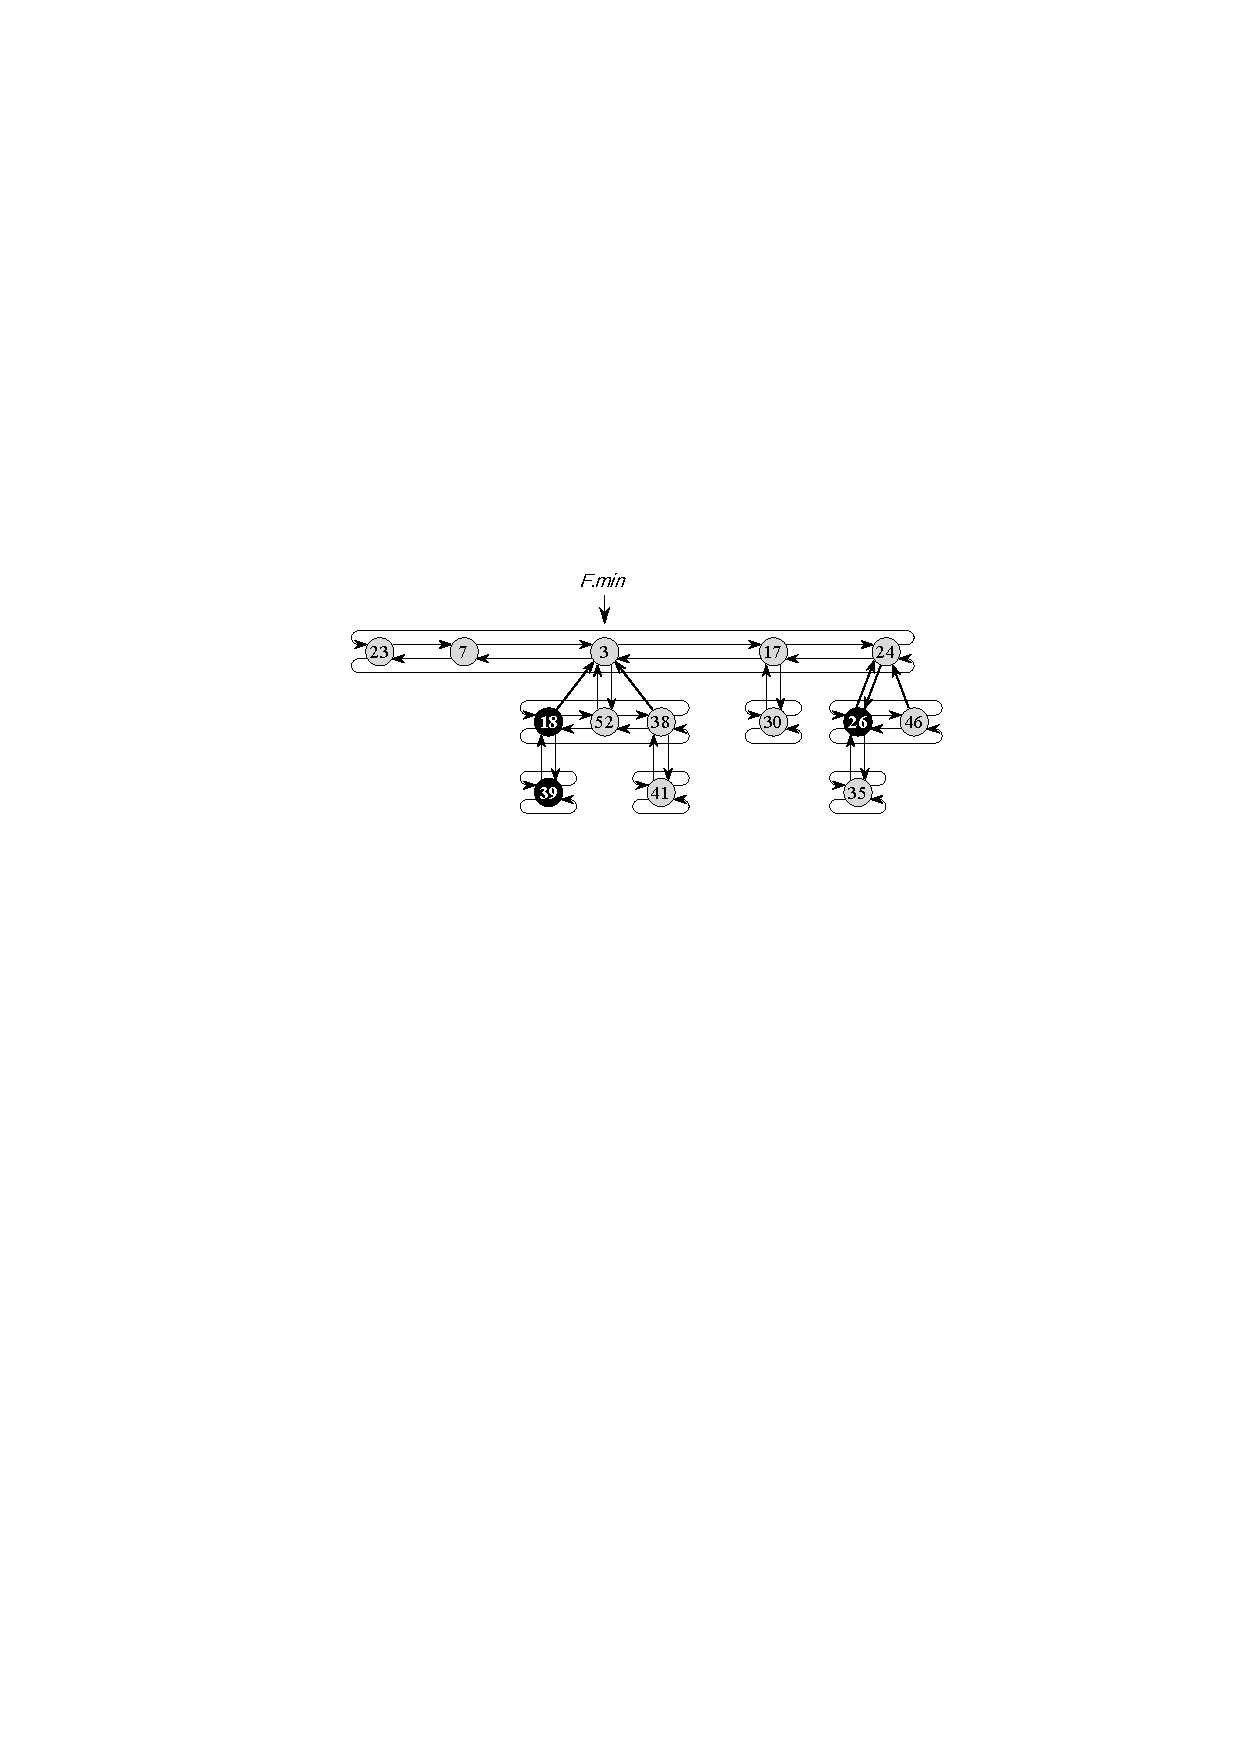
\includegraphics{images/Fibheap1.pdf}
	\caption{A Fibonacci Heap with 5 heaps in the rootlist}
\end{figure}
\subsection{Inserting Node}
To insert a node we call the \prb{Fib-Insert} function and in the function the algorithm initiates the node with setting up all the pointers and variables then add the node to the \emph{rootlist}.\parinf

\begin{minipage}{0.45\textwidth}
	\begin{algorithm}[H]
		\DontPrintSemicolon
		\caption{\textsc{Fib-Create-Node}$(v)$}
		$x.\emph{degree}\longleftarrow 0$\;
		$x.\emph{parent}\longleftarrow None$\;
		$x.\emph{child}\longleftarrow None$\;
		$x.\emph{lost}\longleftarrow 0$\;
		$x.\emph{key}\longleftarrow v$\;
		\Return{$x$}
	\end{algorithm}
\end{minipage}\hfill
\begin{minipage}{0.45\textwidth}
	\begin{algorithm}[H]
		\DontPrintSemicolon
		\caption{\textsc{Fib-Insert}$(F,v)$}
		$x\longleftarrow \textsc{Create-Node}(v)$\;
		\If{$F.\min==None$}{
			$F.\emph{rootlist}\longleftarrow [x]$\;
			$F.\min\longleftarrow x$\;
		}
		\Else{
			$F.\emph{rootlist}.\emph{append}(x)$\;
			\If{$x.key<F.\min.key$}{
				$F.min\longleftarrow x$
			}
		}
	\end{algorithm}
\end{minipage}

All of this can be done in $O(1)$ time. Therefore, to insert a node in the Fibonacci heap it takes $O(1)$ time.
\subsection{Union of Fibonacci Heaps}
To unite to Fibonacci heaps $F_1$ and $F_2$ we simply concatenate the root lists of $F_1$ and $F_2$ and then determine the new minimum node.
\begin{algorithm}
	\DontPrintSemicolon
	\caption{\textsc{Fib-Union}$(F_1,F_2)$}
	$F\longleftarrow \textsc{Make-Fib-Heap}$\;
	$F.\min\longleftarrow F_1.\min$\;
	$F.\emph{rootlist}\longleftarrow F_1.\emph{rootlist} ++ F_2.\emph{rootlist}$\;
	\If{$F_2.\min<F_1.\min$}{
		$F.\min\longleftarrow F_2.\min$
	}
	\Return{$F$}
\end{algorithm}
All the operations here can be done in constant time. Hence, \textsc{Fib-Union} takes $O(1)$ time.
\subsection{Extracting the Minimum Node}
The \textsc{Fib-Extract-Min} function extracts the minimum node from the Fibonacci heap $F$ and then rearranges the heap array. It works by first making a root node out of each of the minimum node's children and removing the minimum node from the rootlist. It then consolidates the root list by linking roots of equal degree until at most one root remains of each degree.
\begin{center}
	\begin{minipage}{0.45\textwidth}
		\begin{algorithm}[H]
			\caption{\textsc{Fib-Extract-Min}$(F)$}
			\DontPrintSemicolon
			$z\longleftarrow F.\min$\;
			\If{$z\neq None$}{
				\For{$x\in z.\emph{child}$}{
					$F.\emph{rootlist}.\emph{append}(x)$\;
					$x.\emph{parent}\longleftarrow None$
				}
				Remove $z$ from $F.\emph{rootlist}$\;
				\If{$z==z.\emph{right}$}{
					$F.\min\longleftarrow None$\;
				}
				\Else{
					$F.\min\longleftarrow z.\emph{right}$
					\emph{consolidate}($F$)
				}
			}
			\Return{$z$}
		\end{algorithm}
		\vspace{2.8cm}

		\begin{algorithm}[H]
			\caption{\textsc{Fib-Heap-Link}$(H,y,x)$}
			\DontPrintSemicolon
			Remove $y$ from $F.\emph{rootlist}$\;
			$y.\emph{parent}\longleftarrow x$\;
			$y.\emph{lost}\longleftarrow 0$
		\end{algorithm}
	\end{minipage}\hfill
	\begin{minipage}{0.5\textwidth}
		\begin{algorithm}[H]
			\caption{\textsc{Consolidate}$(F)$}
			\DontPrintSemicolon
			Initialize array $A[0,\dots, D(n)]$ with \emph{None} elements.\;
			\For{$x\in F.\emph{rootlist}$}{
				$d\longleftarrow x.\emph{degree}$\;
				\If{$A[d]==None$}{
					$A[d]\longleftarrow x$
				}
				\While{$A[d]\neq None$}{
					$y\longleftarrow A[d]$\;
					\If{$y.\emph{key}<x.\emph{key}$}{
						Exchange $x$ with $y$
					}
					\emph{Fib-Heap-Link}$(F,y,x)$\;
					$A[d]\longleftarrow None$, $d\longleftarrow d+1$\;
				}
				$A[d]\longleftarrow x$
			}
			$F.\min\longleftarrow None$\;
			\For{$i=0$ to $D$}{
				\If{$A[i]\neq None$}{
					\If{$F.\min==None$}{
						$F.\emph{rootlist}\longleftarrow [A[i]]$, $F.\min\longleftarrow A[i]$\;
					}
					\Else{
						$F.\emph{rootlist}.\emph{append}(A[i])$\;
						\If{$A[i].\emph{key}<F.\min.\emph{key}$}{
							$F.\min\longleftarrow A[i]$
						}
					}
				}
			}
		\end{algorithm}
	\end{minipage}
\end{center}

Here $D(n)$ denotes the maximum degree a node can have after \textsc{Consolidate}. The procedure \textsc{Consolidate} uses an auxiliary array of size $A$ of size $D$ which we will choose later. For each $i\leq D(n)$ it keeps a heap of degree $i$. And if it finds two 
\begin{figure}[h!]
	\centering
	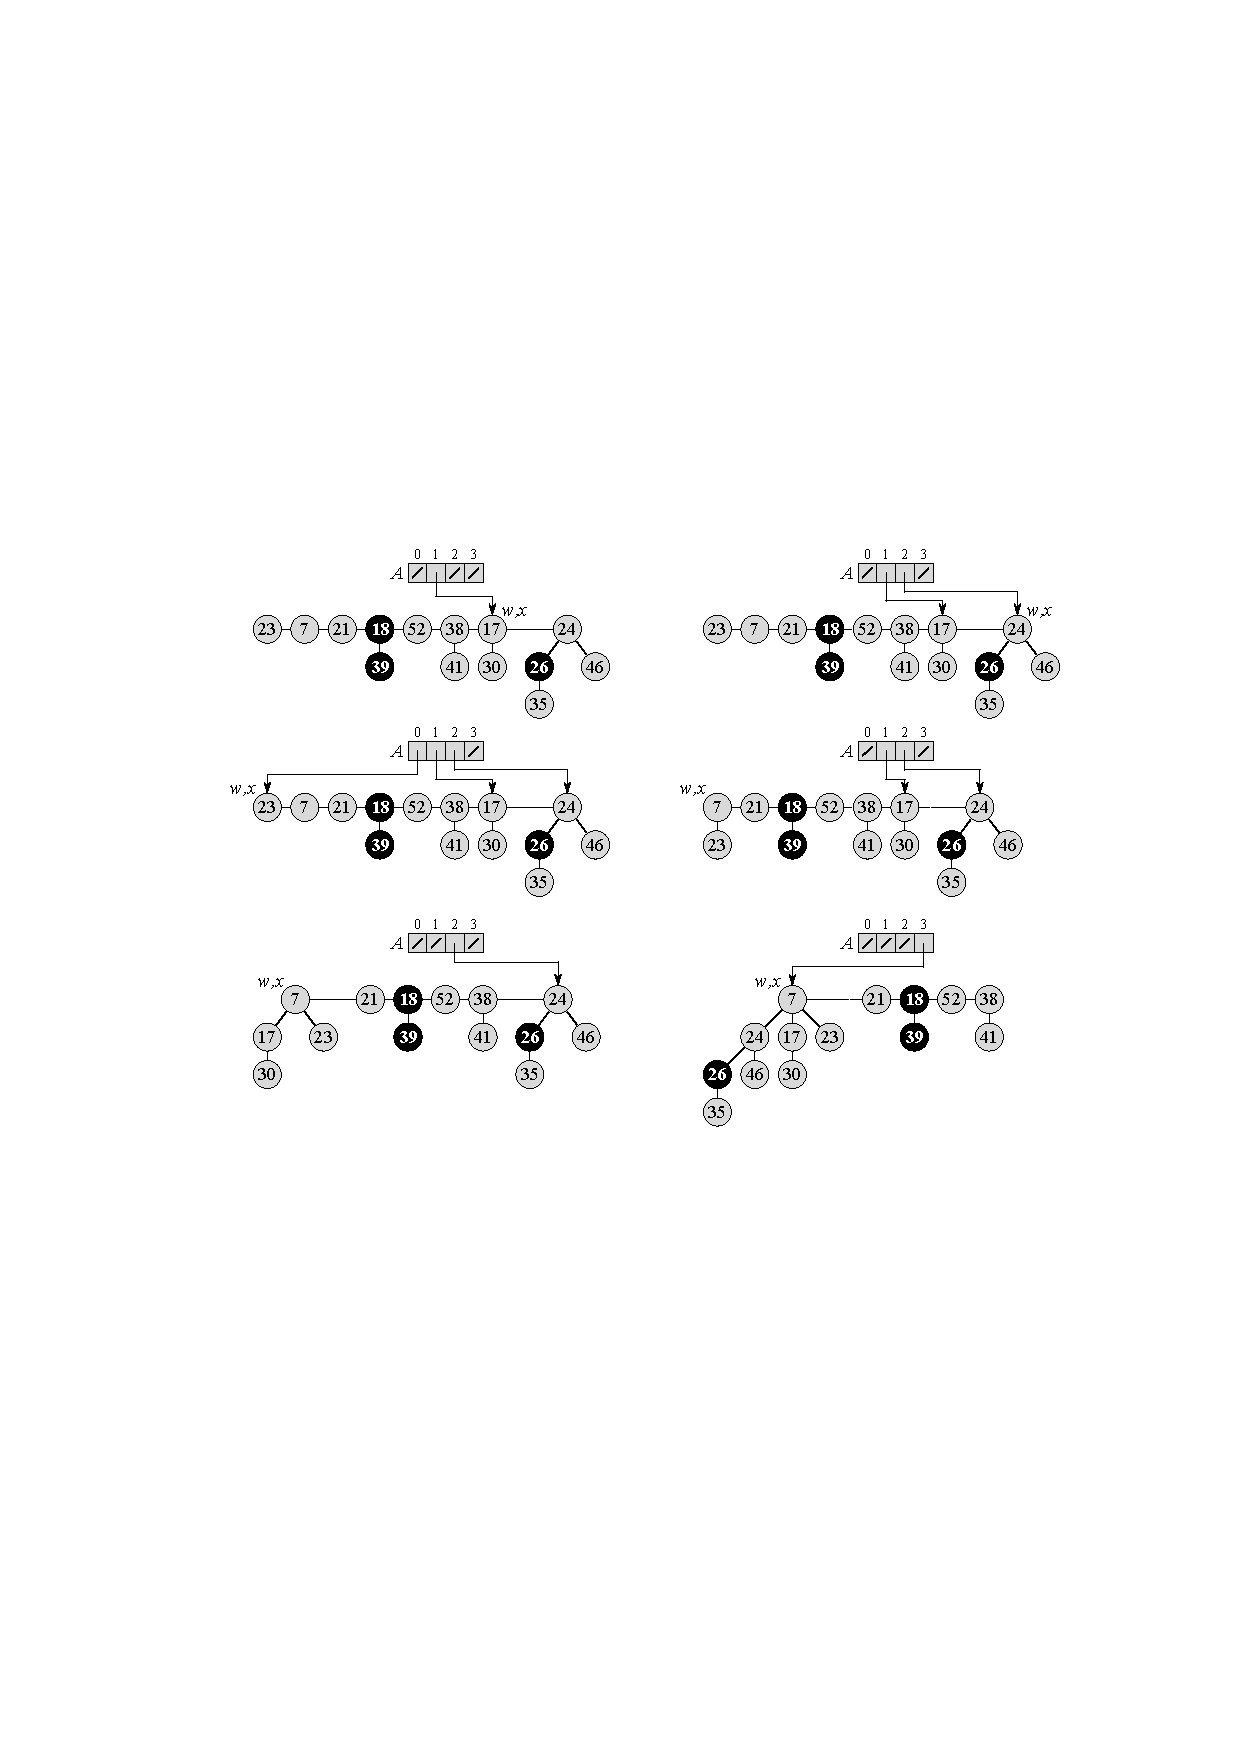
\includegraphics[width=0.75\textwidth]{images/Fibheap2.pdf}
	\caption{A run of \textsc{Consolidate}}
\end{figure}
heaps of same degree then it makes the one with higher key to be the child of the other one. The function \textsc{Fib-Heap-Link} does this process of linking two heaps of same degree.\parinn

Of course in order to allocate array we have to know how to calculate the upper bound for $D(n)$ on the maximum degree. We will show an upper bound of $O(\log n)$ in \autoref{max-degree-bound}.

Now in \textsc{Fib-Extract-Min} in each iteration of the outer for loop or inner while loop it operates on one heap in $F.\emph{rootlist}$. Hence it takes $O(D(n)+\#\text{heaps in $F.\emph{rootlist}$})$ time.


\subsection{Decreasing Key of a Node}
In this section we will show how to decrease a key of a node in a Fibonacci heap in $O(1)$ amortized time. The \textsc{Fib-Decrease-Key} function decreases the key value of the target node then if the min-heap order the node is in is violated then we use the \textsc{Cascading-Cut} function to restore the min-heap property again. These two functions operates like the following:
\begin{center}
	\begin{minipage}{0.45\textwidth}
		\begin{algorithm}[H]
			\caption{\textsc{Fib-Decrease-Key}$(F,x,k)$}
			\DontPrintSemicolon
			\If{$k>x.\emph{key}$}{
				\Return{Error}
			}
			$x.\emph{key}\longleftarrow k$\;
			$y\longleftarrow x.\emph{parent}$\;
			\If{$y\neq None$ and $x.\emph{key}<y.\emph{key}$}{
				\textsc{Cut}$(F,x,y)$\;
				\textsc{Cascading-Cut}$(F,y)$\;
			}
			\If{$k<F.\min.\emph{key}$}{
				$F.\min\longleftarrow x$
			}
		\end{algorithm}
	\end{minipage}\hfill
	\begin{minipage}{0.45\textwidth}
		\begin{algorithm}[H]
			\caption{\textsc{Cascading-Cut}$(F,y)$}
			\DontPrintSemicolon
			% $z\longleftarrow y.\emph{parent}$\;
			\If{$y.\emph{parent}\neq None$}{
				\If{$y.\emph{lost}==0$}{
					$y.\emph{lost}\longleftarrow 1$\;
				}
				\Else{
					\textsc{Cut}$(F,y,y.\emph{parent})$\;
					\textsc{Cascading-Cut}$(F,y.\emph{parent})$
				}
			}
		\end{algorithm}
		\begin{algorithm}[H]
			\caption{\textsc{Cut}$(F,x,y)$}
			\DontPrintSemicolon
			Remove $x$ from $y.\emph{child}$\;
			$y.\emph{degree}\longleftarrow y.\emph{degree}-1$\;
			$F.\emph{rootlist}.\emph{append}(x)$\;
			$x.\emph{parent}\longleftarrow None$, $x.\emph{lost}\longleftarrow 0$\;
		\end{algorithm}
	\end{minipage}
\end{center}
After decreasing the key of the target node if the min-heap order has been violated then we start by cutting the link between $x$ and its parent by adding it to the rootlist. Let $x$ is a node in $F$. At some time $x$ was a root. 
\begin{figure}[h!]
	\centering
	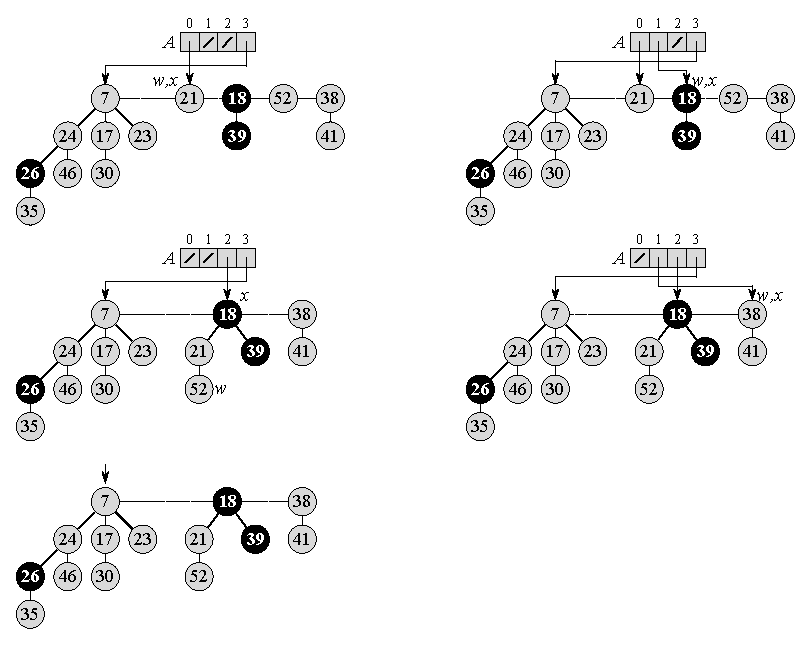
\includegraphics[width=0.7\textwidth]{images/Fibheap3.pdf}
	\caption{A run of \textsc{Cascading-Cut}}
\end{figure}Then $x$ was linked to another node. Suppose at some time two children of $x$ were removed by cuts. As soon as second child has been lost we cut $x$ from its parent and make it a new root. But we are not done yet. Since $x$ might be the second child cut from its parent. So we have to check for its parent. Therefore, we recursively run \textsc{Cascading-Cut} on its parent till we reach the root or cut the first child from a node.

Notice at each run of \textsc{Cascading-Cut} the \emph{lost} bit of a node is getting reset. Therefore, the total time taken by \textsc{Fib-Decrease-Key} is $O(1+\#\text{lost bits reset})$.
\subsection{Bounding the Maximum Degree}\label{max-degree-bound}
To prove that the amortized time of \textsc{Fib-Extract-Min} and \textsc{Fib-Delete} is $O(\log n)$ we must show that upper bound of the maximum degree of any node after \textsc{Consolidate} function is $O(\log n)$. In particular, we will show its $\lt\lfloor \log_{\phi}n\rt\rfloor$ where $\phi$ is the golden ratio.
\begin{lemma}{}{}
	Let $x$ be any node in a Fibonacci heap, and suppose that $x.\emph{degree}=k$. Let $y_1,\dots, y_k$ denote the children of $x$ in the order in which they were linked to $x$ from the earliest to the latest. Then $y_1.\emph{degree}\geq 0$ and $y_i.\emph{degree}\geq i-2$ for $i=2,\dots, k$.
\end{lemma}
\begin{proof}
	Obviously $y_1.\emph{degree}\geq 0$. The only function that adds a child to a node is the function \textsc{Consolidate}. Now for $i\geq 2$, $y_i$ was linked to $x$ when all of $y_1,\dots, y_{i-1}$ were children of $x$, and therefore we must have had $x.\emph{degree}\geq i-1$. Because node $y_i$ is linked to $x$ only if $x\emph{degree}=y_i.\emph{degree}$ we must also have $y_i.\emph{degree}\geq i-1$. Since then node $y_i$ has lost at most one child, since it would have been cut from $x$ by \textsc{Cascading-Cut} if it had lost two children. We conclude that $y_i.\emph{degree}\geq i-2$.
\end{proof}
\begin{lemma}{}{}
	Let $x$ be a node in a Fibonacci heap and let $k=x.\emph{degree}$. Then $$\emph{size}(x)\geq F_{k+2}\geq \phi^k$$
\end{lemma}
\begin{proof}
	We will prove this using induction. For $k=0$, $F_2=1$ so this is obviously true. For $k=1$ there is one child of $x$. Hence, $\emph{size}(x)=2=F_3$. Suppose this is true for $1,\dots, k-1$. Let $y_1,\dots, y_k$ are the children of $x$  in the order in which they were linked to $x$. By the above lemma we have $y_1.\emph{degree}\geq 0$ and $y_i.\emph{degree}\geq i-2$ for all $i=2,\dots, k$. Hence, by Induction hypothesis we have $\emph{size}(y_i)\geq F_{i-2}$ for all $i=2,\dots, k$. Therefore, \[
		\emph{size}(x) \geq 1+\sum\limits_{i=1}^{k}\emph{size}(y_k)\geq 2+\sum\limits_{i=2}^kF_{k}=1+\sum\limits_{i=0}^k F_k=F_{k+2}\geq \phi^k
	\]Hence, we have the lemma.
\end{proof}
\begin{corollary}{}{}
	The maximum degree of any node in \textsc{Consolidate}, $D(n)=O(\log n)$.
\end{corollary}
\subsection{Time Complexity Analysis of Dijkstra}

Now we will calculate the amortized time of Dijkstra algorithm. Before that we will calculate the amortized cost of the data structure. Let in an algorithm  \textsc{Fib-Extract-Min} was called $t$ times. Therefore, total cost of all $t$ many \textsc{Fib-Extract-Min} calls is $O(t\log n+\text{total $\#$heaps created})$. Now heaps are created because of \textsc{Fib-Extract-Min} functions and \textsc{Fib-Decrease-Key} function. We know \textsc{Fib-Extract-Min} were called $t$ times and each time it created $O(\log n)$ heaps. Hence, in total \textsc{Fib-Extract-Min} created $O(t\log n)$ heaps. Therefore, time taken by the $t$ many \textsc{Fib-Extract-Min} calls is $O(t\log n+\#\textsc{Fib-Decrease-Key}\text{ calls})$.

Now suppose in an algorithm $k$ times the function \textsc{Fib-Decrease-Key} function were called. Hence, this takes $O(k+\#\text{total number of \textsc{lost} bits reset})=O(k+\#\text{total number of \textsc{lost} bits rset})$ time. Now the \emph{lost} bits are set only by the \textsc{Fib-Decrease--Key}. Therefore, $\#\text{total number of \textsc{lost} bits rset}=\#\text{\textsc{Fib-Decrese-Key} was called}$. Therefore, the total time taken by all the \textsc{Fib-Decrese-Key} calls is $O(k)$.

Hence, in an algorithm if $t$ times \textsc{Fib-Extract-Min} was called and $k$ times \textsc{Fib-Decrese-Key} was called then total time taken by \textsc{Fib-Extract-Min} is $O(t\log n+k)$ and total time taken by \textsc{Fib-Decrese-Key} is $O(k)$. Therefore, amortized time taken by \textsc{Fib-Extract-Min} is $O(\frac{t}{k}\log n)$ and by \textsc{Fib-Decrese-Key} is $O(1)$.

Now in the Dijkstra algorithm \textsc{Fib-Extract-Min} is called $n$ times and \textsc{Fib-Decrese-Key} is called $O(m)$ times where $n$ is the number of vertices in the graph and $m$ is the number of edges in the graph. Hence, the amortized cost of \textsc{Fib-Extract-Min} is $O(\log n)$ and \textsc{Fib-Decrease-Key} is $O(1)$. Therefore, using Fibonacci heap Dijkstra takes $(n\log n+m)$ time.

\chapter{Kruskal Algorithm with Data Structure}

\section{Kruskal Algorithm}
\begin{center}
\hspace*{4mm}\begin{tikzpicture}[vertex/.style={circle, draw, fill=white, inner sep=2pt}]
\begin{scope}[shift={(-5,0)}]
		\node[vertex] (1) at (0, 0) {};
	\node[vertex] (2) at (1, 1) {};
	\node[vertex] (3) at (1, -1) {};
	\node[vertex] (4) at (2, 0) {};
	\node[vertex] (5) at (4, 0.5) {};
	\node[vertex] (6) at (6, 2) {};
	\node[vertex] (7) at (5, -0.5) {};
	\node[vertex] (8) at (3, -1) {};
	\node[vertex] (9) at (0, -2) {};
	
	%    % Edges with weights (some edges have bends to avoid crossing)
	\draw[shorten >=1pt, shorten <=1pt] (1) -- (2) node[midway, xshift=-1mm,yshift=2mm] {6};
	\draw[shorten >=1pt, shorten <=1pt] (1) -- (3) node[midway, xshift=1mm,yshift=2mm] {3};
	\draw[shorten >=1pt, shorten <=1pt] (2) -- (3) node[midway, right] {14};
	\draw[shorten >=1pt, shorten <=1pt] (2) -- (4) node[midway, above right] {12};
	\draw[shorten >=1pt, shorten <=1pt] (3) -- (4) node[midway, xshift=1mm,yshift=-2mm] {2};
	\draw[shorten >=1pt, shorten <=1pt] (4) -- (5) node[midway, below right] {7};
	\draw[shorten >=1pt, shorten <=1pt] (2) to [bend left=60] (5) node[xshift=-1.5cm, yshift=1.2cm] {15};
	\draw[shorten >=1pt, shorten <=1pt] (5) -- (6) node[midway, above left] {18};
	\draw[shorten >=1pt, shorten <=1pt] (6) -- (7) node[midway, xshift=-3mm, yshift=-1mm] {24};
	\draw[shorten >=1pt, shorten <=1pt] (7) -- (8) node[midway, above left]{16};
	\draw[shorten >=1pt, shorten <=1pt] (3) -- (8) node[midway, below] {5};
	\draw[shorten >=1pt, shorten <=1pt] (3) to [bend right=80, looseness=1.5] (6) node[xshift=-1.5cm, yshift=-4.1cm] {10};
	\draw[shorten >=1pt, shorten <=1pt] (3) -- (9) node[midway, xshift=-1mm,yshift=2mm] {9};
\end{scope}
\draw[ultra thick, -Stealth] (2,0)  -- (4.2,0) node[midway, above] {Kruskal} node[midway, below] {Algorithm};
\begin{scope}[shift={(5,0)}]
	\node[vertex] (1) at (0, 0) {};
	\node[vertex] (2) at (1, 1) {};
	\node[vertex] (3) at (1, -1) {};
	\node[vertex] (4) at (2, 0) {};
	\node[vertex] (5) at (4, 0.5) {};
	\node[vertex] (6) at (6, 2) {};
	\node[vertex] (7) at (5, -0.5) {};
	\node[vertex] (8) at (3, -1) {};
	\node[vertex] (9) at (0, -2) {};
	
	%    % Edges with weights (some edges have bends to avoid crossing)
	\draw[shorten >=1pt, shorten <=1pt, red, thick] (1) -- (2) node[midway, xshift=-1mm,yshift=2mm] {6};
	\draw[shorten >=1pt, shorten <=1pt, red, thick] (1) -- (3) node[midway, xshift=1mm,yshift=2mm] {3};
	\draw[shorten >=1pt, shorten <=1pt] (2) -- (3) node[midway, right] {14};
	\draw[shorten >=1pt, shorten <=1pt] (2) -- (4) node[midway, above right] {12};
	\draw[shorten >=1pt, shorten <=1pt, red, thick] (3) -- (4) node[midway, xshift=1mm,yshift=-2mm] {2};
	\draw[shorten >=1pt, shorten <=1pt, red, thick] (4) -- (5) node[midway, below right] {7};
	\draw[shorten >=1pt, shorten <=1pt] (2) to [bend left=60] (5) node[xshift=-1.5cm, yshift=1.2cm] {15};
	\draw[shorten >=1pt, shorten <=1pt] (5) -- (6) node[midway, above left] {18};
	\draw[shorten >=1pt, shorten <=1pt] (6) -- (7) node[midway, xshift=-3mm, yshift=-1mm] {24};
	\draw[shorten >=1pt, shorten <=1pt, red, thick] (7) -- (8) node[midway, above left]{16};
	\draw[shorten >=1pt, shorten <=1pt, red, thick] (3) -- (8) node[midway, below] {5};
	\draw[shorten >=1pt, shorten <=1pt, red, thick] (3) to [bend right=80, looseness=1.5] (6) node[xshift=-1.5cm, yshift=-4.1cm] {10};
	\draw[shorten >=1pt, shorten <=1pt, red, thick] (3) -- (9) node[midway, xshift=-1mm,yshift=2mm] {9};
\end{scope}
\end{tikzpicture}
\end{center}

\section{Data Structure 1: Array}

\section{Data Structure 2: Left Child Right Siblings Tree}

\section{Data Structure 3: Union Find}
\end{document}
